\documentclass[twoside]{book}

% Packages required by doxygen
\usepackage{fixltx2e}
\usepackage{calc}
\usepackage{doxygen}
\usepackage{graphicx}
\usepackage[utf8]{inputenc}
\usepackage{makeidx}
\usepackage{multicol}
\usepackage{multirow}
\PassOptionsToPackage{warn}{textcomp}
\usepackage{textcomp}
\usepackage[nointegrals]{wasysym}
\usepackage[table]{xcolor}

% Font selection
\usepackage[T1]{fontenc}
\usepackage{mathptmx}
\usepackage[scaled=.90]{helvet}
\usepackage{courier}
\usepackage{amssymb}
\usepackage{sectsty}
\renewcommand{\familydefault}{\sfdefault}
\allsectionsfont{%
  \fontseries{bc}\selectfont%
  \color{darkgray}%
}
\renewcommand{\DoxyLabelFont}{%
  \fontseries{bc}\selectfont%
  \color{darkgray}%
}
\newcommand{\+}{\discretionary{\mbox{\scriptsize$\hookleftarrow$}}{}{}}

% Page & text layout
\usepackage{geometry}
\geometry{%
  a4paper,%
  top=2.5cm,%
  bottom=2.5cm,%
  left=2.5cm,%
  right=2.5cm%
}
\tolerance=750
\hfuzz=15pt
\hbadness=750
\setlength{\emergencystretch}{15pt}
\setlength{\parindent}{0cm}
\setlength{\parskip}{0.2cm}
\makeatletter
\renewcommand{\paragraph}{%
  \@startsection{paragraph}{4}{0ex}{-1.0ex}{1.0ex}{%
    \normalfont\normalsize\bfseries\SS@parafont%
  }%
}
\renewcommand{\subparagraph}{%
  \@startsection{subparagraph}{5}{0ex}{-1.0ex}{1.0ex}{%
    \normalfont\normalsize\bfseries\SS@subparafont%
  }%
}
\makeatother

% Headers & footers
\usepackage{fancyhdr}
\pagestyle{fancyplain}
\fancyhead[LE]{\fancyplain{}{\bfseries\thepage}}
\fancyhead[CE]{\fancyplain{}{}}
\fancyhead[RE]{\fancyplain{}{\bfseries\leftmark}}
\fancyhead[LO]{\fancyplain{}{\bfseries\rightmark}}
\fancyhead[CO]{\fancyplain{}{}}
\fancyhead[RO]{\fancyplain{}{\bfseries\thepage}}
\fancyfoot[LE]{\fancyplain{}{}}
\fancyfoot[CE]{\fancyplain{}{}}
\fancyfoot[RE]{\fancyplain{}{\bfseries\scriptsize Generated on Mon Dec 1 2014 11\+:46\+:48 for My Project by Doxygen }}
\fancyfoot[LO]{\fancyplain{}{\bfseries\scriptsize Generated on Mon Dec 1 2014 11\+:46\+:48 for My Project by Doxygen }}
\fancyfoot[CO]{\fancyplain{}{}}
\fancyfoot[RO]{\fancyplain{}{}}
\renewcommand{\footrulewidth}{0.4pt}
\renewcommand{\chaptermark}[1]{%
  \markboth{#1}{}%
}
\renewcommand{\sectionmark}[1]{%
  \markright{\thesection\ #1}%
}

% Indices & bibliography
\usepackage{natbib}
\usepackage[titles]{tocloft}
\setcounter{tocdepth}{3}
\setcounter{secnumdepth}{5}
\makeindex

% Hyperlinks (required, but should be loaded last)
\usepackage{ifpdf}
\ifpdf
  \usepackage[pdftex,pagebackref=true]{hyperref}
\else
  \usepackage[ps2pdf,pagebackref=true]{hyperref}
\fi
\hypersetup{%
  colorlinks=true,%
  linkcolor=blue,%
  citecolor=blue,%
  unicode%
}

% Custom commands
\newcommand{\clearemptydoublepage}{%
  \newpage{\pagestyle{empty}\cleardoublepage}%
}


%===== C O N T E N T S =====

\begin{document}

% Titlepage & ToC
\hypersetup{pageanchor=false,
             bookmarks=true,
             bookmarksnumbered=true,
             pdfencoding=unicode
            }
\pagenumbering{roman}
\begin{titlepage}
\vspace*{7cm}
\begin{center}%
{\Large My Project }\\
\vspace*{1cm}
{\large Generated by Doxygen 1.8.8}\\
\vspace*{0.5cm}
{\small Mon Dec 1 2014 11:46:48}\\
\end{center}
\end{titlepage}
\clearemptydoublepage
\tableofcontents
\clearemptydoublepage
\pagenumbering{arabic}
\hypersetup{pageanchor=true}

%--- Begin generated contents ---
\chapter{Hierarchical Index}
\section{Class Hierarchy}
This inheritance list is sorted roughly, but not completely, alphabetically\+:\begin{DoxyCompactList}
\item \contentsline{section}{\+\_\+\+\_\+character$<$ T, N $>$}{\pageref{class____character}}{}
\item \contentsline{section}{\+\_\+\+\_\+character$<$ char, N $>$}{\pageref{class____character_3_01char_00_01_n_01_4}}{}
\item \contentsline{section}{\+\_\+\+\_\+character$<$ unsigned char, N $>$}{\pageref{class____character_3_01unsigned_01char_00_01_n_01_4}}{}
\item \contentsline{section}{\+\_\+\+\_\+character$<$ wchar\+\_\+t, N $>$}{\pageref{class____character_3_01wchar__t_00_01_n_01_4}}{}
\item \contentsline{section}{backup\+\_\+variable$<$ T $>$}{\pageref{classbackup__variable}}{}
\item binary\+\_\+function\begin{DoxyCompactList}
\item \contentsline{section}{string\+\_\+util\+:\+:equal\+\_\+string\+\_\+i\+\_\+compare$<$ T $>$}{\pageref{classstring__util_1_1equal__string__i__compare}}{}
\item \contentsline{section}{string\+\_\+util\+:\+:less\+\_\+string\+\_\+compare$<$ T $>$}{\pageref{classstring__util_1_1less__string__compare}}{}
\item \contentsline{section}{string\+\_\+util\+:\+:less\+\_\+string\+\_\+i\+\_\+compare$<$ T $>$}{\pageref{classstring__util_1_1less__string__i__compare}}{}
\item \contentsline{section}{string\+\_\+util\+:\+:less\+\_\+string\+\_\+n\+\_\+compare$<$ T $>$}{\pageref{classstring__util_1_1less__string__n__compare}}{}
\item \contentsline{section}{string\+\_\+util\+:\+:less\+\_\+string\+\_\+natural\+\_\+order\+\_\+i\+\_\+compare$<$ T $>$}{\pageref{classstring__util_1_1less__string__natural__order__i__compare}}{}
\item \contentsline{section}{string\+\_\+util\+:\+:less\+\_\+string\+\_\+ni\+\_\+compare$<$ T $>$}{\pageref{classstring__util_1_1less__string__ni__compare}}{}
\end{DoxyCompactList}
\item \contentsline{section}{Document\+Parser}{\pageref{class_document_parser}}{}
\item \contentsline{section}{Index\+Handler}{\pageref{class_index_handler}}{}
\begin{DoxyCompactList}
\item \contentsline{section}{A\+V\+L\+Tree}{\pageref{class_a_v_l_tree}}{}
\item \contentsline{section}{Hash\+Table}{\pageref{class_hash_table}}{}
\end{DoxyCompactList}
\item \contentsline{section}{stemming\+:\+:no\+\_\+op\+\_\+stem$<$ string\+\_\+type\+T $>$}{\pageref{classstemming_1_1no__op__stem}}{}
\item \contentsline{section}{Node}{\pageref{class_node}}{}
\begin{DoxyCompactList}
\item \contentsline{section}{A\+V\+L\+Node}{\pageref{class_a_v_l_node}}{}
\item \contentsline{section}{Hash\+Node}{\pageref{class_hash_node}}{}
\end{DoxyCompactList}
\item \contentsline{section}{Page}{\pageref{class_page}}{}
\item \contentsline{section}{Query}{\pageref{class_query}}{}
\item \contentsline{section}{Query\+Processor}{\pageref{class_query_processor}}{}
\item \contentsline{section}{stemming\+:\+:stem$<$ string\+\_\+type\+T $>$}{\pageref{classstemming_1_1stem}}{}
\begin{DoxyCompactList}
\item \contentsline{section}{stemming\+:\+:english\+\_\+stem$<$ string\+\_\+type\+T $>$}{\pageref{classstemming_1_1english__stem}}{}
\end{DoxyCompactList}
\item \contentsline{section}{Stem\+Helper}{\pageref{class_stem_helper}}{}
\item \contentsline{section}{stemmer}{\pageref{structstemmer}}{}
\item \contentsline{section}{string\+\_\+util\+:\+:string\+\_\+trim$<$ char\+\_\+type\+T $>$}{\pageref{classstring__util_1_1string__trim}}{}
\item unary\+\_\+function\begin{DoxyCompactList}
\item \contentsline{section}{even$<$ T $>$}{\pageref{classeven}}{}
\item \contentsline{section}{within$<$ T $>$}{\pageref{classwithin}}{}
\end{DoxyCompactList}
\item \contentsline{section}{User\+Interface}{\pageref{class_user_interface}}{}
\end{DoxyCompactList}

\chapter{Class Index}
\section{Class List}
Here are the classes, structs, unions and interfaces with brief descriptions\+:\begin{DoxyCompactList}
\item\contentsline{section}{\hyperlink{class_a_v_l_node}{A\+V\+L\+Node} }{\pageref{class_a_v_l_node}}{}
\item\contentsline{section}{\hyperlink{class_a_v_l_tree}{A\+V\+L\+Tree} }{\pageref{class_a_v_l_tree}}{}
\item\contentsline{section}{\hyperlink{class_document_parser}{Document\+Parser} }{\pageref{class_document_parser}}{}
\item\contentsline{section}{\hyperlink{class_hash_node}{Hash\+Node} }{\pageref{class_hash_node}}{}
\item\contentsline{section}{\hyperlink{class_hash_table}{Hash\+Table} }{\pageref{class_hash_table}}{}
\item\contentsline{section}{\hyperlink{class_index_handler}{Index\+Handler} }{\pageref{class_index_handler}}{}
\item\contentsline{section}{\hyperlink{class_node}{Node} }{\pageref{class_node}}{}
\item\contentsline{section}{\hyperlink{class_page}{Page} }{\pageref{class_page}}{}
\item\contentsline{section}{\hyperlink{class_query}{Query} }{\pageref{class_query}}{}
\item\contentsline{section}{\hyperlink{class_query_processor}{Query\+Processor} }{\pageref{class_query_processor}}{}
\item\contentsline{section}{\hyperlink{class_result}{Result} }{\pageref{class_result}}{}
\item\contentsline{section}{\hyperlink{class_stem_helper}{Stem\+Helper} }{\pageref{class_stem_helper}}{}
\item\contentsline{section}{\hyperlink{structstemmer}{stemmer} }{\pageref{structstemmer}}{}
\item\contentsline{section}{\hyperlink{class_user_interface}{User\+Interface} }{\pageref{class_user_interface}}{}
\end{DoxyCompactList}

\chapter{Class Documentation}
\hypertarget{class____character}{\section{\+\_\+\+\_\+character$<$ T, N $>$ Class Template Reference}
\label{class____character}\index{\+\_\+\+\_\+character$<$ T, N $>$@{\+\_\+\+\_\+character$<$ T, N $>$}}
}
\subsection*{Static Public Attributes}
\begin{DoxyCompactItemize}
\item 
\hypertarget{class____character_a03ed18a99c16c3a1a009f622888c711d}{static const T {\bfseries val} = (N $<$ 128) ? N \+: (N -\/ 256)}\label{class____character_a03ed18a99c16c3a1a009f622888c711d}

\end{DoxyCompactItemize}


The documentation for this class was generated from the following file\+:\begin{DoxyCompactItemize}
\item 
meta.\+h\end{DoxyCompactItemize}

\hypertarget{class____character_3_01char_00_01_n_01_4}{\section{\+\_\+\+\_\+character$<$ char, N $>$ Class Template Reference}
\label{class____character_3_01char_00_01_n_01_4}\index{\+\_\+\+\_\+character$<$ char, N $>$@{\+\_\+\+\_\+character$<$ char, N $>$}}
}
\subsection*{Static Public Attributes}
\begin{DoxyCompactItemize}
\item 
\hypertarget{class____character_3_01char_00_01_n_01_4_ac59bbe8b325f0733e25866eb9f7d63d1}{static const char {\bfseries val} = (N $<$ 128) ? N \+: static\+\_\+cast$<$char$>$((N -\/ 256))}\label{class____character_3_01char_00_01_n_01_4_ac59bbe8b325f0733e25866eb9f7d63d1}

\end{DoxyCompactItemize}


The documentation for this class was generated from the following file\+:\begin{DoxyCompactItemize}
\item 
meta.\+h\end{DoxyCompactItemize}

\hypertarget{class____character_3_01unsigned_01char_00_01_n_01_4}{\section{\+\_\+\+\_\+character$<$ unsigned char, N $>$ Class Template Reference}
\label{class____character_3_01unsigned_01char_00_01_n_01_4}\index{\+\_\+\+\_\+character$<$ unsigned char, N $>$@{\+\_\+\+\_\+character$<$ unsigned char, N $>$}}
}
\subsection*{Static Public Attributes}
\begin{DoxyCompactItemize}
\item 
\hypertarget{class____character_3_01unsigned_01char_00_01_n_01_4_a6e50fec7543218dac32c0762aca9a22c}{static const unsigned char {\bfseries val} = (N $<$ 256) ? N \+: 255}\label{class____character_3_01unsigned_01char_00_01_n_01_4_a6e50fec7543218dac32c0762aca9a22c}

\end{DoxyCompactItemize}


The documentation for this class was generated from the following file\+:\begin{DoxyCompactItemize}
\item 
meta.\+h\end{DoxyCompactItemize}

\hypertarget{class____character_3_01wchar__t_00_01_n_01_4}{\section{\+\_\+\+\_\+character$<$ wchar\+\_\+t, N $>$ Class Template Reference}
\label{class____character_3_01wchar__t_00_01_n_01_4}\index{\+\_\+\+\_\+character$<$ wchar\+\_\+t, N $>$@{\+\_\+\+\_\+character$<$ wchar\+\_\+t, N $>$}}
}
\subsection*{Static Public Attributes}
\begin{DoxyCompactItemize}
\item 
\hypertarget{class____character_3_01wchar__t_00_01_n_01_4_af52a2c23ca5da64696e808e6f115f53d}{static const wchar\+\_\+t {\bfseries val} = N}\label{class____character_3_01wchar__t_00_01_n_01_4_af52a2c23ca5da64696e808e6f115f53d}

\end{DoxyCompactItemize}


The documentation for this class was generated from the following file\+:\begin{DoxyCompactItemize}
\item 
meta.\+h\end{DoxyCompactItemize}

\hypertarget{class_a_v_l_node}{}\section{A\+V\+L\+Node Class Reference}
\label{class_a_v_l_node}\index{A\+V\+L\+Node@{A\+V\+L\+Node}}


{\ttfamily \#include $<$A\+V\+L\+Node.\+h$>$}

Inheritance diagram for A\+V\+L\+Node\+:\begin{figure}[H]
\begin{center}
\leavevmode
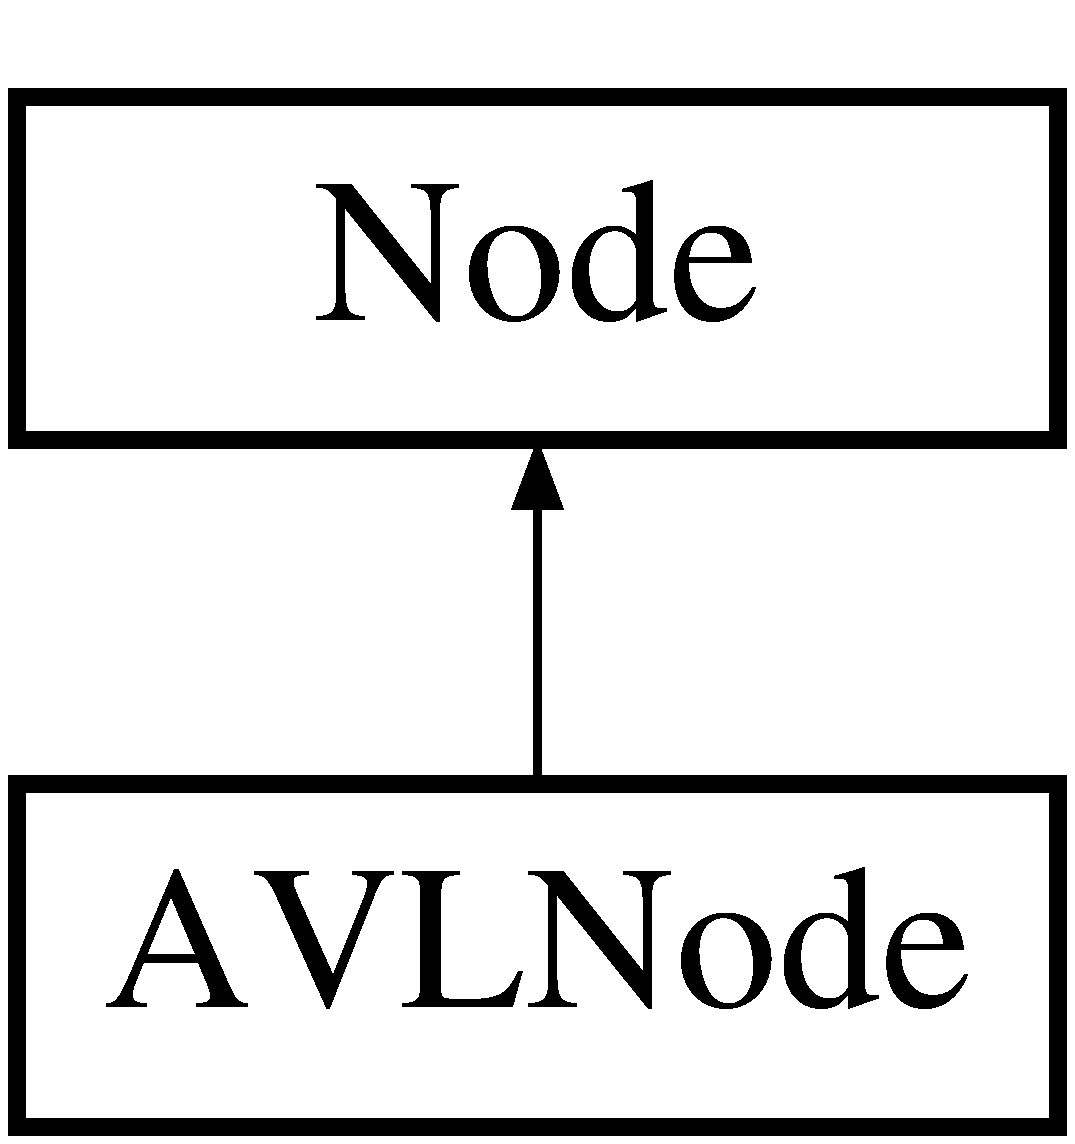
\includegraphics[height=2.000000cm]{class_a_v_l_node}
\end{center}
\end{figure}
\subsection*{Public Member Functions}
\begin{DoxyCompactItemize}
\item 
\hyperlink{class_a_v_l_node_ab4a77945ebefb824cb3d21a0f9f3a514}{A\+V\+L\+Node} ()
\item 
\hyperlink{class_a_v_l_node_af27568a3d6ad4d83e651a0cc0f4057aa}{A\+V\+L\+Node} (string, \hyperlink{class_page}{Page} $\ast$)
\item 
\hyperlink{class_a_v_l_node_ac549cb5dbe98c28f5335ceaf0f602111}{A\+V\+L\+Node} (string, \hyperlink{class_a_v_l_node}{A\+V\+L\+Node} $\ast$\&, \hyperlink{class_a_v_l_node}{A\+V\+L\+Node} $\ast$\&, \hyperlink{class_page}{Page} $\ast$)
\item 
\hyperlink{class_a_v_l_node_a5b3f7cdff426ea2ac77da59399e6a386}{$\sim$\+A\+V\+L\+Node} ()
\end{DoxyCompactItemize}
\subsection*{Friends}
\begin{DoxyCompactItemize}
\item 
class \hyperlink{class_a_v_l_node_abb802889854b7d6aebdc6c5a9f751b0e}{A\+V\+L\+Tree}
\end{DoxyCompactItemize}


\subsection{Detailed Description}
A\+V\+L \hyperlink{class_node}{Node} header file Sam Hunter and Morgan Monzingo node built for A\+V\+L tree 

\subsection{Constructor \& Destructor Documentation}
\hypertarget{class_a_v_l_node_ab4a77945ebefb824cb3d21a0f9f3a514}{}\index{A\+V\+L\+Node@{A\+V\+L\+Node}!A\+V\+L\+Node@{A\+V\+L\+Node}}
\index{A\+V\+L\+Node@{A\+V\+L\+Node}!A\+V\+L\+Node@{A\+V\+L\+Node}}
\subsubsection[{A\+V\+L\+Node}]{\setlength{\rightskip}{0pt plus 5cm}A\+V\+L\+Node\+::\+A\+V\+L\+Node (
\begin{DoxyParamCaption}
{}
\end{DoxyParamCaption}
)}\label{class_a_v_l_node_ab4a77945ebefb824cb3d21a0f9f3a514}
\hypertarget{class_a_v_l_node_af27568a3d6ad4d83e651a0cc0f4057aa}{}\index{A\+V\+L\+Node@{A\+V\+L\+Node}!A\+V\+L\+Node@{A\+V\+L\+Node}}
\index{A\+V\+L\+Node@{A\+V\+L\+Node}!A\+V\+L\+Node@{A\+V\+L\+Node}}
\subsubsection[{A\+V\+L\+Node}]{\setlength{\rightskip}{0pt plus 5cm}A\+V\+L\+Node\+::\+A\+V\+L\+Node (
\begin{DoxyParamCaption}
\item[{string}]{kw, }
\item[{{\bf Page} $\ast$}]{pg}
\end{DoxyParamCaption}
)}\label{class_a_v_l_node_af27568a3d6ad4d83e651a0cc0f4057aa}
\hypertarget{class_a_v_l_node_ac549cb5dbe98c28f5335ceaf0f602111}{}\index{A\+V\+L\+Node@{A\+V\+L\+Node}!A\+V\+L\+Node@{A\+V\+L\+Node}}
\index{A\+V\+L\+Node@{A\+V\+L\+Node}!A\+V\+L\+Node@{A\+V\+L\+Node}}
\subsubsection[{A\+V\+L\+Node}]{\setlength{\rightskip}{0pt plus 5cm}A\+V\+L\+Node\+::\+A\+V\+L\+Node (
\begin{DoxyParamCaption}
\item[{string}]{kw, }
\item[{{\bf A\+V\+L\+Node} $\ast$\&}]{rightnode, }
\item[{{\bf A\+V\+L\+Node} $\ast$\&}]{leftnode, }
\item[{{\bf Page} $\ast$}]{pg}
\end{DoxyParamCaption}
)}\label{class_a_v_l_node_ac549cb5dbe98c28f5335ceaf0f602111}
\hypertarget{class_a_v_l_node_a5b3f7cdff426ea2ac77da59399e6a386}{}\index{A\+V\+L\+Node@{A\+V\+L\+Node}!````~A\+V\+L\+Node@{$\sim$\+A\+V\+L\+Node}}
\index{````~A\+V\+L\+Node@{$\sim$\+A\+V\+L\+Node}!A\+V\+L\+Node@{A\+V\+L\+Node}}
\subsubsection[{$\sim$\+A\+V\+L\+Node}]{\setlength{\rightskip}{0pt plus 5cm}A\+V\+L\+Node\+::$\sim$\+A\+V\+L\+Node (
\begin{DoxyParamCaption}
{}
\end{DoxyParamCaption}
)}\label{class_a_v_l_node_a5b3f7cdff426ea2ac77da59399e6a386}


\subsection{Friends And Related Function Documentation}
\hypertarget{class_a_v_l_node_abb802889854b7d6aebdc6c5a9f751b0e}{}\index{A\+V\+L\+Node@{A\+V\+L\+Node}!A\+V\+L\+Tree@{A\+V\+L\+Tree}}
\index{A\+V\+L\+Tree@{A\+V\+L\+Tree}!A\+V\+L\+Node@{A\+V\+L\+Node}}
\subsubsection[{A\+V\+L\+Tree}]{\setlength{\rightskip}{0pt plus 5cm}friend class {\bf A\+V\+L\+Tree}\hspace{0.3cm}{\ttfamily [friend]}}\label{class_a_v_l_node_abb802889854b7d6aebdc6c5a9f751b0e}


The documentation for this class was generated from the following files\+:\begin{DoxyCompactItemize}
\item 
\hyperlink{_a_v_l_node_8h}{A\+V\+L\+Node.\+h}\item 
\hyperlink{_a_v_l_node_8cpp}{A\+V\+L\+Node.\+cpp}\end{DoxyCompactItemize}

\hypertarget{class_a_v_l_tree}{}\section{A\+V\+L\+Tree Class Reference}
\label{class_a_v_l_tree}\index{A\+V\+L\+Tree@{A\+V\+L\+Tree}}


{\ttfamily \#include $<$A\+V\+L\+Tree.\+h$>$}

Inheritance diagram for A\+V\+L\+Tree\+:\begin{figure}[H]
\begin{center}
\leavevmode
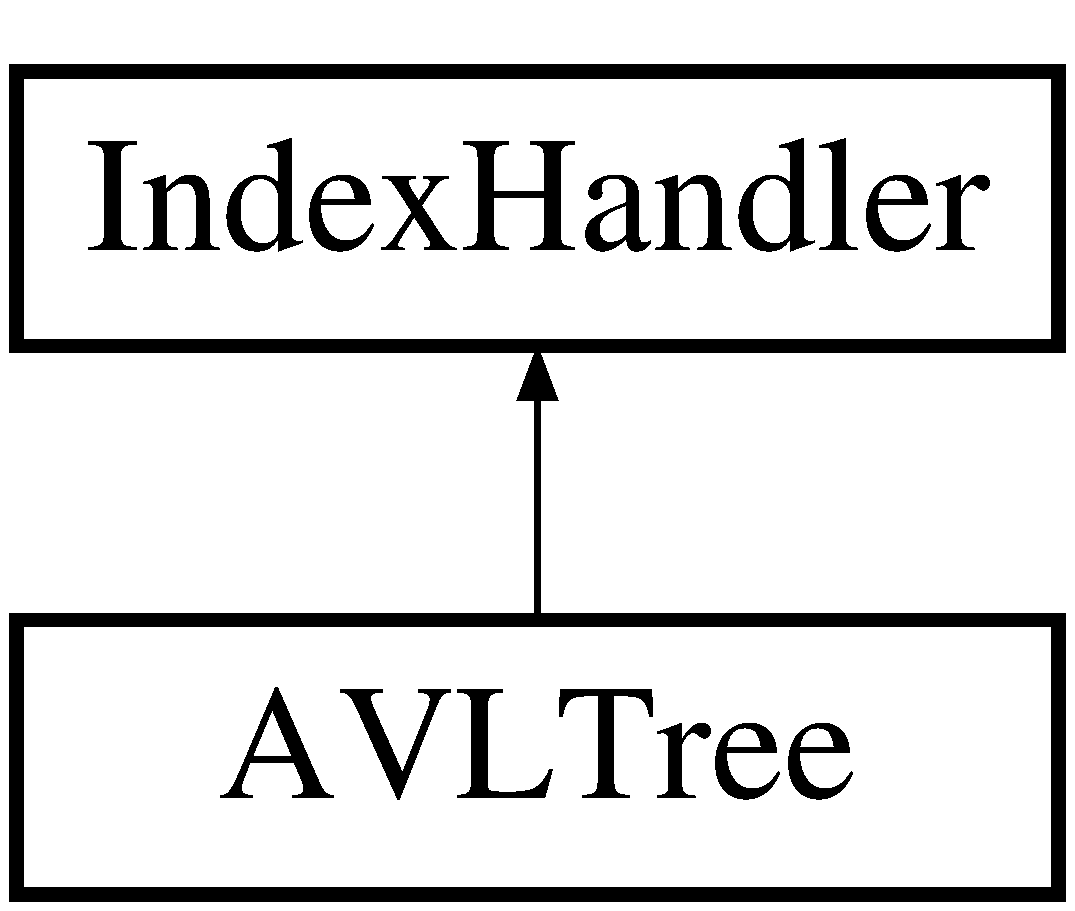
\includegraphics[height=2.000000cm]{class_a_v_l_tree}
\end{center}
\end{figure}
\subsection*{Public Member Functions}
\begin{DoxyCompactItemize}
\item 
\hyperlink{class_a_v_l_tree_a0915d328ebed07e11087692f17d80827}{A\+V\+L\+Tree} ()
\item 
\hyperlink{class_a_v_l_tree_af4a1d1be1b6301ba59c6e101c6efc6ba}{$\sim$\+A\+V\+L\+Tree} ()
\item 
void \hyperlink{class_a_v_l_tree_acc05c3c67a02da11ae973a01c37ae89e}{add\+To\+Index} (\hyperlink{class_page}{Page} $\ast$\&, string \&)
\item 
\hyperlink{class_a_v_l_node}{A\+V\+L\+Node} $\ast$\& \hyperlink{class_a_v_l_tree_a0e9a469764ef2056ffc1257ace172612}{insert} (string \&, \hyperlink{class_page}{Page} $\ast$\&, \hyperlink{class_a_v_l_node}{A\+V\+L\+Node} $\ast$\&)
\item 
\hyperlink{class_a_v_l_node}{A\+V\+L\+Node} $\ast$\& \hyperlink{class_a_v_l_tree_a6f77603032cfc0477eae2fc8944cec75}{balance} (\hyperlink{class_a_v_l_node}{A\+V\+L\+Node} $\ast$)
\item 
set$<$ \hyperlink{class_page}{Page} $\ast$ $>$ \hyperlink{class_a_v_l_tree_a7b6bc9d63cff082843ac1de050268f2d}{search\+Index} (string)
\item 
set$<$ \hyperlink{class_page}{Page} $\ast$ $>$ \hyperlink{class_a_v_l_tree_ac439d90d1a41fc1526e5882ba25f2a5b}{search} (string, \hyperlink{class_a_v_l_node}{A\+V\+L\+Node} $\ast$\&)
\item 
int \hyperlink{class_a_v_l_tree_ad3fb38e4b3f05d203dbc1d5c87be48b0}{height} (\hyperlink{class_a_v_l_node}{A\+V\+L\+Node} $\ast$)
\item 
int \hyperlink{class_a_v_l_tree_a4ba40b6b969fe541c840ac2e3ad1dd48}{difference} (\hyperlink{class_a_v_l_node}{A\+V\+L\+Node} $\ast$)
\item 
\hyperlink{class_a_v_l_node}{A\+V\+L\+Node} $\ast$\& \hyperlink{class_a_v_l_tree_ac861efd40852530f890f75af8adb05d3}{left\+Rotation} (\hyperlink{class_a_v_l_node}{A\+V\+L\+Node} $\ast$)
\begin{DoxyCompactList}\small\item\em rotations \end{DoxyCompactList}\item 
\hyperlink{class_a_v_l_node}{A\+V\+L\+Node} $\ast$\& \hyperlink{class_a_v_l_tree_a3d119fc1729d30c627b125f01dfa713f}{right\+Rotation} (\hyperlink{class_a_v_l_node}{A\+V\+L\+Node} $\ast$)
\item 
\hyperlink{class_a_v_l_node}{A\+V\+L\+Node} $\ast$\& \hyperlink{class_a_v_l_tree_aae25b3c2ba45785f14e6460f7da27a90}{double\+Left} (\hyperlink{class_a_v_l_node}{A\+V\+L\+Node} $\ast$)
\item 
\hyperlink{class_a_v_l_node}{A\+V\+L\+Node} $\ast$\& \hyperlink{class_a_v_l_tree_a52414545fb12fa95fd4b48410e32a90f}{double\+Right} (\hyperlink{class_a_v_l_node}{A\+V\+L\+Node} $\ast$)
\item 
void \hyperlink{class_a_v_l_tree_aaeb00045be61c381863d43526b4dffe1}{print\+Table} ()
\item 
void \hyperlink{class_a_v_l_tree_aadb95e92d5560738574ae428ae2df980}{display} (\hyperlink{class_a_v_l_node}{A\+V\+L\+Node} $\ast$, int)
\item 
void \hyperlink{class_a_v_l_tree_a3857ebba2ac14e0fd1ded8f1c6cb224c}{inorder} (\hyperlink{class_a_v_l_node}{A\+V\+L\+Node} $\ast$)
\item 
string \hyperlink{class_a_v_l_tree_a708b6398ea1771de3077ca39c4005cca}{get\+Class\+Type} ()
\end{DoxyCompactItemize}
\subsection*{Friends}
\begin{DoxyCompactItemize}
\item 
class \hyperlink{class_a_v_l_tree_aefbabd2f704298b266a25d1a555a63f0}{A\+V\+L\+Node}
\end{DoxyCompactItemize}


\subsection{Constructor \& Destructor Documentation}
\hypertarget{class_a_v_l_tree_a0915d328ebed07e11087692f17d80827}{}\index{A\+V\+L\+Tree@{A\+V\+L\+Tree}!A\+V\+L\+Tree@{A\+V\+L\+Tree}}
\index{A\+V\+L\+Tree@{A\+V\+L\+Tree}!A\+V\+L\+Tree@{A\+V\+L\+Tree}}
\subsubsection[{A\+V\+L\+Tree}]{\setlength{\rightskip}{0pt plus 5cm}A\+V\+L\+Tree\+::\+A\+V\+L\+Tree (
\begin{DoxyParamCaption}
{}
\end{DoxyParamCaption}
)}\label{class_a_v_l_tree_a0915d328ebed07e11087692f17d80827}
\hypertarget{class_a_v_l_tree_af4a1d1be1b6301ba59c6e101c6efc6ba}{}\index{A\+V\+L\+Tree@{A\+V\+L\+Tree}!````~A\+V\+L\+Tree@{$\sim$\+A\+V\+L\+Tree}}
\index{````~A\+V\+L\+Tree@{$\sim$\+A\+V\+L\+Tree}!A\+V\+L\+Tree@{A\+V\+L\+Tree}}
\subsubsection[{$\sim$\+A\+V\+L\+Tree}]{\setlength{\rightskip}{0pt plus 5cm}A\+V\+L\+Tree\+::$\sim$\+A\+V\+L\+Tree (
\begin{DoxyParamCaption}
{}
\end{DoxyParamCaption}
)}\label{class_a_v_l_tree_af4a1d1be1b6301ba59c6e101c6efc6ba}


\subsection{Member Function Documentation}
\hypertarget{class_a_v_l_tree_acc05c3c67a02da11ae973a01c37ae89e}{}\index{A\+V\+L\+Tree@{A\+V\+L\+Tree}!add\+To\+Index@{add\+To\+Index}}
\index{add\+To\+Index@{add\+To\+Index}!A\+V\+L\+Tree@{A\+V\+L\+Tree}}
\subsubsection[{add\+To\+Index}]{\setlength{\rightskip}{0pt plus 5cm}void A\+V\+L\+Tree\+::add\+To\+Index (
\begin{DoxyParamCaption}
\item[{{\bf Page} $\ast$\&}]{pg, }
\item[{string \&}]{kw}
\end{DoxyParamCaption}
)}\label{class_a_v_l_tree_acc05c3c67a02da11ae973a01c37ae89e}
\hypertarget{class_a_v_l_tree_a6f77603032cfc0477eae2fc8944cec75}{}\index{A\+V\+L\+Tree@{A\+V\+L\+Tree}!balance@{balance}}
\index{balance@{balance}!A\+V\+L\+Tree@{A\+V\+L\+Tree}}
\subsubsection[{balance}]{\setlength{\rightskip}{0pt plus 5cm}{\bf A\+V\+L\+Node} $\ast$\& A\+V\+L\+Tree\+::balance (
\begin{DoxyParamCaption}
\item[{{\bf A\+V\+L\+Node} $\ast$}]{avlnode}
\end{DoxyParamCaption}
)}\label{class_a_v_l_tree_a6f77603032cfc0477eae2fc8944cec75}
\hypertarget{class_a_v_l_tree_a4ba40b6b969fe541c840ac2e3ad1dd48}{}\index{A\+V\+L\+Tree@{A\+V\+L\+Tree}!difference@{difference}}
\index{difference@{difference}!A\+V\+L\+Tree@{A\+V\+L\+Tree}}
\subsubsection[{difference}]{\setlength{\rightskip}{0pt plus 5cm}int A\+V\+L\+Tree\+::difference (
\begin{DoxyParamCaption}
\item[{{\bf A\+V\+L\+Node} $\ast$}]{avlnode}
\end{DoxyParamCaption}
)}\label{class_a_v_l_tree_a4ba40b6b969fe541c840ac2e3ad1dd48}
\hypertarget{class_a_v_l_tree_aadb95e92d5560738574ae428ae2df980}{}\index{A\+V\+L\+Tree@{A\+V\+L\+Tree}!display@{display}}
\index{display@{display}!A\+V\+L\+Tree@{A\+V\+L\+Tree}}
\subsubsection[{display}]{\setlength{\rightskip}{0pt plus 5cm}void A\+V\+L\+Tree\+::display (
\begin{DoxyParamCaption}
\item[{{\bf A\+V\+L\+Node} $\ast$}]{ptr, }
\item[{int}]{level}
\end{DoxyParamCaption}
)}\label{class_a_v_l_tree_aadb95e92d5560738574ae428ae2df980}
\hypertarget{class_a_v_l_tree_aae25b3c2ba45785f14e6460f7da27a90}{}\index{A\+V\+L\+Tree@{A\+V\+L\+Tree}!double\+Left@{double\+Left}}
\index{double\+Left@{double\+Left}!A\+V\+L\+Tree@{A\+V\+L\+Tree}}
\subsubsection[{double\+Left}]{\setlength{\rightskip}{0pt plus 5cm}{\bf A\+V\+L\+Node} $\ast$\& A\+V\+L\+Tree\+::double\+Left (
\begin{DoxyParamCaption}
\item[{{\bf A\+V\+L\+Node} $\ast$}]{avlnode}
\end{DoxyParamCaption}
)}\label{class_a_v_l_tree_aae25b3c2ba45785f14e6460f7da27a90}
\hypertarget{class_a_v_l_tree_a52414545fb12fa95fd4b48410e32a90f}{}\index{A\+V\+L\+Tree@{A\+V\+L\+Tree}!double\+Right@{double\+Right}}
\index{double\+Right@{double\+Right}!A\+V\+L\+Tree@{A\+V\+L\+Tree}}
\subsubsection[{double\+Right}]{\setlength{\rightskip}{0pt plus 5cm}{\bf A\+V\+L\+Node} $\ast$\& A\+V\+L\+Tree\+::double\+Right (
\begin{DoxyParamCaption}
\item[{{\bf A\+V\+L\+Node} $\ast$}]{avlnode}
\end{DoxyParamCaption}
)}\label{class_a_v_l_tree_a52414545fb12fa95fd4b48410e32a90f}
\hypertarget{class_a_v_l_tree_a708b6398ea1771de3077ca39c4005cca}{}\index{A\+V\+L\+Tree@{A\+V\+L\+Tree}!get\+Class\+Type@{get\+Class\+Type}}
\index{get\+Class\+Type@{get\+Class\+Type}!A\+V\+L\+Tree@{A\+V\+L\+Tree}}
\subsubsection[{get\+Class\+Type}]{\setlength{\rightskip}{0pt plus 5cm}string A\+V\+L\+Tree\+::get\+Class\+Type (
\begin{DoxyParamCaption}
{}
\end{DoxyParamCaption}
)\hspace{0.3cm}{\ttfamily [virtual]}}\label{class_a_v_l_tree_a708b6398ea1771de3077ca39c4005cca}


Implements \hyperlink{class_index_handler_aaeb0f250516fbc93936efec2c3f21359}{Index\+Handler}.

\hypertarget{class_a_v_l_tree_ad3fb38e4b3f05d203dbc1d5c87be48b0}{}\index{A\+V\+L\+Tree@{A\+V\+L\+Tree}!height@{height}}
\index{height@{height}!A\+V\+L\+Tree@{A\+V\+L\+Tree}}
\subsubsection[{height}]{\setlength{\rightskip}{0pt plus 5cm}int A\+V\+L\+Tree\+::height (
\begin{DoxyParamCaption}
\item[{{\bf A\+V\+L\+Node} $\ast$}]{avlnode}
\end{DoxyParamCaption}
)}\label{class_a_v_l_tree_ad3fb38e4b3f05d203dbc1d5c87be48b0}
\hypertarget{class_a_v_l_tree_a3857ebba2ac14e0fd1ded8f1c6cb224c}{}\index{A\+V\+L\+Tree@{A\+V\+L\+Tree}!inorder@{inorder}}
\index{inorder@{inorder}!A\+V\+L\+Tree@{A\+V\+L\+Tree}}
\subsubsection[{inorder}]{\setlength{\rightskip}{0pt plus 5cm}void A\+V\+L\+Tree\+::inorder (
\begin{DoxyParamCaption}
\item[{{\bf A\+V\+L\+Node} $\ast$}]{temp}
\end{DoxyParamCaption}
)}\label{class_a_v_l_tree_a3857ebba2ac14e0fd1ded8f1c6cb224c}
\hypertarget{class_a_v_l_tree_a0e9a469764ef2056ffc1257ace172612}{}\index{A\+V\+L\+Tree@{A\+V\+L\+Tree}!insert@{insert}}
\index{insert@{insert}!A\+V\+L\+Tree@{A\+V\+L\+Tree}}
\subsubsection[{insert}]{\setlength{\rightskip}{0pt plus 5cm}{\bf A\+V\+L\+Node} $\ast$\& A\+V\+L\+Tree\+::insert (
\begin{DoxyParamCaption}
\item[{string \&}]{kw, }
\item[{{\bf Page} $\ast$\&}]{pg, }
\item[{{\bf A\+V\+L\+Node} $\ast$\&}]{avlnode}
\end{DoxyParamCaption}
)}\label{class_a_v_l_tree_a0e9a469764ef2056ffc1257ace172612}
\hypertarget{class_a_v_l_tree_ac861efd40852530f890f75af8adb05d3}{}\index{A\+V\+L\+Tree@{A\+V\+L\+Tree}!left\+Rotation@{left\+Rotation}}
\index{left\+Rotation@{left\+Rotation}!A\+V\+L\+Tree@{A\+V\+L\+Tree}}
\subsubsection[{left\+Rotation}]{\setlength{\rightskip}{0pt plus 5cm}{\bf A\+V\+L\+Node} $\ast$\& A\+V\+L\+Tree\+::left\+Rotation (
\begin{DoxyParamCaption}
\item[{{\bf A\+V\+L\+Node} $\ast$}]{avlnode}
\end{DoxyParamCaption}
)}\label{class_a_v_l_tree_ac861efd40852530f890f75af8adb05d3}


rotations 

\hypertarget{class_a_v_l_tree_aaeb00045be61c381863d43526b4dffe1}{}\index{A\+V\+L\+Tree@{A\+V\+L\+Tree}!print\+Table@{print\+Table}}
\index{print\+Table@{print\+Table}!A\+V\+L\+Tree@{A\+V\+L\+Tree}}
\subsubsection[{print\+Table}]{\setlength{\rightskip}{0pt plus 5cm}void A\+V\+L\+Tree\+::print\+Table (
\begin{DoxyParamCaption}
{}
\end{DoxyParamCaption}
)\hspace{0.3cm}{\ttfamily [virtual]}}\label{class_a_v_l_tree_aaeb00045be61c381863d43526b4dffe1}


Implements \hyperlink{class_index_handler_a036ccca02cb734711a1e6a50b09a2b1f}{Index\+Handler}.

\hypertarget{class_a_v_l_tree_a3d119fc1729d30c627b125f01dfa713f}{}\index{A\+V\+L\+Tree@{A\+V\+L\+Tree}!right\+Rotation@{right\+Rotation}}
\index{right\+Rotation@{right\+Rotation}!A\+V\+L\+Tree@{A\+V\+L\+Tree}}
\subsubsection[{right\+Rotation}]{\setlength{\rightskip}{0pt plus 5cm}{\bf A\+V\+L\+Node} $\ast$\& A\+V\+L\+Tree\+::right\+Rotation (
\begin{DoxyParamCaption}
\item[{{\bf A\+V\+L\+Node} $\ast$}]{avlnode}
\end{DoxyParamCaption}
)}\label{class_a_v_l_tree_a3d119fc1729d30c627b125f01dfa713f}
\hypertarget{class_a_v_l_tree_ac439d90d1a41fc1526e5882ba25f2a5b}{}\index{A\+V\+L\+Tree@{A\+V\+L\+Tree}!search@{search}}
\index{search@{search}!A\+V\+L\+Tree@{A\+V\+L\+Tree}}
\subsubsection[{search}]{\setlength{\rightskip}{0pt plus 5cm}set$<$ {\bf Page} $\ast$ $>$ A\+V\+L\+Tree\+::search (
\begin{DoxyParamCaption}
\item[{string}]{search\+\_\+string, }
\item[{{\bf A\+V\+L\+Node} $\ast$\&}]{root}
\end{DoxyParamCaption}
)}\label{class_a_v_l_tree_ac439d90d1a41fc1526e5882ba25f2a5b}
\hypertarget{class_a_v_l_tree_a7b6bc9d63cff082843ac1de050268f2d}{}\index{A\+V\+L\+Tree@{A\+V\+L\+Tree}!search\+Index@{search\+Index}}
\index{search\+Index@{search\+Index}!A\+V\+L\+Tree@{A\+V\+L\+Tree}}
\subsubsection[{search\+Index}]{\setlength{\rightskip}{0pt plus 5cm}set$<$ {\bf Page} $\ast$ $>$ A\+V\+L\+Tree\+::search\+Index (
\begin{DoxyParamCaption}
\item[{string}]{search\+\_\+term}
\end{DoxyParamCaption}
)}\label{class_a_v_l_tree_a7b6bc9d63cff082843ac1de050268f2d}


\subsection{Friends And Related Function Documentation}
\hypertarget{class_a_v_l_tree_aefbabd2f704298b266a25d1a555a63f0}{}\index{A\+V\+L\+Tree@{A\+V\+L\+Tree}!A\+V\+L\+Node@{A\+V\+L\+Node}}
\index{A\+V\+L\+Node@{A\+V\+L\+Node}!A\+V\+L\+Tree@{A\+V\+L\+Tree}}
\subsubsection[{A\+V\+L\+Node}]{\setlength{\rightskip}{0pt plus 5cm}friend class {\bf A\+V\+L\+Node}\hspace{0.3cm}{\ttfamily [friend]}}\label{class_a_v_l_tree_aefbabd2f704298b266a25d1a555a63f0}


The documentation for this class was generated from the following files\+:\begin{DoxyCompactItemize}
\item 
\hyperlink{_a_v_l_tree_8h}{A\+V\+L\+Tree.\+h}\item 
\hyperlink{_a_v_l_tree_8cpp}{A\+V\+L\+Tree.\+cpp}\end{DoxyCompactItemize}

\hypertarget{classbackup__variable}{\section{backup\+\_\+variable$<$ T $>$ Class Template Reference}
\label{classbackup__variable}\index{backup\+\_\+variable$<$ T $>$@{backup\+\_\+variable$<$ T $>$}}
}
\subsection*{Public Member Functions}
\begin{DoxyCompactItemize}
\item 
\hypertarget{classbackup__variable_a5ffb4ce0ce0f679135ce70d8683a9182}{{\bfseries backup\+\_\+variable} (const T \&value)}\label{classbackup__variable_a5ffb4ce0ce0f679135ce70d8683a9182}

\item 
\hypertarget{classbackup__variable_ae4c8c3147d8a341eb268f7b2332098d6}{void {\bfseries operator=} (const T \&value)}\label{classbackup__variable_ae4c8c3147d8a341eb268f7b2332098d6}

\item 
\hypertarget{classbackup__variable_aec3207431e35f74efa6fe2af77ec734d}{bool {\bfseries operator==} (const T \&value) const }\label{classbackup__variable_aec3207431e35f74efa6fe2af77ec734d}

\item 
\hypertarget{classbackup__variable_af6d27d4c48c46816a5f82343609b24db}{bool {\bfseries operator$<$} (const T \&value) const }\label{classbackup__variable_af6d27d4c48c46816a5f82343609b24db}

\item 
\hypertarget{classbackup__variable_a60de5d54f02e5d862ae851ab773830db}{bool {\bfseries operator$<$=} (const T \&value) const }\label{classbackup__variable_a60de5d54f02e5d862ae851ab773830db}

\item 
\hypertarget{classbackup__variable_a1956d30f9a5124527ac9d52821ce9d72}{bool {\bfseries operator$>$} (const T \&value) const }\label{classbackup__variable_a1956d30f9a5124527ac9d52821ce9d72}

\item 
\hypertarget{classbackup__variable_a0b749c6e3c84c43d094d1ba50d1a2323}{bool {\bfseries operator$>$=} (const T \&value) const }\label{classbackup__variable_a0b749c6e3c84c43d094d1ba50d1a2323}

\item 
\hypertarget{classbackup__variable_a1ae3f1fcce3725da51aab2879c523a09}{void {\bfseries operator+} (const T \&value)}\label{classbackup__variable_a1ae3f1fcce3725da51aab2879c523a09}

\item 
\hypertarget{classbackup__variable_a4b5753702dbfdaf23f9eb8b210ed80a2}{void {\bfseries operator+=} (const T \&value)}\label{classbackup__variable_a4b5753702dbfdaf23f9eb8b210ed80a2}

\item 
\hypertarget{classbackup__variable_abc321dce84d827d20d69b96653049739}{void {\bfseries operator-\/} (const T \&value)}\label{classbackup__variable_abc321dce84d827d20d69b96653049739}

\item 
\hypertarget{classbackup__variable_adc890d1d8539089e654280bf18e76034}{void {\bfseries operator-\/=} (const T \&value)}\label{classbackup__variable_adc890d1d8539089e654280bf18e76034}

\item 
\hypertarget{classbackup__variable_acba460a7693d0db536d7f9768ab6cf67}{{\bfseries operator const T} () const }\label{classbackup__variable_acba460a7693d0db536d7f9768ab6cf67}

\item 
\hypertarget{classbackup__variable_a61a6e2eee207d52e8f80f23595615627}{T $\ast$ {\bfseries operator\&} ()}\label{classbackup__variable_a61a6e2eee207d52e8f80f23595615627}

\item 
\hypertarget{classbackup__variable_a1239b41350b1570e28479647525f9846}{T {\bfseries get\+\_\+value} () const }\label{classbackup__variable_a1239b41350b1570e28479647525f9846}

\item 
\hypertarget{classbackup__variable_a4d062c1afac850f6e965ccf6ebdca951}{bool {\bfseries has\+\_\+changed} () const }\label{classbackup__variable_a4d062c1afac850f6e965ccf6ebdca951}

\end{DoxyCompactItemize}


The documentation for this class was generated from the following file\+:\begin{DoxyCompactItemize}
\item 
utilities.\+h\end{DoxyCompactItemize}

\hypertarget{class_document_parser}{\section{Document\+Parser Class Reference}
\label{class_document_parser}\index{Document\+Parser@{Document\+Parser}}
}
\subsection*{Public Member Functions}
\begin{DoxyCompactItemize}
\item 
\hypertarget{class_document_parser_a40fc3f32cbe2d6f4f978caa42ee509d6}{void {\bfseries parse\+Drive} (string, \hyperlink{class_index_handler}{Index\+Handler} $\ast$\&)}\label{class_document_parser_a40fc3f32cbe2d6f4f978caa42ee509d6}

\item 
\hypertarget{class_document_parser_ae132955b8118c74df2705defd1fe856b}{void {\bfseries send\+To\+Index} (\hyperlink{class_page}{Page} $\ast$)}\label{class_document_parser_ae132955b8118c74df2705defd1fe856b}

\item 
\hypertarget{class_document_parser_a7ca97302ad273efde7f33163ab9e78dc}{void {\bfseries write\+To\+Structure} (\hyperlink{class_index_handler}{Index\+Handler} $\ast$\&, int start\+Index=0)}\label{class_document_parser_a7ca97302ad273efde7f33163ab9e78dc}

\item 
\hypertarget{class_document_parser_a8f07107cbe76401f9db73dbf9cae7a5f}{void {\bfseries save\+Index} ()}\label{class_document_parser_a8f07107cbe76401f9db73dbf9cae7a5f}

\item 
\hypertarget{class_document_parser_a8046232e6026fb59d3052426e7ed7a58}{void {\bfseries read\+In\+Parsed\+File} (\hyperlink{class_index_handler}{Index\+Handler} $\ast$\&)}\label{class_document_parser_a8046232e6026fb59d3052426e7ed7a58}

\item 
\hypertarget{class_document_parser_a23dd86d1fb040662e97845d2499e5ae1}{int {\bfseries get\+Collection\+Size} ()}\label{class_document_parser_a23dd86d1fb040662e97845d2499e5ae1}

\end{DoxyCompactItemize}


The documentation for this class was generated from the following files\+:\begin{DoxyCompactItemize}
\item 
Document\+Parser.\+h\item 
Document\+Parser.\+cpp\end{DoxyCompactItemize}

\hypertarget{classstemming_1_1english__stem}{\section{stemming\+:\+:english\+\_\+stem$<$ string\+\_\+type\+T $>$ Class Template Reference}
\label{classstemming_1_1english__stem}\index{stemming\+::english\+\_\+stem$<$ string\+\_\+type\+T $>$@{stemming\+::english\+\_\+stem$<$ string\+\_\+type\+T $>$}}
}


{\ttfamily \#include $<$english\+\_\+stem.\+h$>$}

Inheritance diagram for stemming\+:\+:english\+\_\+stem$<$ string\+\_\+type\+T $>$\+:\begin{figure}[H]
\begin{center}
\leavevmode
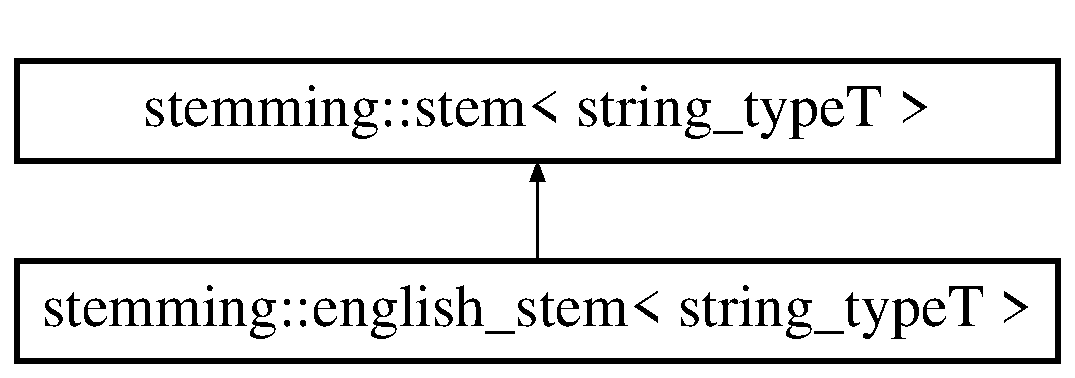
\includegraphics[height=2.000000cm]{classstemming_1_1english__stem}
\end{center}
\end{figure}
\subsection*{Public Member Functions}
\begin{DoxyCompactItemize}
\item 
void \hyperlink{classstemming_1_1english__stem_a8163a8cc4186b749665d616cbf11c492}{operator()} (string\+\_\+type\+T \&text)
\end{DoxyCompactItemize}
\subsection*{Additional Inherited Members}


\subsection{Detailed Description}
\subsubsection*{template$<$typename string\+\_\+type\+T = std\+::wstring$>$class stemming\+::english\+\_\+stem$<$ string\+\_\+type\+T $>$}

Overview

I have made more than one attempt to improve the structure of the Porter algorithm by making it follow the pattern of ending removal of the Romance language stemmers. It is not hard to see why one should want to do this\+: step 1b of the Porter stemmer removes ed and ing, which are i-\/suffixes ($\ast$) attached to verbs. If these suffixes are removed, there should be no need to remove d-\/suffixes which are not verbal, although it will try to do so. This seems to be a deficiency in the Porter stemmer, not shared by the Romance stemmers. Again, the divisions between steps 2, 3 and 4 seem rather arbitrary, and are not found in the Romance stemmers.

Nevertheless, these attempts at improvement have been abandoned. They seem to lead to a more complicated algorithm with no very obvious improvements. A reason for not taking note of the outcome of step 1b may be that English endings do not determine word categories quite as strongly as endings in the Romance languages. For example, condition and position in French have to be nouns, but in English they can be verbs as well as nouns,

We are all conditioned by advertising They are positioning themselves differently today

A possible reason for having separate steps 2, 3 and 4 is that d-\/suffix combinations in English are quite complex, a point which has been made elsewhere.

But it is hardly surprising that after twenty years of use of the Porter stemmer, certain improvements do suggest themselves, and a new algorithm for English is therefore offered here. (It could be called the 'Porter2' stemmer to distinguish it from the Porter stemmer, from which it derives.) The changes are not so very extensive\+: (1) terminating y is changed to i rather less often, (2) suffix us does not lose its s, (3) a few additional suffixes are included for removal, including (4) suffix ly. In addition, a small list of exceptional forms is included. In December 2001 there were two further adjustments\+: (5) Steps 5a and 5b of the old Porter stemmer were combined into a single step. This means that undoubling final ll is not done with removal of final e. (6) In Step 3 ative is removed only when in region R2.

To begin with, here is the basic algorithm without reference to the exceptional forms. An exact comparison with the Porter algorithm needs to be done quite carefully if done at all. Here we indicate by $\ast$ points of departure, and by + additional features. In the sample vocabulary, Porter and Porter2 stem slightly under 5\% of words to different forms.

Dr. Martin Porter

Define a vowel as one of -\/a e i o u y

Define a double as one of -\/bb dd ff gg mm nn pp rr tt

Define a valid li-\/ending as one of -\/c d e g h k m n r t

Define a short syllable in a word as either (a) a vowel followed by a non-\/vowel other than w, x or Y and preceded by a non-\/vowel, or $\ast$ (b) a vowel at the beginning of the word followed by a non-\/vowel.

So rap, trap, entrap end with a short syllable, and ow, on, at are classed as short syllables. But uproot, bestow, disturb do not end with a short syllable.

A word is called short if it consists of a short syllable preceded by zero or more consonants. R1 is the region after the first non-\/vowel following a vowel, or the end of the word if there is no such non-\/vowel. R2 is the region after the first non-\/vowel following a vowel in R1, or the end of the word if there is no such non-\/vowel. If the word has two letters or less, leave it as it is. Otherwise, do each of the following operations, Set initial y, or y after a vowel, to Y, and then establish the regions R1 and R2. 

\subsection{Member Function Documentation}
\hypertarget{classstemming_1_1english__stem_a8163a8cc4186b749665d616cbf11c492}{\index{stemming\+::english\+\_\+stem@{stemming\+::english\+\_\+stem}!operator()@{operator()}}
\index{operator()@{operator()}!stemming\+::english\+\_\+stem@{stemming\+::english\+\_\+stem}}
\subsubsection[{operator()}]{\setlength{\rightskip}{0pt plus 5cm}template$<$typename string\+\_\+type\+T  = std\+::wstring$>$ void {\bf stemming\+::english\+\_\+stem}$<$ string\+\_\+type\+T $>$\+::operator() (
\begin{DoxyParamCaption}
\item[{string\+\_\+type\+T \&}]{text}
\end{DoxyParamCaption}
)\hspace{0.3cm}{\ttfamily [inline]}}}\label{classstemming_1_1english__stem_a8163a8cc4186b749665d616cbf11c492}

\begin{DoxyParams}{Parameters}
{\em text} & string to stem \\
\hline
\end{DoxyParams}


The documentation for this class was generated from the following file\+:\begin{DoxyCompactItemize}
\item 
english\+\_\+stem.\+h\end{DoxyCompactItemize}

\hypertarget{classstring__util_1_1equal__string__i__compare}{\section{string\+\_\+util\+:\+:equal\+\_\+string\+\_\+i\+\_\+compare$<$ T $>$ Class Template Reference}
\label{classstring__util_1_1equal__string__i__compare}\index{string\+\_\+util\+::equal\+\_\+string\+\_\+i\+\_\+compare$<$ T $>$@{string\+\_\+util\+::equal\+\_\+string\+\_\+i\+\_\+compare$<$ T $>$}}
}
Inheritance diagram for string\+\_\+util\+:\+:equal\+\_\+string\+\_\+i\+\_\+compare$<$ T $>$\+:\begin{figure}[H]
\begin{center}
\leavevmode
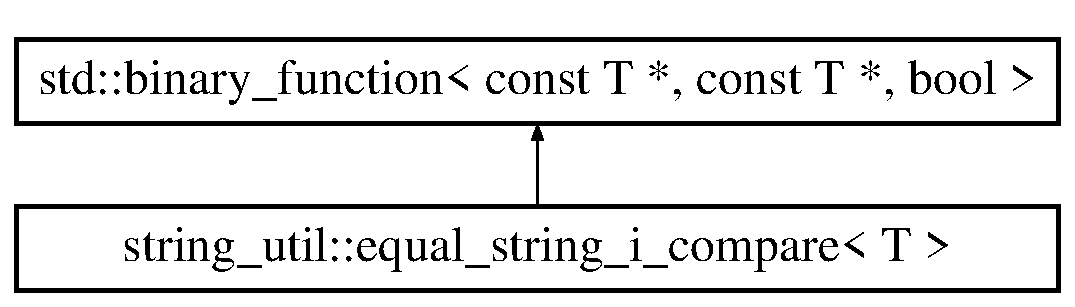
\includegraphics[height=2.000000cm]{classstring__util_1_1equal__string__i__compare}
\end{center}
\end{figure}
\subsection*{Public Member Functions}
\begin{DoxyCompactItemize}
\item 
\hypertarget{classstring__util_1_1equal__string__i__compare_af8c94159bbb8903c7cf7b71941a7d2bc}{bool {\bfseries operator()} (const T $\ast$a\+\_\+, const T $\ast$b\+\_\+) const }\label{classstring__util_1_1equal__string__i__compare_af8c94159bbb8903c7cf7b71941a7d2bc}

\end{DoxyCompactItemize}


The documentation for this class was generated from the following file\+:\begin{DoxyCompactItemize}
\item 
string\+\_\+util.\+h\end{DoxyCompactItemize}

\hypertarget{classeven}{\section{even$<$ T $>$ Class Template Reference}
\label{classeven}\index{even$<$ T $>$@{even$<$ T $>$}}
}
Inheritance diagram for even$<$ T $>$\+:\begin{figure}[H]
\begin{center}
\leavevmode
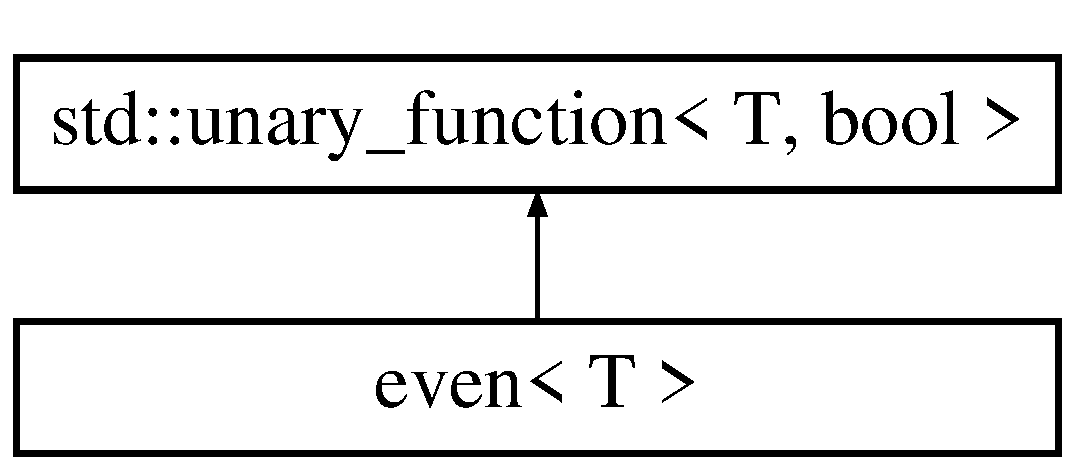
\includegraphics[height=2.000000cm]{classeven}
\end{center}
\end{figure}
\subsection*{Public Member Functions}
\begin{DoxyCompactItemize}
\item 
\hypertarget{classeven_a08c10e28d676fb0d25ca1fc214fcf73b}{bool {\bfseries operator()} (const T \&val) const }\label{classeven_a08c10e28d676fb0d25ca1fc214fcf73b}

\end{DoxyCompactItemize}


The documentation for this class was generated from the following file\+:\begin{DoxyCompactItemize}
\item 
utilities.\+h\end{DoxyCompactItemize}

\hypertarget{class_hash_node}{\section{Hash\+Node Class Reference}
\label{class_hash_node}\index{Hash\+Node@{Hash\+Node}}
}
Inheritance diagram for Hash\+Node\+:\begin{figure}[H]
\begin{center}
\leavevmode
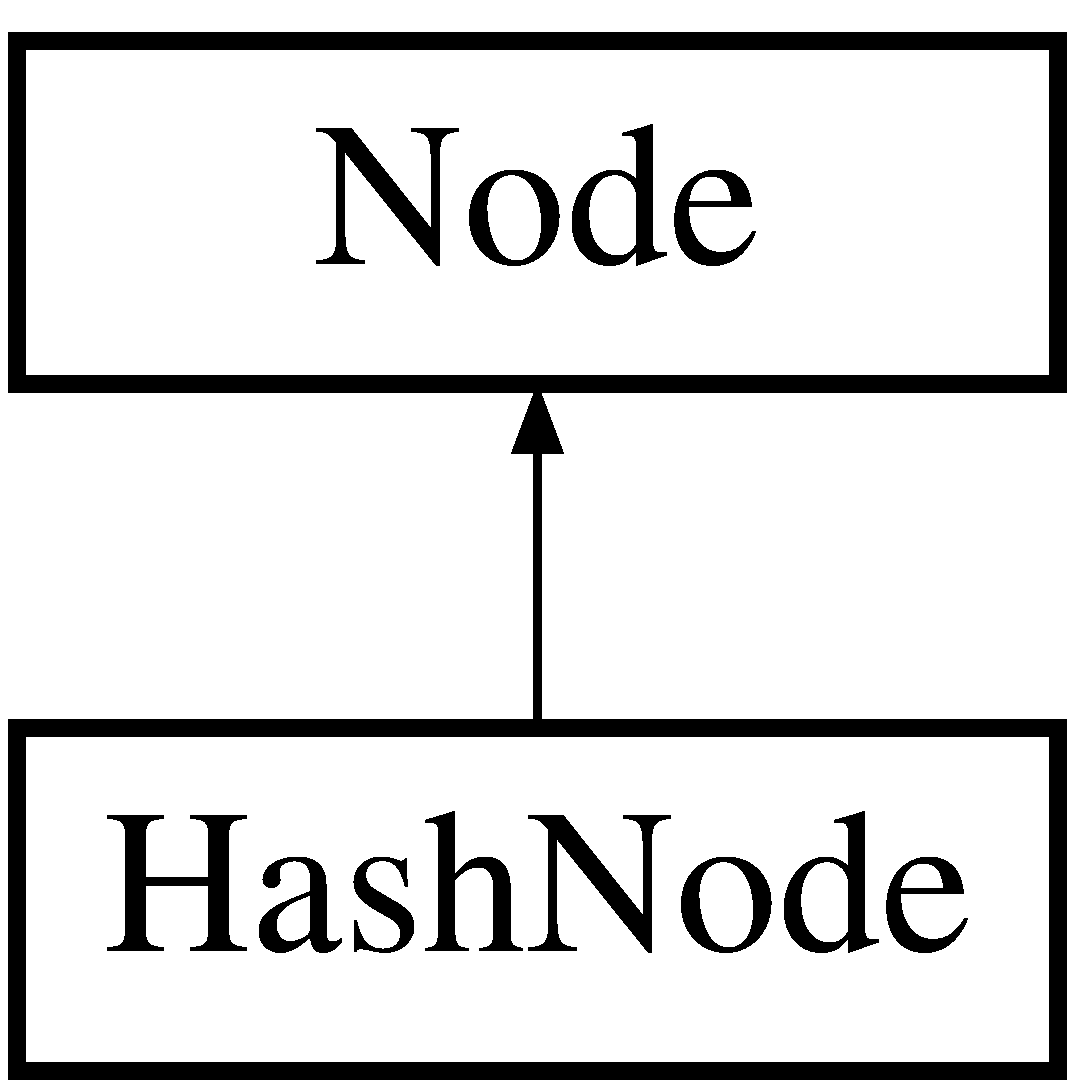
\includegraphics[height=2.000000cm]{class_hash_node}
\end{center}
\end{figure}
\subsection*{Public Member Functions}
\begin{DoxyCompactItemize}
\item 
\hypertarget{class_hash_node_af85be330cc34bb55f26041c7224b5b25}{{\bfseries Hash\+Node} (\hyperlink{class_node}{Node} $\ast$\&other)}\label{class_hash_node_af85be330cc34bb55f26041c7224b5b25}

\item 
\hypertarget{class_hash_node_ae3a3c1f03c060e03cc01ef81aae2c734}{\hyperlink{class_hash_node}{Hash\+Node} $\ast$ {\bfseries get\+Next\+Hash\+Node} ()}\label{class_hash_node_ae3a3c1f03c060e03cc01ef81aae2c734}

\item 
\hypertarget{class_hash_node_a0711b28c4cbdb8a21e6df486896081b3}{void {\bfseries set\+Next\+Hash\+Node} (\hyperlink{class_hash_node}{Hash\+Node} $\ast$)}\label{class_hash_node_a0711b28c4cbdb8a21e6df486896081b3}

\end{DoxyCompactItemize}
\subsection*{Friends}
\begin{DoxyCompactItemize}
\item 
\hypertarget{class_hash_node_a574ea806a7ec4e2f0fa54ed7da67b628}{class {\bfseries Hash\+Table}}\label{class_hash_node_a574ea806a7ec4e2f0fa54ed7da67b628}

\end{DoxyCompactItemize}


The documentation for this class was generated from the following files\+:\begin{DoxyCompactItemize}
\item 
Hash\+Node.\+h\item 
Hash\+Node.\+cpp\end{DoxyCompactItemize}

\hypertarget{class_hash_table}{\section{Hash\+Table Class Reference}
\label{class_hash_table}\index{Hash\+Table@{Hash\+Table}}
}
Inheritance diagram for Hash\+Table\+:\begin{figure}[H]
\begin{center}
\leavevmode
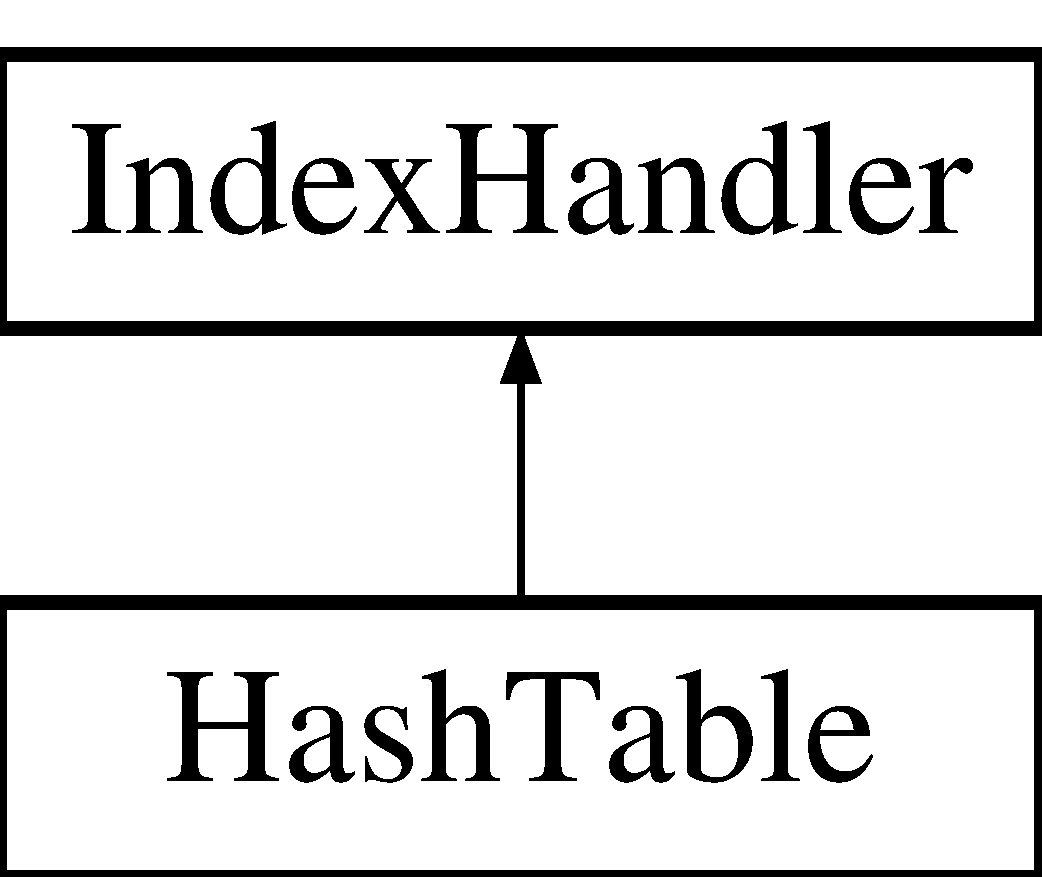
\includegraphics[height=2.000000cm]{class_hash_table}
\end{center}
\end{figure}
\subsection*{Public Member Functions}
\begin{DoxyCompactItemize}
\item 
\hypertarget{class_hash_table_aaa6417f06baad4f297d098dc7393e48b}{void {\bfseries add\+To\+Index} (\hyperlink{class_page}{Page} $\ast$\&, string \&)}\label{class_hash_table_aaa6417f06baad4f297d098dc7393e48b}

\item 
\hypertarget{class_hash_table_ab50be186df67a5621694cb2f692de3fa}{void {\bfseries print\+Table} ()}\label{class_hash_table_ab50be186df67a5621694cb2f692de3fa}

\item 
\hypertarget{class_hash_table_a838109ea89fa1b80908aee6838d96ad1}{set$<$ \hyperlink{class_page}{Page} $\ast$ $>$ {\bfseries search\+Index} (string)}\label{class_hash_table_a838109ea89fa1b80908aee6838d96ad1}

\item 
\hypertarget{class_hash_table_ad42a8eb156c387de2645ca1276ea412a}{void {\bfseries save\+Index} ()}\label{class_hash_table_ad42a8eb156c387de2645ca1276ea412a}

\item 
\hypertarget{class_hash_table_ab5a5fca28242a0733cb95e0729d94761}{string {\bfseries get\+Class\+Type} ()}\label{class_hash_table_ab5a5fca28242a0733cb95e0729d94761}

\item 
\hypertarget{class_hash_table_acf96b4d4e320ab83fbeed1578a415be8}{void {\bfseries destroy\+Structure} ()}\label{class_hash_table_acf96b4d4e320ab83fbeed1578a415be8}

\end{DoxyCompactItemize}


The documentation for this class was generated from the following files\+:\begin{DoxyCompactItemize}
\item 
Hash\+Table.\+h\item 
Hash\+Table.\+cpp\end{DoxyCompactItemize}

\hypertarget{class_index_handler}{}\section{Index\+Handler Class Reference}
\label{class_index_handler}\index{Index\+Handler@{Index\+Handler}}


{\ttfamily \#include $<$Index\+Handler.\+h$>$}

Inheritance diagram for Index\+Handler\+:\begin{figure}[H]
\begin{center}
\leavevmode
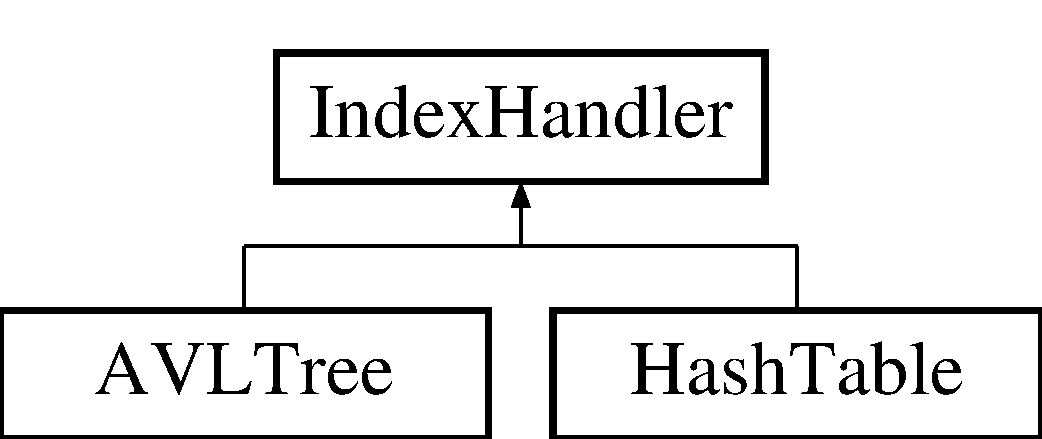
\includegraphics[height=2.000000cm]{class_index_handler}
\end{center}
\end{figure}
\subsection*{Public Member Functions}
\begin{DoxyCompactItemize}
\item 
\hyperlink{class_index_handler_a27748387661142a2eb545be6f0499996}{Index\+Handler} ()
\item 
virtual \hyperlink{class_index_handler_ad787ca8cf83345ecfe332d2c3b8f8009}{$\sim$\+Index\+Handler} ()
\item 
virtual std\+::string \hyperlink{class_index_handler_aaeb0f250516fbc93936efec2c3f21359}{get\+Class\+Type} ()=0
\item 
void \hyperlink{class_index_handler_aa916a3613990ed790d281863d685cfc5}{add\+Page} (\hyperlink{class_page}{Page} $\ast$)
\item 
virtual void \hyperlink{class_index_handler_a102638a9813e71541092a6695bd24012}{add\+To\+Index} (\hyperlink{class_page}{Page} $\ast$\&, std\+::string \&)=0
\item 
virtual set$<$ \hyperlink{class_page}{Page} $\ast$ $>$ \hyperlink{class_index_handler_ac3213de7636a1332440c3204957f4658}{search\+Index} (std\+::string)=0
\item 
virtual void \hyperlink{class_index_handler_a036ccca02cb734711a1e6a50b09a2b1f}{print\+Table} ()=0
\end{DoxyCompactItemize}


\subsection{Constructor \& Destructor Documentation}
\hypertarget{class_index_handler_a27748387661142a2eb545be6f0499996}{}\index{Index\+Handler@{Index\+Handler}!Index\+Handler@{Index\+Handler}}
\index{Index\+Handler@{Index\+Handler}!Index\+Handler@{Index\+Handler}}
\subsubsection[{Index\+Handler}]{\setlength{\rightskip}{0pt plus 5cm}Index\+Handler\+::\+Index\+Handler (
\begin{DoxyParamCaption}
{}
\end{DoxyParamCaption}
)}\label{class_index_handler_a27748387661142a2eb545be6f0499996}
\hypertarget{class_index_handler_ad787ca8cf83345ecfe332d2c3b8f8009}{}\index{Index\+Handler@{Index\+Handler}!````~Index\+Handler@{$\sim$\+Index\+Handler}}
\index{````~Index\+Handler@{$\sim$\+Index\+Handler}!Index\+Handler@{Index\+Handler}}
\subsubsection[{$\sim$\+Index\+Handler}]{\setlength{\rightskip}{0pt plus 5cm}Index\+Handler\+::$\sim$\+Index\+Handler (
\begin{DoxyParamCaption}
{}
\end{DoxyParamCaption}
)\hspace{0.3cm}{\ttfamily [virtual]}}\label{class_index_handler_ad787ca8cf83345ecfe332d2c3b8f8009}


\subsection{Member Function Documentation}
\hypertarget{class_index_handler_aa916a3613990ed790d281863d685cfc5}{}\index{Index\+Handler@{Index\+Handler}!add\+Page@{add\+Page}}
\index{add\+Page@{add\+Page}!Index\+Handler@{Index\+Handler}}
\subsubsection[{add\+Page}]{\setlength{\rightskip}{0pt plus 5cm}void Index\+Handler\+::add\+Page (
\begin{DoxyParamCaption}
\item[{{\bf Page} $\ast$}]{next\+Page}
\end{DoxyParamCaption}
)}\label{class_index_handler_aa916a3613990ed790d281863d685cfc5}
\hypertarget{class_index_handler_a102638a9813e71541092a6695bd24012}{}\index{Index\+Handler@{Index\+Handler}!add\+To\+Index@{add\+To\+Index}}
\index{add\+To\+Index@{add\+To\+Index}!Index\+Handler@{Index\+Handler}}
\subsubsection[{add\+To\+Index}]{\setlength{\rightskip}{0pt plus 5cm}virtual void Index\+Handler\+::add\+To\+Index (
\begin{DoxyParamCaption}
\item[{{\bf Page} $\ast$\&}]{, }
\item[{std\+::string \&}]{}
\end{DoxyParamCaption}
)\hspace{0.3cm}{\ttfamily [pure virtual]}}\label{class_index_handler_a102638a9813e71541092a6695bd24012}


Implemented in \hyperlink{class_hash_table_a9bee171516cca4930348a89fd0695b08}{Hash\+Table}.

\hypertarget{class_index_handler_aaeb0f250516fbc93936efec2c3f21359}{}\index{Index\+Handler@{Index\+Handler}!get\+Class\+Type@{get\+Class\+Type}}
\index{get\+Class\+Type@{get\+Class\+Type}!Index\+Handler@{Index\+Handler}}
\subsubsection[{get\+Class\+Type}]{\setlength{\rightskip}{0pt plus 5cm}virtual std\+::string Index\+Handler\+::get\+Class\+Type (
\begin{DoxyParamCaption}
{}
\end{DoxyParamCaption}
)\hspace{0.3cm}{\ttfamily [pure virtual]}}\label{class_index_handler_aaeb0f250516fbc93936efec2c3f21359}


Implemented in \hyperlink{class_a_v_l_tree_a708b6398ea1771de3077ca39c4005cca}{A\+V\+L\+Tree}, and \hyperlink{class_hash_table_ab5a5fca28242a0733cb95e0729d94761}{Hash\+Table}.

\hypertarget{class_index_handler_a036ccca02cb734711a1e6a50b09a2b1f}{}\index{Index\+Handler@{Index\+Handler}!print\+Table@{print\+Table}}
\index{print\+Table@{print\+Table}!Index\+Handler@{Index\+Handler}}
\subsubsection[{print\+Table}]{\setlength{\rightskip}{0pt plus 5cm}virtual void Index\+Handler\+::print\+Table (
\begin{DoxyParamCaption}
{}
\end{DoxyParamCaption}
)\hspace{0.3cm}{\ttfamily [pure virtual]}}\label{class_index_handler_a036ccca02cb734711a1e6a50b09a2b1f}


Implemented in \hyperlink{class_a_v_l_tree_aaeb00045be61c381863d43526b4dffe1}{A\+V\+L\+Tree}, and \hyperlink{class_hash_table_ab50be186df67a5621694cb2f692de3fa}{Hash\+Table}.

\hypertarget{class_index_handler_ac3213de7636a1332440c3204957f4658}{}\index{Index\+Handler@{Index\+Handler}!search\+Index@{search\+Index}}
\index{search\+Index@{search\+Index}!Index\+Handler@{Index\+Handler}}
\subsubsection[{search\+Index}]{\setlength{\rightskip}{0pt plus 5cm}virtual set$<${\bf Page}$\ast$$>$ Index\+Handler\+::search\+Index (
\begin{DoxyParamCaption}
\item[{std\+::string}]{}
\end{DoxyParamCaption}
)\hspace{0.3cm}{\ttfamily [pure virtual]}}\label{class_index_handler_ac3213de7636a1332440c3204957f4658}


Implemented in \hyperlink{class_hash_table_a3e63955ddf861d2feb8e6db908c19ac9}{Hash\+Table}.



The documentation for this class was generated from the following files\+:\begin{DoxyCompactItemize}
\item 
\hyperlink{_index_handler_8h}{Index\+Handler.\+h}\item 
\hyperlink{_index_handler_8cpp}{Index\+Handler.\+cpp}\end{DoxyCompactItemize}

\hypertarget{classstring__util_1_1less__string__compare}{\section{string\+\_\+util\+:\+:less\+\_\+string\+\_\+compare$<$ T $>$ Class Template Reference}
\label{classstring__util_1_1less__string__compare}\index{string\+\_\+util\+::less\+\_\+string\+\_\+compare$<$ T $>$@{string\+\_\+util\+::less\+\_\+string\+\_\+compare$<$ T $>$}}
}
Inheritance diagram for string\+\_\+util\+:\+:less\+\_\+string\+\_\+compare$<$ T $>$\+:\begin{figure}[H]
\begin{center}
\leavevmode
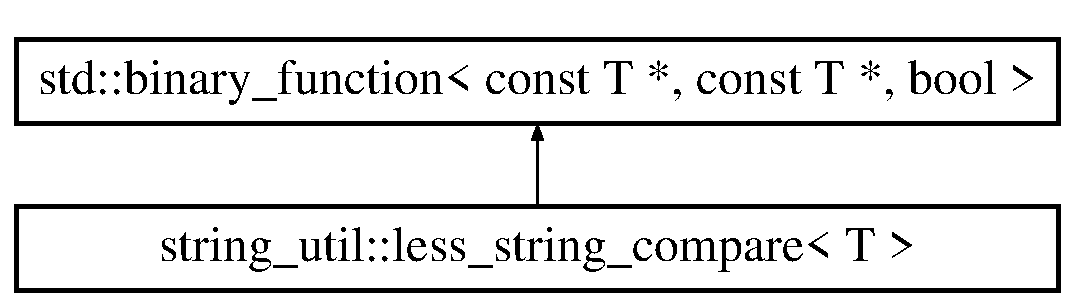
\includegraphics[height=2.000000cm]{classstring__util_1_1less__string__compare}
\end{center}
\end{figure}
\subsection*{Public Member Functions}
\begin{DoxyCompactItemize}
\item 
\hypertarget{classstring__util_1_1less__string__compare_aa97df82edd8f7e33e5715acf71759337}{bool {\bfseries operator()} (const T $\ast$a\+\_\+, const T $\ast$b\+\_\+) const }\label{classstring__util_1_1less__string__compare_aa97df82edd8f7e33e5715acf71759337}

\end{DoxyCompactItemize}


The documentation for this class was generated from the following file\+:\begin{DoxyCompactItemize}
\item 
string\+\_\+util.\+h\end{DoxyCompactItemize}

\hypertarget{classstring__util_1_1less__string__i__compare}{\section{string\+\_\+util\+:\+:less\+\_\+string\+\_\+i\+\_\+compare$<$ T $>$ Class Template Reference}
\label{classstring__util_1_1less__string__i__compare}\index{string\+\_\+util\+::less\+\_\+string\+\_\+i\+\_\+compare$<$ T $>$@{string\+\_\+util\+::less\+\_\+string\+\_\+i\+\_\+compare$<$ T $>$}}
}
Inheritance diagram for string\+\_\+util\+:\+:less\+\_\+string\+\_\+i\+\_\+compare$<$ T $>$\+:\begin{figure}[H]
\begin{center}
\leavevmode
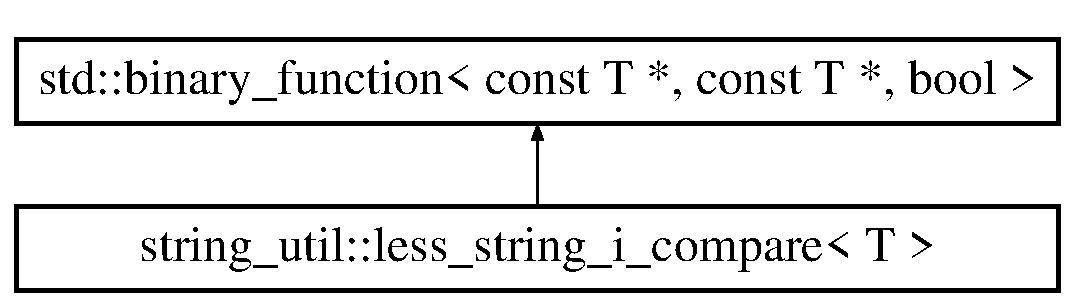
\includegraphics[height=2.000000cm]{classstring__util_1_1less__string__i__compare}
\end{center}
\end{figure}
\subsection*{Public Member Functions}
\begin{DoxyCompactItemize}
\item 
\hypertarget{classstring__util_1_1less__string__i__compare_ae2dd6a625b07bc51060805b30e7547a1}{bool {\bfseries operator()} (const T $\ast$a\+\_\+, const T $\ast$b\+\_\+) const }\label{classstring__util_1_1less__string__i__compare_ae2dd6a625b07bc51060805b30e7547a1}

\end{DoxyCompactItemize}


The documentation for this class was generated from the following file\+:\begin{DoxyCompactItemize}
\item 
string\+\_\+util.\+h\end{DoxyCompactItemize}

\hypertarget{classstring__util_1_1less__string__n__compare}{\section{string\+\_\+util\+:\+:less\+\_\+string\+\_\+n\+\_\+compare$<$ T $>$ Class Template Reference}
\label{classstring__util_1_1less__string__n__compare}\index{string\+\_\+util\+::less\+\_\+string\+\_\+n\+\_\+compare$<$ T $>$@{string\+\_\+util\+::less\+\_\+string\+\_\+n\+\_\+compare$<$ T $>$}}
}
Inheritance diagram for string\+\_\+util\+:\+:less\+\_\+string\+\_\+n\+\_\+compare$<$ T $>$\+:\begin{figure}[H]
\begin{center}
\leavevmode
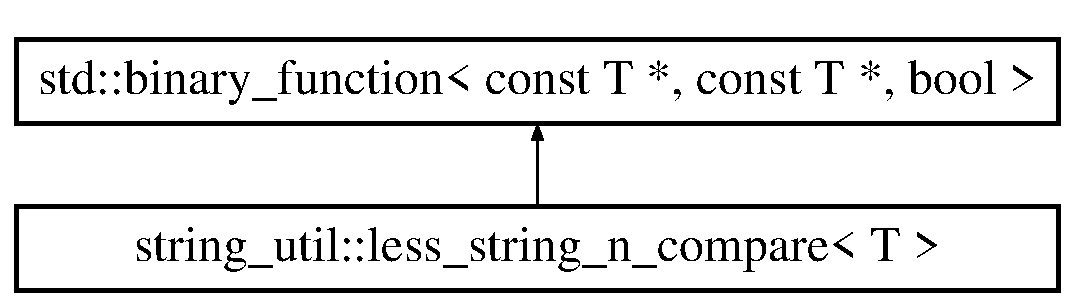
\includegraphics[height=2.000000cm]{classstring__util_1_1less__string__n__compare}
\end{center}
\end{figure}
\subsection*{Public Member Functions}
\begin{DoxyCompactItemize}
\item 
\hypertarget{classstring__util_1_1less__string__n__compare_a42b269c0aa27c5ace8b3eeb782f6d335}{{\bfseries less\+\_\+string\+\_\+n\+\_\+compare} (size\+\_\+t comparison\+\_\+size)}\label{classstring__util_1_1less__string__n__compare_a42b269c0aa27c5ace8b3eeb782f6d335}

\item 
\hypertarget{classstring__util_1_1less__string__n__compare_ab6f6bb1fbd6421cb848bba88ce18f6e0}{bool {\bfseries operator()} (const T $\ast$a\+\_\+, const T $\ast$b\+\_\+) const }\label{classstring__util_1_1less__string__n__compare_ab6f6bb1fbd6421cb848bba88ce18f6e0}

\end{DoxyCompactItemize}


The documentation for this class was generated from the following file\+:\begin{DoxyCompactItemize}
\item 
string\+\_\+util.\+h\end{DoxyCompactItemize}

\hypertarget{classstring__util_1_1less__string__natural__order__i__compare}{\section{string\+\_\+util\+:\+:less\+\_\+string\+\_\+natural\+\_\+order\+\_\+i\+\_\+compare$<$ T $>$ Class Template Reference}
\label{classstring__util_1_1less__string__natural__order__i__compare}\index{string\+\_\+util\+::less\+\_\+string\+\_\+natural\+\_\+order\+\_\+i\+\_\+compare$<$ T $>$@{string\+\_\+util\+::less\+\_\+string\+\_\+natural\+\_\+order\+\_\+i\+\_\+compare$<$ T $>$}}
}
Inheritance diagram for string\+\_\+util\+:\+:less\+\_\+string\+\_\+natural\+\_\+order\+\_\+i\+\_\+compare$<$ T $>$\+:\begin{figure}[H]
\begin{center}
\leavevmode
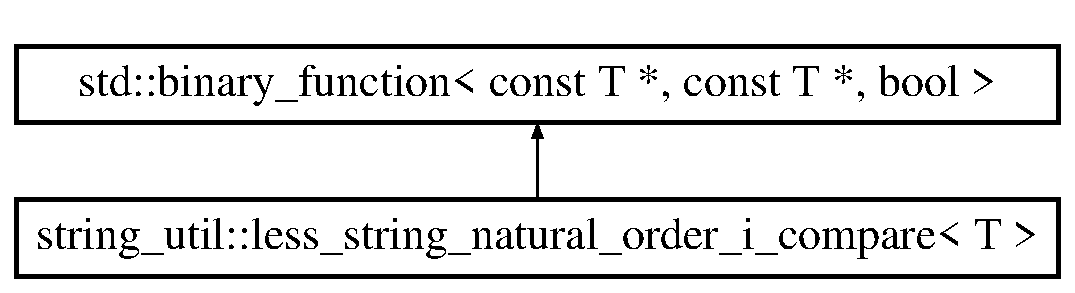
\includegraphics[height=2.000000cm]{classstring__util_1_1less__string__natural__order__i__compare}
\end{center}
\end{figure}
\subsection*{Public Member Functions}
\begin{DoxyCompactItemize}
\item 
\hypertarget{classstring__util_1_1less__string__natural__order__i__compare_a213ba84bcb81fa025951194acbdb899c}{bool {\bfseries operator()} (const T $\ast$a\+\_\+, const T $\ast$b\+\_\+) const }\label{classstring__util_1_1less__string__natural__order__i__compare_a213ba84bcb81fa025951194acbdb899c}

\end{DoxyCompactItemize}


The documentation for this class was generated from the following file\+:\begin{DoxyCompactItemize}
\item 
string\+\_\+util.\+h\end{DoxyCompactItemize}

\hypertarget{classstring__util_1_1less__string__ni__compare}{\section{string\+\_\+util\+:\+:less\+\_\+string\+\_\+ni\+\_\+compare$<$ T $>$ Class Template Reference}
\label{classstring__util_1_1less__string__ni__compare}\index{string\+\_\+util\+::less\+\_\+string\+\_\+ni\+\_\+compare$<$ T $>$@{string\+\_\+util\+::less\+\_\+string\+\_\+ni\+\_\+compare$<$ T $>$}}
}
Inheritance diagram for string\+\_\+util\+:\+:less\+\_\+string\+\_\+ni\+\_\+compare$<$ T $>$\+:\begin{figure}[H]
\begin{center}
\leavevmode
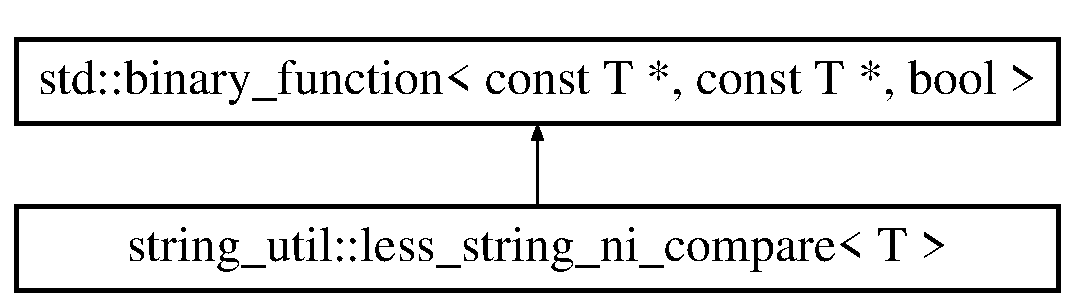
\includegraphics[height=2.000000cm]{classstring__util_1_1less__string__ni__compare}
\end{center}
\end{figure}
\subsection*{Public Member Functions}
\begin{DoxyCompactItemize}
\item 
\hypertarget{classstring__util_1_1less__string__ni__compare_aec49bc79089ab2e54ff4752bbbabe6bf}{{\bfseries less\+\_\+string\+\_\+ni\+\_\+compare} (size\+\_\+t comparison\+\_\+size)}\label{classstring__util_1_1less__string__ni__compare_aec49bc79089ab2e54ff4752bbbabe6bf}

\item 
\hypertarget{classstring__util_1_1less__string__ni__compare_a6050f7d7b4998343cc5c46dca8b28bcc}{bool {\bfseries operator()} (const T $\ast$a\+\_\+, const T $\ast$b\+\_\+) const }\label{classstring__util_1_1less__string__ni__compare_a6050f7d7b4998343cc5c46dca8b28bcc}

\end{DoxyCompactItemize}


The documentation for this class was generated from the following file\+:\begin{DoxyCompactItemize}
\item 
string\+\_\+util.\+h\end{DoxyCompactItemize}

\hypertarget{classstemming_1_1no__op__stem}{\section{stemming\+:\+:no\+\_\+op\+\_\+stem$<$ string\+\_\+type\+T $>$ Class Template Reference}
\label{classstemming_1_1no__op__stem}\index{stemming\+::no\+\_\+op\+\_\+stem$<$ string\+\_\+type\+T $>$@{stemming\+::no\+\_\+op\+\_\+stem$<$ string\+\_\+type\+T $>$}}
}
\subsection*{Public Member Functions}
\begin{DoxyCompactItemize}
\item 
\hypertarget{classstemming_1_1no__op__stem_ada7ad3e0b3a7559f4c8907bf25bbd14c}{void \hyperlink{classstemming_1_1no__op__stem_ada7ad3e0b3a7559f4c8907bf25bbd14c}{operator()} (const string\+\_\+type\+T \&text) const }\label{classstemming_1_1no__op__stem_ada7ad3e0b3a7559f4c8907bf25bbd14c}

\begin{DoxyCompactList}\small\item\em No-\/op stemming of declared string type. \end{DoxyCompactList}\item 
\hypertarget{classstemming_1_1no__op__stem_a7ef5607b060c99e699455ea4c1d0038a}{{\footnotesize template$<$typename T $>$ }\\void \hyperlink{classstemming_1_1no__op__stem_a7ef5607b060c99e699455ea4c1d0038a}{operator()} (const T \&text) const }\label{classstemming_1_1no__op__stem_a7ef5607b060c99e699455ea4c1d0038a}

\begin{DoxyCompactList}\small\item\em No-\/op stemming of flexible string type. \end{DoxyCompactList}\end{DoxyCompactItemize}


The documentation for this class was generated from the following file\+:\begin{DoxyCompactItemize}
\item 
stemming.\+h\end{DoxyCompactItemize}

\hypertarget{class_node}{\section{Node Class Reference}
\label{class_node}\index{Node@{Node}}
}
Inheritance diagram for Node\+:\begin{figure}[H]
\begin{center}
\leavevmode
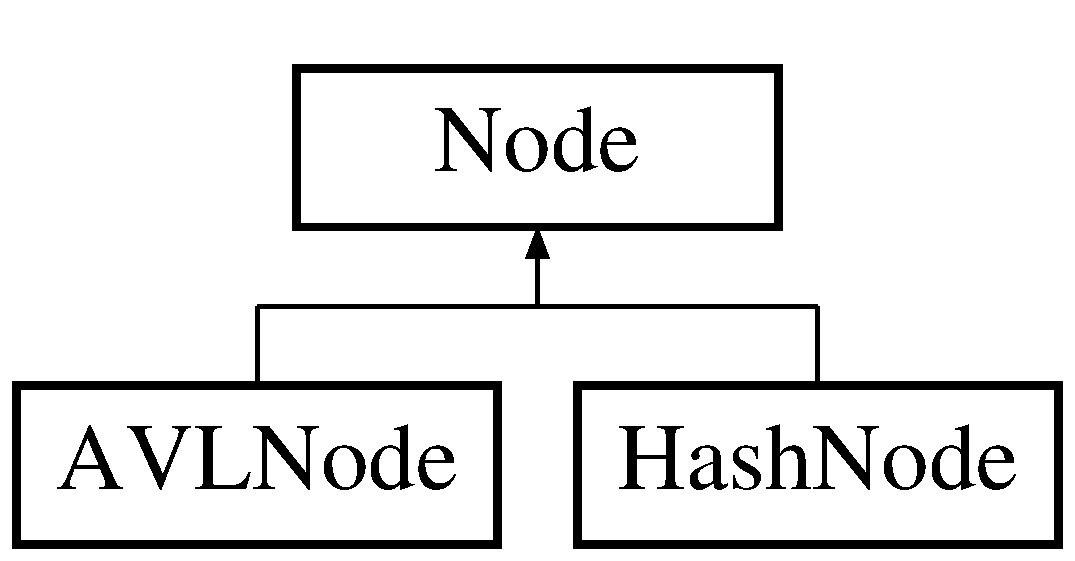
\includegraphics[height=2.000000cm]{class_node}
\end{center}
\end{figure}
\subsection*{Public Member Functions}
\begin{DoxyCompactItemize}
\item 
\hypertarget{class_node_a521cc0c4ebb153869947b76df9e0eada}{{\bfseries Node} (\hyperlink{class_page}{Page} $\ast$, string)}\label{class_node_a521cc0c4ebb153869947b76df9e0eada}

\item 
\hypertarget{class_node_ac5298373555f67634e27e5c739e7c94b}{string {\bfseries get\+Name} ()}\label{class_node_ac5298373555f67634e27e5c739e7c94b}

\item 
\hypertarget{class_node_a1fa90b3fa1a6ad3bbe616c4a6c0ba831}{set$<$ \hyperlink{class_page}{Page} $\ast$ $>$ {\bfseries get\+Set\+Of\+Pages} ()}\label{class_node_a1fa90b3fa1a6ad3bbe616c4a6c0ba831}

\item 
\hypertarget{class_node_ac6ab8994f203f84c076602540f003f7c}{void {\bfseries set\+Word} (string)}\label{class_node_ac6ab8994f203f84c076602540f003f7c}

\item 
\hypertarget{class_node_a742fe1af9dc4e51b0153a430bf2761bf}{set$<$ \hyperlink{class_page}{Page} $\ast$ $>$ {\bfseries get\+Binder} ()}\label{class_node_a742fe1af9dc4e51b0153a430bf2761bf}

\item 
\hypertarget{class_node_a921c6be0a1bb9c49ecaecaf675cd7260}{string {\bfseries get\+Word} ()}\label{class_node_a921c6be0a1bb9c49ecaecaf675cd7260}

\item 
\hypertarget{class_node_a2e469c97259b2823f9d9611da3ae2184}{void {\bfseries add\+To\+Binder} (\hyperlink{class_page}{Page} $\ast$\&)}\label{class_node_a2e469c97259b2823f9d9611da3ae2184}

\end{DoxyCompactItemize}


The documentation for this class was generated from the following files\+:\begin{DoxyCompactItemize}
\item 
Node.\+h\item 
Node.\+cpp\end{DoxyCompactItemize}

\hypertarget{class_page}{}\section{Page Class Reference}
\label{class_page}\index{Page@{Page}}


{\ttfamily \#include $<$Page.\+h$>$}

\subsection*{Public Member Functions}
\begin{DoxyCompactItemize}
\item 
\hyperlink{class_page_a9a7cc22d5459498ce638c54ae966c79b}{Page} ()
\item 
void \hyperlink{class_page_acf477f6eb17bab9955041f62cf773e8d}{set\+Title} (string)
\item 
void \hyperlink{class_page_ac482ec0d499e8c4d61f65bec3c845e05}{set\+Id} (unsigned long)
\item 
void \hyperlink{class_page_aa035203c86eb29a7121987ef5bfa1faf}{set\+Contributing\+User} (string)
\item 
void \hyperlink{class_page_a12df427d5f2620b2e912590eb1c81d32}{set\+Date} (string)
\item 
void \hyperlink{class_page_ada78e7ad8b4111afa5dd503151946e70}{set\+Frequency} (int, int)
\item 
void \hyperlink{class_page_a3f82c5cc09e31dc064246984ce7b7c17}{set\+Full\+Text} (string)
\item 
string \hyperlink{class_page_ad9647bb36d7587217dae9039aaf9d0db}{get\+Full\+Text} ()
\item 
string \hyperlink{class_page_ad8984dc2ec1c9d62343e35724080ee46}{get\+Title} ()
\item 
unsigned long \hyperlink{class_page_a8ce274bdff4b0f02131b0142dfd38dde}{get\+Id} ()
\item 
string \hyperlink{class_page_aa21e1e663df6f64d0670f4f9ac97330c}{get\+Contributing\+User} ()
\item 
string \hyperlink{class_page_aa9f674aaecb16f3ef02d54d0e42abe49}{get\+Date} ()
\item 
vector$<$ string $>$ \hyperlink{class_page_a31af27b5aa8f44f6bfb95fdbf555477c}{get\+Keywords} ()
\item 
int \hyperlink{class_page_a34588144ffb1c839e179f43aa7d9977c}{get\+Frequency} (int)
\item 
string \hyperlink{class_page_a0b43e8cd80b96011df19d083e6436a0f}{get\+Keyword\+At\+Index} (int)
\item 
void \hyperlink{class_page_a5650ea40b701dd7e15c7aa90fc819358}{increment\+Freq} (int)
\item 
int \hyperlink{class_page_a16d01583e3275c3a3c30793408f9865f}{add\+Keyword} (string \&)
\item 
\hyperlink{class_page_a2341fff1cc032ab6528874175e7dd841}{$\sim$\+Page} ()
\end{DoxyCompactItemize}
\subsection*{Static Public Member Functions}
\begin{DoxyCompactItemize}
\item 
static int \hyperlink{class_page_a8f1ef6fe4e22e67941a00bb6f5ff4be4}{binary\+Search} (vector$<$ string $>$ \&, string, int, int)
\end{DoxyCompactItemize}
\subsection*{Public Attributes}
\begin{DoxyCompactItemize}
\item 
string \hyperlink{class_page_a8713192624b3bc969533e4ebd39516c3}{full\+Text}
\end{DoxyCompactItemize}


\subsection{Constructor \& Destructor Documentation}
\hypertarget{class_page_a9a7cc22d5459498ce638c54ae966c79b}{}\index{Page@{Page}!Page@{Page}}
\index{Page@{Page}!Page@{Page}}
\subsubsection[{Page}]{\setlength{\rightskip}{0pt plus 5cm}Page\+::\+Page (
\begin{DoxyParamCaption}
{}
\end{DoxyParamCaption}
)}\label{class_page_a9a7cc22d5459498ce638c54ae966c79b}
\hypertarget{class_page_a2341fff1cc032ab6528874175e7dd841}{}\index{Page@{Page}!````~Page@{$\sim$\+Page}}
\index{````~Page@{$\sim$\+Page}!Page@{Page}}
\subsubsection[{$\sim$\+Page}]{\setlength{\rightskip}{0pt plus 5cm}Page\+::$\sim$\+Page (
\begin{DoxyParamCaption}
{}
\end{DoxyParamCaption}
)}\label{class_page_a2341fff1cc032ab6528874175e7dd841}


\subsection{Member Function Documentation}
\hypertarget{class_page_a16d01583e3275c3a3c30793408f9865f}{}\index{Page@{Page}!add\+Keyword@{add\+Keyword}}
\index{add\+Keyword@{add\+Keyword}!Page@{Page}}
\subsubsection[{add\+Keyword}]{\setlength{\rightskip}{0pt plus 5cm}int Page\+::add\+Keyword (
\begin{DoxyParamCaption}
\item[{string \&}]{keyword}
\end{DoxyParamCaption}
)}\label{class_page_a16d01583e3275c3a3c30793408f9865f}
\hypertarget{class_page_a8f1ef6fe4e22e67941a00bb6f5ff4be4}{}\index{Page@{Page}!binary\+Search@{binary\+Search}}
\index{binary\+Search@{binary\+Search}!Page@{Page}}
\subsubsection[{binary\+Search}]{\setlength{\rightskip}{0pt plus 5cm}int Page\+::binary\+Search (
\begin{DoxyParamCaption}
\item[{vector$<$ string $>$ \&}]{vc, }
\item[{string}]{kw, }
\item[{int}]{low, }
\item[{int}]{high}
\end{DoxyParamCaption}
)\hspace{0.3cm}{\ttfamily [static]}}\label{class_page_a8f1ef6fe4e22e67941a00bb6f5ff4be4}
\hypertarget{class_page_aa21e1e663df6f64d0670f4f9ac97330c}{}\index{Page@{Page}!get\+Contributing\+User@{get\+Contributing\+User}}
\index{get\+Contributing\+User@{get\+Contributing\+User}!Page@{Page}}
\subsubsection[{get\+Contributing\+User}]{\setlength{\rightskip}{0pt plus 5cm}string Page\+::get\+Contributing\+User (
\begin{DoxyParamCaption}
{}
\end{DoxyParamCaption}
)}\label{class_page_aa21e1e663df6f64d0670f4f9ac97330c}
\hypertarget{class_page_aa9f674aaecb16f3ef02d54d0e42abe49}{}\index{Page@{Page}!get\+Date@{get\+Date}}
\index{get\+Date@{get\+Date}!Page@{Page}}
\subsubsection[{get\+Date}]{\setlength{\rightskip}{0pt plus 5cm}string Page\+::get\+Date (
\begin{DoxyParamCaption}
{}
\end{DoxyParamCaption}
)}\label{class_page_aa9f674aaecb16f3ef02d54d0e42abe49}
\hypertarget{class_page_a34588144ffb1c839e179f43aa7d9977c}{}\index{Page@{Page}!get\+Frequency@{get\+Frequency}}
\index{get\+Frequency@{get\+Frequency}!Page@{Page}}
\subsubsection[{get\+Frequency}]{\setlength{\rightskip}{0pt plus 5cm}int Page\+::get\+Frequency (
\begin{DoxyParamCaption}
\item[{int}]{index}
\end{DoxyParamCaption}
)}\label{class_page_a34588144ffb1c839e179f43aa7d9977c}
\hypertarget{class_page_ad9647bb36d7587217dae9039aaf9d0db}{}\index{Page@{Page}!get\+Full\+Text@{get\+Full\+Text}}
\index{get\+Full\+Text@{get\+Full\+Text}!Page@{Page}}
\subsubsection[{get\+Full\+Text}]{\setlength{\rightskip}{0pt plus 5cm}string Page\+::get\+Full\+Text (
\begin{DoxyParamCaption}
{}
\end{DoxyParamCaption}
)}\label{class_page_ad9647bb36d7587217dae9039aaf9d0db}
\hypertarget{class_page_a8ce274bdff4b0f02131b0142dfd38dde}{}\index{Page@{Page}!get\+Id@{get\+Id}}
\index{get\+Id@{get\+Id}!Page@{Page}}
\subsubsection[{get\+Id}]{\setlength{\rightskip}{0pt plus 5cm}unsigned long Page\+::get\+Id (
\begin{DoxyParamCaption}
{}
\end{DoxyParamCaption}
)}\label{class_page_a8ce274bdff4b0f02131b0142dfd38dde}
\hypertarget{class_page_a0b43e8cd80b96011df19d083e6436a0f}{}\index{Page@{Page}!get\+Keyword\+At\+Index@{get\+Keyword\+At\+Index}}
\index{get\+Keyword\+At\+Index@{get\+Keyword\+At\+Index}!Page@{Page}}
\subsubsection[{get\+Keyword\+At\+Index}]{\setlength{\rightskip}{0pt plus 5cm}string Page\+::get\+Keyword\+At\+Index (
\begin{DoxyParamCaption}
\item[{int}]{index}
\end{DoxyParamCaption}
)}\label{class_page_a0b43e8cd80b96011df19d083e6436a0f}
\hypertarget{class_page_a31af27b5aa8f44f6bfb95fdbf555477c}{}\index{Page@{Page}!get\+Keywords@{get\+Keywords}}
\index{get\+Keywords@{get\+Keywords}!Page@{Page}}
\subsubsection[{get\+Keywords}]{\setlength{\rightskip}{0pt plus 5cm}vector$<$ string $>$ Page\+::get\+Keywords (
\begin{DoxyParamCaption}
{}
\end{DoxyParamCaption}
)}\label{class_page_a31af27b5aa8f44f6bfb95fdbf555477c}
\hypertarget{class_page_ad8984dc2ec1c9d62343e35724080ee46}{}\index{Page@{Page}!get\+Title@{get\+Title}}
\index{get\+Title@{get\+Title}!Page@{Page}}
\subsubsection[{get\+Title}]{\setlength{\rightskip}{0pt plus 5cm}string Page\+::get\+Title (
\begin{DoxyParamCaption}
{}
\end{DoxyParamCaption}
)}\label{class_page_ad8984dc2ec1c9d62343e35724080ee46}
\hypertarget{class_page_a5650ea40b701dd7e15c7aa90fc819358}{}\index{Page@{Page}!increment\+Freq@{increment\+Freq}}
\index{increment\+Freq@{increment\+Freq}!Page@{Page}}
\subsubsection[{increment\+Freq}]{\setlength{\rightskip}{0pt plus 5cm}void Page\+::increment\+Freq (
\begin{DoxyParamCaption}
\item[{int}]{index}
\end{DoxyParamCaption}
)}\label{class_page_a5650ea40b701dd7e15c7aa90fc819358}
\hypertarget{class_page_aa035203c86eb29a7121987ef5bfa1faf}{}\index{Page@{Page}!set\+Contributing\+User@{set\+Contributing\+User}}
\index{set\+Contributing\+User@{set\+Contributing\+User}!Page@{Page}}
\subsubsection[{set\+Contributing\+User}]{\setlength{\rightskip}{0pt plus 5cm}void Page\+::set\+Contributing\+User (
\begin{DoxyParamCaption}
\item[{string}]{username}
\end{DoxyParamCaption}
)}\label{class_page_aa035203c86eb29a7121987ef5bfa1faf}
\hypertarget{class_page_a12df427d5f2620b2e912590eb1c81d32}{}\index{Page@{Page}!set\+Date@{set\+Date}}
\index{set\+Date@{set\+Date}!Page@{Page}}
\subsubsection[{set\+Date}]{\setlength{\rightskip}{0pt plus 5cm}void Page\+::set\+Date (
\begin{DoxyParamCaption}
\item[{string}]{d}
\end{DoxyParamCaption}
)}\label{class_page_a12df427d5f2620b2e912590eb1c81d32}
\hypertarget{class_page_ada78e7ad8b4111afa5dd503151946e70}{}\index{Page@{Page}!set\+Frequency@{set\+Frequency}}
\index{set\+Frequency@{set\+Frequency}!Page@{Page}}
\subsubsection[{set\+Frequency}]{\setlength{\rightskip}{0pt plus 5cm}void Page\+::set\+Frequency (
\begin{DoxyParamCaption}
\item[{int}]{index, }
\item[{int}]{freq}
\end{DoxyParamCaption}
)}\label{class_page_ada78e7ad8b4111afa5dd503151946e70}
\hypertarget{class_page_a3f82c5cc09e31dc064246984ce7b7c17}{}\index{Page@{Page}!set\+Full\+Text@{set\+Full\+Text}}
\index{set\+Full\+Text@{set\+Full\+Text}!Page@{Page}}
\subsubsection[{set\+Full\+Text}]{\setlength{\rightskip}{0pt plus 5cm}void Page\+::set\+Full\+Text (
\begin{DoxyParamCaption}
\item[{string}]{text}
\end{DoxyParamCaption}
)}\label{class_page_a3f82c5cc09e31dc064246984ce7b7c17}
\hypertarget{class_page_ac482ec0d499e8c4d61f65bec3c845e05}{}\index{Page@{Page}!set\+Id@{set\+Id}}
\index{set\+Id@{set\+Id}!Page@{Page}}
\subsubsection[{set\+Id}]{\setlength{\rightskip}{0pt plus 5cm}void Page\+::set\+Id (
\begin{DoxyParamCaption}
\item[{unsigned long}]{num}
\end{DoxyParamCaption}
)}\label{class_page_ac482ec0d499e8c4d61f65bec3c845e05}
\hypertarget{class_page_acf477f6eb17bab9955041f62cf773e8d}{}\index{Page@{Page}!set\+Title@{set\+Title}}
\index{set\+Title@{set\+Title}!Page@{Page}}
\subsubsection[{set\+Title}]{\setlength{\rightskip}{0pt plus 5cm}void Page\+::set\+Title (
\begin{DoxyParamCaption}
\item[{string}]{t}
\end{DoxyParamCaption}
)}\label{class_page_acf477f6eb17bab9955041f62cf773e8d}


\subsection{Member Data Documentation}
\hypertarget{class_page_a8713192624b3bc969533e4ebd39516c3}{}\index{Page@{Page}!full\+Text@{full\+Text}}
\index{full\+Text@{full\+Text}!Page@{Page}}
\subsubsection[{full\+Text}]{\setlength{\rightskip}{0pt plus 5cm}string Page\+::full\+Text}\label{class_page_a8713192624b3bc969533e4ebd39516c3}


The documentation for this class was generated from the following files\+:\begin{DoxyCompactItemize}
\item 
\hyperlink{_page_8h}{Page.\+h}\item 
\hyperlink{_page_8cpp}{Page.\+cpp}\end{DoxyCompactItemize}

\hypertarget{class_query}{}\section{Query Class Reference}
\label{class_query}\index{Query@{Query}}


{\ttfamily \#include $<$Query.\+h$>$}

\subsection*{Public Member Functions}
\begin{DoxyCompactItemize}
\item 
\hyperlink{class_query_a4c1633236bdb9fa8d3fd3572a469889d}{Query} ()
\item 
std\+::vector$<$ std\+::string $>$ \hyperlink{class_query_a509091fc6e1bba8544991403a6d7b4b7}{getand\+Args} ()
\item 
std\+::vector$<$ std\+::string $>$ \hyperlink{class_query_ab90fc81524045a085b472dad8e6032bd}{getor\+Args} ()
\item 
std\+::vector$<$ std\+::string $>$ \hyperlink{class_query_a83014fdd314c75564ef1746fccd77407}{getnot\+Args} ()
\item 
std\+::vector$<$ std\+::string $>$ \hyperlink{class_query_afed0bd695e2b355d42ae78a79c2b2592}{getnorm\+Args} ()
\item 
std\+::string \hyperlink{class_query_aa2e86853eac7f292d4894cf8ef4260b0}{getand\+Args} (int)
\item 
std\+::string \hyperlink{class_query_ae3966de9b3bdba292a67b0e418a9d146}{getor\+Args} (int)
\item 
std\+::string \hyperlink{class_query_a7ef802901ce6e3b7b68e46b2f6659b18}{getnot\+Args} (int)
\item 
std\+::string \hyperlink{class_query_aa7d5b960f0d1cd7c83b7d191ac371d0a}{getnorm\+Args} (int)
\item 
void \hyperlink{class_query_a0497175553ef811642c5b2b3c0bd1ca2}{setand\+Args} (int, std\+::string)
\item 
void \hyperlink{class_query_afb2f5f87786fc282fefface523a81138}{setor\+Args} (int, std\+::string)
\item 
void \hyperlink{class_query_aef14c309f6f5880066f649a8f47fe3bc}{setnot\+Args} (int, std\+::string)
\item 
void \hyperlink{class_query_a24a65f32cdc1c1ee4246cbf480763557}{setnorm\+Args} (int, std\+::string)
\item 
void \hyperlink{class_query_a308104a6371bdf950435593413d527a6}{addand\+Args} (std\+::string)
\item 
void \hyperlink{class_query_aa19cc7a02d5e11c44118760bad4d0f50}{addor\+Args} (std\+::string)
\item 
void \hyperlink{class_query_a1923e0fdb1a976e23dc79731722d4fa3}{addnot\+Args} (std\+::string)
\item 
void \hyperlink{class_query_a038cf2204b03b09bd8423ee919c6866b}{addnorm\+Args} (std\+::string)
\item 
void \hyperlink{class_query_aa8b2a46725fdad4e06aad405b6c18227}{clear\+Query} ()
\item 
\hyperlink{class_query_aad0c964335e9809cc7e22af34e9e8410}{$\sim$\+Query} ()
\end{DoxyCompactItemize}


\subsection{Detailed Description}
\hyperlink{class_query}{Query} header file holds each keyword needing to be searched in query Sam Hunter and Morgan Monzingo 

\subsection{Constructor \& Destructor Documentation}
\hypertarget{class_query_a4c1633236bdb9fa8d3fd3572a469889d}{}\index{Query@{Query}!Query@{Query}}
\index{Query@{Query}!Query@{Query}}
\subsubsection[{Query}]{\setlength{\rightskip}{0pt plus 5cm}Query\+::\+Query (
\begin{DoxyParamCaption}
{}
\end{DoxyParamCaption}
)}\label{class_query_a4c1633236bdb9fa8d3fd3572a469889d}
\hypertarget{class_query_aad0c964335e9809cc7e22af34e9e8410}{}\index{Query@{Query}!````~Query@{$\sim$\+Query}}
\index{````~Query@{$\sim$\+Query}!Query@{Query}}
\subsubsection[{$\sim$\+Query}]{\setlength{\rightskip}{0pt plus 5cm}Query\+::$\sim$\+Query (
\begin{DoxyParamCaption}
{}
\end{DoxyParamCaption}
)}\label{class_query_aad0c964335e9809cc7e22af34e9e8410}


\subsection{Member Function Documentation}
\hypertarget{class_query_a308104a6371bdf950435593413d527a6}{}\index{Query@{Query}!addand\+Args@{addand\+Args}}
\index{addand\+Args@{addand\+Args}!Query@{Query}}
\subsubsection[{addand\+Args}]{\setlength{\rightskip}{0pt plus 5cm}void Query\+::addand\+Args (
\begin{DoxyParamCaption}
\item[{std\+::string}]{and\+Arg}
\end{DoxyParamCaption}
)}\label{class_query_a308104a6371bdf950435593413d527a6}
\hypertarget{class_query_a038cf2204b03b09bd8423ee919c6866b}{}\index{Query@{Query}!addnorm\+Args@{addnorm\+Args}}
\index{addnorm\+Args@{addnorm\+Args}!Query@{Query}}
\subsubsection[{addnorm\+Args}]{\setlength{\rightskip}{0pt plus 5cm}void Query\+::addnorm\+Args (
\begin{DoxyParamCaption}
\item[{std\+::string}]{norm\+Arg}
\end{DoxyParamCaption}
)}\label{class_query_a038cf2204b03b09bd8423ee919c6866b}
\hypertarget{class_query_a1923e0fdb1a976e23dc79731722d4fa3}{}\index{Query@{Query}!addnot\+Args@{addnot\+Args}}
\index{addnot\+Args@{addnot\+Args}!Query@{Query}}
\subsubsection[{addnot\+Args}]{\setlength{\rightskip}{0pt plus 5cm}void Query\+::addnot\+Args (
\begin{DoxyParamCaption}
\item[{std\+::string}]{}
\end{DoxyParamCaption}
)}\label{class_query_a1923e0fdb1a976e23dc79731722d4fa3}
\hypertarget{class_query_aa19cc7a02d5e11c44118760bad4d0f50}{}\index{Query@{Query}!addor\+Args@{addor\+Args}}
\index{addor\+Args@{addor\+Args}!Query@{Query}}
\subsubsection[{addor\+Args}]{\setlength{\rightskip}{0pt plus 5cm}void Query\+::addor\+Args (
\begin{DoxyParamCaption}
\item[{std\+::string}]{or\+Arg}
\end{DoxyParamCaption}
)}\label{class_query_aa19cc7a02d5e11c44118760bad4d0f50}
\hypertarget{class_query_aa8b2a46725fdad4e06aad405b6c18227}{}\index{Query@{Query}!clear\+Query@{clear\+Query}}
\index{clear\+Query@{clear\+Query}!Query@{Query}}
\subsubsection[{clear\+Query}]{\setlength{\rightskip}{0pt plus 5cm}void Query\+::clear\+Query (
\begin{DoxyParamCaption}
{}
\end{DoxyParamCaption}
)}\label{class_query_aa8b2a46725fdad4e06aad405b6c18227}
\hypertarget{class_query_a509091fc6e1bba8544991403a6d7b4b7}{}\index{Query@{Query}!getand\+Args@{getand\+Args}}
\index{getand\+Args@{getand\+Args}!Query@{Query}}
\subsubsection[{getand\+Args}]{\setlength{\rightskip}{0pt plus 5cm}std\+::vector$<$ std\+::string $>$ Query\+::getand\+Args (
\begin{DoxyParamCaption}
{}
\end{DoxyParamCaption}
)}\label{class_query_a509091fc6e1bba8544991403a6d7b4b7}
\hypertarget{class_query_aa2e86853eac7f292d4894cf8ef4260b0}{}\index{Query@{Query}!getand\+Args@{getand\+Args}}
\index{getand\+Args@{getand\+Args}!Query@{Query}}
\subsubsection[{getand\+Args}]{\setlength{\rightskip}{0pt plus 5cm}std\+::string Query\+::getand\+Args (
\begin{DoxyParamCaption}
\item[{int}]{index}
\end{DoxyParamCaption}
)}\label{class_query_aa2e86853eac7f292d4894cf8ef4260b0}
\hypertarget{class_query_afed0bd695e2b355d42ae78a79c2b2592}{}\index{Query@{Query}!getnorm\+Args@{getnorm\+Args}}
\index{getnorm\+Args@{getnorm\+Args}!Query@{Query}}
\subsubsection[{getnorm\+Args}]{\setlength{\rightskip}{0pt plus 5cm}std\+::vector$<$ std\+::string $>$ Query\+::getnorm\+Args (
\begin{DoxyParamCaption}
{}
\end{DoxyParamCaption}
)}\label{class_query_afed0bd695e2b355d42ae78a79c2b2592}
\hypertarget{class_query_aa7d5b960f0d1cd7c83b7d191ac371d0a}{}\index{Query@{Query}!getnorm\+Args@{getnorm\+Args}}
\index{getnorm\+Args@{getnorm\+Args}!Query@{Query}}
\subsubsection[{getnorm\+Args}]{\setlength{\rightskip}{0pt plus 5cm}std\+::string Query\+::getnorm\+Args (
\begin{DoxyParamCaption}
\item[{int}]{index}
\end{DoxyParamCaption}
)}\label{class_query_aa7d5b960f0d1cd7c83b7d191ac371d0a}
\hypertarget{class_query_a83014fdd314c75564ef1746fccd77407}{}\index{Query@{Query}!getnot\+Args@{getnot\+Args}}
\index{getnot\+Args@{getnot\+Args}!Query@{Query}}
\subsubsection[{getnot\+Args}]{\setlength{\rightskip}{0pt plus 5cm}std\+::vector$<$ std\+::string $>$ Query\+::getnot\+Args (
\begin{DoxyParamCaption}
{}
\end{DoxyParamCaption}
)}\label{class_query_a83014fdd314c75564ef1746fccd77407}
\hypertarget{class_query_a7ef802901ce6e3b7b68e46b2f6659b18}{}\index{Query@{Query}!getnot\+Args@{getnot\+Args}}
\index{getnot\+Args@{getnot\+Args}!Query@{Query}}
\subsubsection[{getnot\+Args}]{\setlength{\rightskip}{0pt plus 5cm}std\+::string Query\+::getnot\+Args (
\begin{DoxyParamCaption}
\item[{int}]{index}
\end{DoxyParamCaption}
)}\label{class_query_a7ef802901ce6e3b7b68e46b2f6659b18}
\hypertarget{class_query_ab90fc81524045a085b472dad8e6032bd}{}\index{Query@{Query}!getor\+Args@{getor\+Args}}
\index{getor\+Args@{getor\+Args}!Query@{Query}}
\subsubsection[{getor\+Args}]{\setlength{\rightskip}{0pt plus 5cm}std\+::vector$<$ std\+::string $>$ Query\+::getor\+Args (
\begin{DoxyParamCaption}
{}
\end{DoxyParamCaption}
)}\label{class_query_ab90fc81524045a085b472dad8e6032bd}
\hypertarget{class_query_ae3966de9b3bdba292a67b0e418a9d146}{}\index{Query@{Query}!getor\+Args@{getor\+Args}}
\index{getor\+Args@{getor\+Args}!Query@{Query}}
\subsubsection[{getor\+Args}]{\setlength{\rightskip}{0pt plus 5cm}std\+::string Query\+::getor\+Args (
\begin{DoxyParamCaption}
\item[{int}]{index}
\end{DoxyParamCaption}
)}\label{class_query_ae3966de9b3bdba292a67b0e418a9d146}
\hypertarget{class_query_a0497175553ef811642c5b2b3c0bd1ca2}{}\index{Query@{Query}!setand\+Args@{setand\+Args}}
\index{setand\+Args@{setand\+Args}!Query@{Query}}
\subsubsection[{setand\+Args}]{\setlength{\rightskip}{0pt plus 5cm}void Query\+::setand\+Args (
\begin{DoxyParamCaption}
\item[{int}]{index, }
\item[{std\+::string}]{new\+Word}
\end{DoxyParamCaption}
)}\label{class_query_a0497175553ef811642c5b2b3c0bd1ca2}
\hypertarget{class_query_a24a65f32cdc1c1ee4246cbf480763557}{}\index{Query@{Query}!setnorm\+Args@{setnorm\+Args}}
\index{setnorm\+Args@{setnorm\+Args}!Query@{Query}}
\subsubsection[{setnorm\+Args}]{\setlength{\rightskip}{0pt plus 5cm}void Query\+::setnorm\+Args (
\begin{DoxyParamCaption}
\item[{int}]{index, }
\item[{std\+::string}]{new\+Word}
\end{DoxyParamCaption}
)}\label{class_query_a24a65f32cdc1c1ee4246cbf480763557}
\hypertarget{class_query_aef14c309f6f5880066f649a8f47fe3bc}{}\index{Query@{Query}!setnot\+Args@{setnot\+Args}}
\index{setnot\+Args@{setnot\+Args}!Query@{Query}}
\subsubsection[{setnot\+Args}]{\setlength{\rightskip}{0pt plus 5cm}void Query\+::setnot\+Args (
\begin{DoxyParamCaption}
\item[{int}]{index, }
\item[{std\+::string}]{new\+Word}
\end{DoxyParamCaption}
)}\label{class_query_aef14c309f6f5880066f649a8f47fe3bc}
\hypertarget{class_query_afb2f5f87786fc282fefface523a81138}{}\index{Query@{Query}!setor\+Args@{setor\+Args}}
\index{setor\+Args@{setor\+Args}!Query@{Query}}
\subsubsection[{setor\+Args}]{\setlength{\rightskip}{0pt plus 5cm}void Query\+::setor\+Args (
\begin{DoxyParamCaption}
\item[{int}]{index, }
\item[{std\+::string}]{new\+Word}
\end{DoxyParamCaption}
)}\label{class_query_afb2f5f87786fc282fefface523a81138}


The documentation for this class was generated from the following files\+:\begin{DoxyCompactItemize}
\item 
\hyperlink{_query_8h}{Query.\+h}\item 
\hyperlink{_query_8cpp}{Query.\+cpp}\end{DoxyCompactItemize}

\hypertarget{class_query_processor}{\section{Query\+Processor Class Reference}
\label{class_query_processor}\index{Query\+Processor@{Query\+Processor}}
}
\subsection*{Public Member Functions}
\begin{DoxyCompactItemize}
\item 
\hypertarget{class_query_processor_a87834efeca2f9af6e32fb5a545d33067}{void {\bfseries parse\+Query} (std\+::string)}\label{class_query_processor_a87834efeca2f9af6e32fb5a545d33067}

\item 
\hypertarget{class_query_processor_a5b1b684b03f82b2ef8137ce630be7c33}{void {\bfseries not\+Arg\+Finder} (int)}\label{class_query_processor_a5b1b684b03f82b2ef8137ce630be7c33}

\item 
\hypertarget{class_query_processor_af6b62a64663cd688f4a55d66570a28a2}{void {\bfseries other\+Arg\+Finder} (int)}\label{class_query_processor_af6b62a64663cd688f4a55d66570a28a2}

\item 
\hypertarget{class_query_processor_a00cadfdc04ae5a048c58cbd9e7eebb1a}{void {\bfseries stem\+Query} ()}\label{class_query_processor_a00cadfdc04ae5a048c58cbd9e7eebb1a}

\item 
\hypertarget{class_query_processor_abc27ce568c2aa6cd84cfc10bca4b803b}{void {\bfseries print} ()}\label{class_query_processor_abc27ce568c2aa6cd84cfc10bca4b803b}

\end{DoxyCompactItemize}


The documentation for this class was generated from the following files\+:\begin{DoxyCompactItemize}
\item 
Query\+Processor.\+h\item 
Query\+Processor.\+cpp\end{DoxyCompactItemize}

\hypertarget{classstemming_1_1stem}{\section{stemming\+:\+:stem$<$ string\+\_\+type\+T $>$ Class Template Reference}
\label{classstemming_1_1stem}\index{stemming\+::stem$<$ string\+\_\+type\+T $>$@{stemming\+::stem$<$ string\+\_\+type\+T $>$}}
}
Inheritance diagram for stemming\+:\+:stem$<$ string\+\_\+type\+T $>$\+:\begin{figure}[H]
\begin{center}
\leavevmode
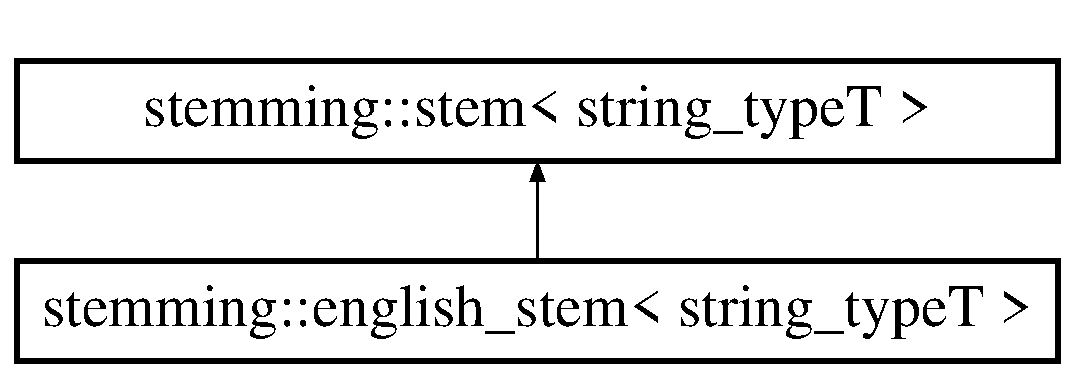
\includegraphics[height=2.000000cm]{classstemming_1_1stem}
\end{center}
\end{figure}
\subsection*{Protected Member Functions}
\begin{DoxyCompactItemize}
\item 
\hypertarget{classstemming_1_1stem_a364b7a76f683d5244715638069a4fa93}{void {\bfseries find\+\_\+r1} (const string\+\_\+type\+T \&text, const wchar\+\_\+t $\ast$vowel\+\_\+list)}\label{classstemming_1_1stem_a364b7a76f683d5244715638069a4fa93}

\item 
\hypertarget{classstemming_1_1stem_ab381c0d6a6291c2c21515e9398e83085}{void {\bfseries find\+\_\+r2} (const string\+\_\+type\+T \&text, const wchar\+\_\+t $\ast$vowel\+\_\+list)}\label{classstemming_1_1stem_ab381c0d6a6291c2c21515e9398e83085}

\item 
\hypertarget{classstemming_1_1stem_ae6cb258098ba91462d421977b1eed8e7}{void {\bfseries find\+\_\+spanish\+\_\+rv} (const string\+\_\+type\+T \&text, const wchar\+\_\+t $\ast$vowel\+\_\+list)}\label{classstemming_1_1stem_ae6cb258098ba91462d421977b1eed8e7}

\item 
\hypertarget{classstemming_1_1stem_a9626e49b982eda0d8ec3bb861d864b42}{void {\bfseries find\+\_\+french\+\_\+rv} (const string\+\_\+type\+T \&text, const wchar\+\_\+t $\ast$vowel\+\_\+list)}\label{classstemming_1_1stem_a9626e49b982eda0d8ec3bb861d864b42}

\item 
\hypertarget{classstemming_1_1stem_a53dcfe6b18fe5b5882474f222190ef1b}{void {\bfseries find\+\_\+russian\+\_\+rv} (const string\+\_\+type\+T \&text, const wchar\+\_\+t $\ast$vowel\+\_\+list)}\label{classstemming_1_1stem_a53dcfe6b18fe5b5882474f222190ef1b}

\item 
\hypertarget{classstemming_1_1stem_a9dcc3d89844ecd5c81eabf80936a0209}{void {\bfseries update\+\_\+r\+\_\+sections} (const string\+\_\+type\+T \&text)}\label{classstemming_1_1stem_a9dcc3d89844ecd5c81eabf80936a0209}

\item 
\hypertarget{classstemming_1_1stem_a34b5a8d8368dba5501b128d0710ea5c1}{void {\bfseries trim\+\_\+western\+\_\+punctuation} (string\+\_\+type\+T \&text)}\label{classstemming_1_1stem_a34b5a8d8368dba5501b128d0710ea5c1}

\item 
\hypertarget{classstemming_1_1stem_ac318ddd46a716673edf3678c47d3035c}{bool \hyperlink{classstemming_1_1stem_ac318ddd46a716673edf3678c47d3035c}{is\+\_\+suffix} (const string\+\_\+type\+T \&text, const wchar\+\_\+t suffix1\+L, const wchar\+\_\+t suffix1\+U) const }\label{classstemming_1_1stem_ac318ddd46a716673edf3678c47d3035c}

\begin{DoxyCompactList}\small\item\em is\+\_\+suffix for one character \end{DoxyCompactList}\item 
\hypertarget{classstemming_1_1stem_aad4dff424a3ae8a82dcfe6adac7c9d30}{bool \hyperlink{classstemming_1_1stem_aad4dff424a3ae8a82dcfe6adac7c9d30}{is\+\_\+suffix} (const string\+\_\+type\+T \&text, const wchar\+\_\+t suffix1\+L, const wchar\+\_\+t suffix1\+U, const wchar\+\_\+t suffix2\+L, const wchar\+\_\+t suffix2\+U) const }\label{classstemming_1_1stem_aad4dff424a3ae8a82dcfe6adac7c9d30}

\begin{DoxyCompactList}\small\item\em is\+\_\+suffix for two characters \end{DoxyCompactList}\item 
\hypertarget{classstemming_1_1stem_abbe6496d43b49dab0745e6d6b4e2831d}{bool \hyperlink{classstemming_1_1stem_abbe6496d43b49dab0745e6d6b4e2831d}{is\+\_\+suffix} (const string\+\_\+type\+T \&text, const wchar\+\_\+t suffix1\+L, const wchar\+\_\+t suffix1\+U, const wchar\+\_\+t suffix2\+L, const wchar\+\_\+t suffix2\+U, const wchar\+\_\+t suffix3\+L, const wchar\+\_\+t suffix3\+U) const }\label{classstemming_1_1stem_abbe6496d43b49dab0745e6d6b4e2831d}

\begin{DoxyCompactList}\small\item\em is\+\_\+suffix for three characters \end{DoxyCompactList}\item 
\hypertarget{classstemming_1_1stem_a694dd20e52adc89edadf120bf92a28ff}{bool \hyperlink{classstemming_1_1stem_a694dd20e52adc89edadf120bf92a28ff}{is\+\_\+suffix} (const string\+\_\+type\+T \&text, const wchar\+\_\+t suffix1\+L, const wchar\+\_\+t suffix1\+U, const wchar\+\_\+t suffix2\+L, const wchar\+\_\+t suffix2\+U, const wchar\+\_\+t suffix3\+L, const wchar\+\_\+t suffix3\+U, const wchar\+\_\+t suffix4\+L, const wchar\+\_\+t suffix4\+U) const }\label{classstemming_1_1stem_a694dd20e52adc89edadf120bf92a28ff}

\begin{DoxyCompactList}\small\item\em is\+\_\+suffix for four characters \end{DoxyCompactList}\item 
\hypertarget{classstemming_1_1stem_a001757aa7530b8acea05df8405def025}{bool \hyperlink{classstemming_1_1stem_a001757aa7530b8acea05df8405def025}{is\+\_\+suffix} (const string\+\_\+type\+T \&text, const wchar\+\_\+t suffix1\+L, const wchar\+\_\+t suffix1\+U, const wchar\+\_\+t suffix2\+L, const wchar\+\_\+t suffix2\+U, const wchar\+\_\+t suffix3\+L, const wchar\+\_\+t suffix3\+U, const wchar\+\_\+t suffix4\+L, const wchar\+\_\+t suffix4\+U, const wchar\+\_\+t suffix5\+L, const wchar\+\_\+t suffix5\+U) const }\label{classstemming_1_1stem_a001757aa7530b8acea05df8405def025}

\begin{DoxyCompactList}\small\item\em is\+\_\+suffix for five characters \end{DoxyCompactList}\item 
\hypertarget{classstemming_1_1stem_abe83f7592028b43f5cec9ce35ae1d9df}{bool \hyperlink{classstemming_1_1stem_abe83f7592028b43f5cec9ce35ae1d9df}{is\+\_\+suffix} (const string\+\_\+type\+T \&text, const wchar\+\_\+t suffix1\+L, const wchar\+\_\+t suffix1\+U, const wchar\+\_\+t suffix2\+L, const wchar\+\_\+t suffix2\+U, const wchar\+\_\+t suffix3\+L, const wchar\+\_\+t suffix3\+U, const wchar\+\_\+t suffix4\+L, const wchar\+\_\+t suffix4\+U, const wchar\+\_\+t suffix5\+L, const wchar\+\_\+t suffix5\+U, const wchar\+\_\+t suffix6\+L, const wchar\+\_\+t suffix6\+U) const }\label{classstemming_1_1stem_abe83f7592028b43f5cec9ce35ae1d9df}

\begin{DoxyCompactList}\small\item\em is\+\_\+suffix for six characters \end{DoxyCompactList}\item 
\hypertarget{classstemming_1_1stem_a79f18e256337d37054c80de470660a65}{bool \hyperlink{classstemming_1_1stem_a79f18e256337d37054c80de470660a65}{is\+\_\+suffix} (const string\+\_\+type\+T \&text, const wchar\+\_\+t suffix1\+L, const wchar\+\_\+t suffix1\+U, const wchar\+\_\+t suffix2\+L, const wchar\+\_\+t suffix2\+U, const wchar\+\_\+t suffix3\+L, const wchar\+\_\+t suffix3\+U, const wchar\+\_\+t suffix4\+L, const wchar\+\_\+t suffix4\+U, const wchar\+\_\+t suffix5\+L, const wchar\+\_\+t suffix5\+U, const wchar\+\_\+t suffix6\+L, const wchar\+\_\+t suffix6\+U, const wchar\+\_\+t suffix7\+L, const wchar\+\_\+t suffix7\+U) const }\label{classstemming_1_1stem_a79f18e256337d37054c80de470660a65}

\begin{DoxyCompactList}\small\item\em is\+\_\+suffix for seven characters \end{DoxyCompactList}\item 
\hypertarget{classstemming_1_1stem_aa18daf5b33d220d93dff22d6e591edd6}{bool \hyperlink{classstemming_1_1stem_aa18daf5b33d220d93dff22d6e591edd6}{is\+\_\+suffix} (const string\+\_\+type\+T \&text, const wchar\+\_\+t suffix1\+L, const wchar\+\_\+t suffix1\+U, const wchar\+\_\+t suffix2\+L, const wchar\+\_\+t suffix2\+U, const wchar\+\_\+t suffix3\+L, const wchar\+\_\+t suffix3\+U, const wchar\+\_\+t suffix4\+L, const wchar\+\_\+t suffix4\+U, const wchar\+\_\+t suffix5\+L, const wchar\+\_\+t suffix5\+U, const wchar\+\_\+t suffix6\+L, const wchar\+\_\+t suffix6\+U, const wchar\+\_\+t suffix7\+L, const wchar\+\_\+t suffix7\+U, const wchar\+\_\+t suffix8\+L, const wchar\+\_\+t suffix8\+U) const }\label{classstemming_1_1stem_aa18daf5b33d220d93dff22d6e591edd6}

\begin{DoxyCompactList}\small\item\em is\+\_\+suffix for eight characters \end{DoxyCompactList}\item 
\hypertarget{classstemming_1_1stem_ab905150e381f068c6b04eba851bb6263}{bool \hyperlink{classstemming_1_1stem_ab905150e381f068c6b04eba851bb6263}{is\+\_\+suffix} (const string\+\_\+type\+T \&text, const wchar\+\_\+t suffix1\+L, const wchar\+\_\+t suffix1\+U, const wchar\+\_\+t suffix2\+L, const wchar\+\_\+t suffix2\+U, const wchar\+\_\+t suffix3\+L, const wchar\+\_\+t suffix3\+U, const wchar\+\_\+t suffix4\+L, const wchar\+\_\+t suffix4\+U, const wchar\+\_\+t suffix5\+L, const wchar\+\_\+t suffix5\+U, const wchar\+\_\+t suffix6\+L, const wchar\+\_\+t suffix6\+U, const wchar\+\_\+t suffix7\+L, const wchar\+\_\+t suffix7\+U, const wchar\+\_\+t suffix8\+L, const wchar\+\_\+t suffix8\+U, const wchar\+\_\+t suffix9\+L, const wchar\+\_\+t suffix9\+U) const }\label{classstemming_1_1stem_ab905150e381f068c6b04eba851bb6263}

\begin{DoxyCompactList}\small\item\em is\+\_\+suffix for nine characterss \end{DoxyCompactList}\item 
\hypertarget{classstemming_1_1stem_a2ae63cf92bc4f4f40f0093e4842a235f}{bool \hyperlink{classstemming_1_1stem_a2ae63cf92bc4f4f40f0093e4842a235f}{is\+\_\+partial\+\_\+suffix} (const string\+\_\+type\+T \&text, const size\+\_\+t start\+\_\+index, const wchar\+\_\+t suffix1\+L, const wchar\+\_\+t suffix1\+U, const wchar\+\_\+t suffix2\+L, const wchar\+\_\+t suffix2\+U)}\label{classstemming_1_1stem_a2ae63cf92bc4f4f40f0093e4842a235f}

\begin{DoxyCompactList}\small\item\em comparison for two characters \end{DoxyCompactList}\item 
\hypertarget{classstemming_1_1stem_a728ea4e26737b04d04e02bea863f29e4}{bool \hyperlink{classstemming_1_1stem_a728ea4e26737b04d04e02bea863f29e4}{is\+\_\+partial\+\_\+suffix} (const string\+\_\+type\+T \&text, const size\+\_\+t start\+\_\+index, const wchar\+\_\+t suffix1\+L, const wchar\+\_\+t suffix1\+U, const wchar\+\_\+t suffix2\+L, const wchar\+\_\+t suffix2\+U, const wchar\+\_\+t suffix3\+L, const wchar\+\_\+t suffix3\+U)}\label{classstemming_1_1stem_a728ea4e26737b04d04e02bea863f29e4}

\begin{DoxyCompactList}\small\item\em comparison for three characters \end{DoxyCompactList}\item 
bool \hyperlink{classstemming_1_1stem_a2c92d7447b5cc97d0fca165d2b0e7d68}{is\+\_\+suffix\+\_\+in\+\_\+rv} (const string\+\_\+type\+T \&text, const wchar\+\_\+t suffix1\+L, const wchar\+\_\+t suffix1\+U)
\begin{DoxyCompactList}\small\item\em R\+V suffix functions. \end{DoxyCompactList}\item 
\hypertarget{classstemming_1_1stem_a359356fbaafc3c7154d94fda6916ffa0}{bool \hyperlink{classstemming_1_1stem_a359356fbaafc3c7154d94fda6916ffa0}{is\+\_\+suffix\+\_\+in\+\_\+rv} (const string\+\_\+type\+T \&text, const wchar\+\_\+t suffix1\+L, const wchar\+\_\+t suffix1\+U, const wchar\+\_\+t suffix2\+L, const wchar\+\_\+t suffix2\+U)}\label{classstemming_1_1stem_a359356fbaafc3c7154d94fda6916ffa0}

\begin{DoxyCompactList}\small\item\em R\+V suffix comparison for two characters. \end{DoxyCompactList}\item 
\hypertarget{classstemming_1_1stem_a00fa5d00ff53320a437fe96a5bfa8f44}{bool \hyperlink{classstemming_1_1stem_a00fa5d00ff53320a437fe96a5bfa8f44}{is\+\_\+suffix\+\_\+in\+\_\+rv} (const string\+\_\+type\+T \&text, const wchar\+\_\+t suffix1\+L, const wchar\+\_\+t suffix1\+U, const wchar\+\_\+t suffix2\+L, const wchar\+\_\+t suffix2\+U, const wchar\+\_\+t suffix3\+L, const wchar\+\_\+t suffix3\+U)}\label{classstemming_1_1stem_a00fa5d00ff53320a437fe96a5bfa8f44}

\begin{DoxyCompactList}\small\item\em R\+V suffix comparison for three characters. \end{DoxyCompactList}\item 
\hypertarget{classstemming_1_1stem_acdaff4e73f7f3841beed04775b5d4f21}{bool \hyperlink{classstemming_1_1stem_acdaff4e73f7f3841beed04775b5d4f21}{is\+\_\+suffix\+\_\+in\+\_\+rv} (const string\+\_\+type\+T \&text, const wchar\+\_\+t suffix1\+L, const wchar\+\_\+t suffix1\+U, const wchar\+\_\+t suffix2\+L, const wchar\+\_\+t suffix2\+U, const wchar\+\_\+t suffix3\+L, const wchar\+\_\+t suffix3\+U, const wchar\+\_\+t suffix4\+L, const wchar\+\_\+t suffix4\+U)}\label{classstemming_1_1stem_acdaff4e73f7f3841beed04775b5d4f21}

\begin{DoxyCompactList}\small\item\em R\+V suffix comparison for four characters. \end{DoxyCompactList}\item 
\hypertarget{classstemming_1_1stem_a99ef9b0e80da18c39cc0206a666bd4b1}{bool \hyperlink{classstemming_1_1stem_a99ef9b0e80da18c39cc0206a666bd4b1}{is\+\_\+suffix\+\_\+in\+\_\+rv} (const string\+\_\+type\+T \&text, const wchar\+\_\+t suffix1\+L, const wchar\+\_\+t suffix1\+U, const wchar\+\_\+t suffix2\+L, const wchar\+\_\+t suffix2\+U, const wchar\+\_\+t suffix3\+L, const wchar\+\_\+t suffix3\+U, const wchar\+\_\+t suffix4\+L, const wchar\+\_\+t suffix4\+U, const wchar\+\_\+t suffix5\+L, const wchar\+\_\+t suffix5\+U)}\label{classstemming_1_1stem_a99ef9b0e80da18c39cc0206a666bd4b1}

\begin{DoxyCompactList}\small\item\em R\+V suffix comparison for five characters. \end{DoxyCompactList}\item 
\hypertarget{classstemming_1_1stem_a527b081fee02f191713a50dbc396f986}{bool \hyperlink{classstemming_1_1stem_a527b081fee02f191713a50dbc396f986}{is\+\_\+suffix\+\_\+in\+\_\+rv} (const string\+\_\+type\+T \&text, const wchar\+\_\+t suffix1\+L, const wchar\+\_\+t suffix1\+U, const wchar\+\_\+t suffix2\+L, const wchar\+\_\+t suffix2\+U, const wchar\+\_\+t suffix3\+L, const wchar\+\_\+t suffix3\+U, const wchar\+\_\+t suffix4\+L, const wchar\+\_\+t suffix4\+U, const wchar\+\_\+t suffix5\+L, const wchar\+\_\+t suffix5\+U, const wchar\+\_\+t suffix6\+L, const wchar\+\_\+t suffix6\+U)}\label{classstemming_1_1stem_a527b081fee02f191713a50dbc396f986}

\begin{DoxyCompactList}\small\item\em R\+V suffix comparison for six characters. \end{DoxyCompactList}\item 
\hypertarget{classstemming_1_1stem_abd6431b54fc5175c29809c627c44a587}{bool \hyperlink{classstemming_1_1stem_abd6431b54fc5175c29809c627c44a587}{is\+\_\+suffix\+\_\+in\+\_\+rv} (const string\+\_\+type\+T \&text, const wchar\+\_\+t suffix1\+L, const wchar\+\_\+t suffix1\+U, const wchar\+\_\+t suffix2\+L, const wchar\+\_\+t suffix2\+U, const wchar\+\_\+t suffix3\+L, const wchar\+\_\+t suffix3\+U, const wchar\+\_\+t suffix4\+L, const wchar\+\_\+t suffix4\+U, const wchar\+\_\+t suffix5\+L, const wchar\+\_\+t suffix5\+U, const wchar\+\_\+t suffix6\+L, const wchar\+\_\+t suffix6\+U, const wchar\+\_\+t suffix7\+L, const wchar\+\_\+t suffix7\+U)}\label{classstemming_1_1stem_abd6431b54fc5175c29809c627c44a587}

\begin{DoxyCompactList}\small\item\em R\+V suffix comparison for seven characters. \end{DoxyCompactList}\item 
\hypertarget{classstemming_1_1stem_a553b6ed34e6b03e2c1ca42ea2db08ba6}{bool \hyperlink{classstemming_1_1stem_a553b6ed34e6b03e2c1ca42ea2db08ba6}{is\+\_\+suffix\+\_\+in\+\_\+rv} (const string\+\_\+type\+T \&text, const wchar\+\_\+t suffix1\+L, const wchar\+\_\+t suffix1\+U, const wchar\+\_\+t suffix2\+L, const wchar\+\_\+t suffix2\+U, const wchar\+\_\+t suffix3\+L, const wchar\+\_\+t suffix3\+U, const wchar\+\_\+t suffix4\+L, const wchar\+\_\+t suffix4\+U, const wchar\+\_\+t suffix5\+L, const wchar\+\_\+t suffix5\+U, const wchar\+\_\+t suffix6\+L, const wchar\+\_\+t suffix6\+U, const wchar\+\_\+t suffix7\+L, const wchar\+\_\+t suffix7\+U, const wchar\+\_\+t suffix8\+L, const wchar\+\_\+t suffix8\+U)}\label{classstemming_1_1stem_a553b6ed34e6b03e2c1ca42ea2db08ba6}

\begin{DoxyCompactList}\small\item\em R\+V suffix comparison for eight characters. \end{DoxyCompactList}\item 
bool \hyperlink{classstemming_1_1stem_aefe544e653b27bd5c1fab7b5a18d80a1}{is\+\_\+suffix\+\_\+in\+\_\+r1} (const string\+\_\+type\+T \&text, const wchar\+\_\+t suffix1\+L, const wchar\+\_\+t suffix1\+U)
\begin{DoxyCompactList}\small\item\em R1 suffix functions. \end{DoxyCompactList}\item 
\hypertarget{classstemming_1_1stem_ab8cb2e00b39091f74b1064e1f0314c6f}{bool \hyperlink{classstemming_1_1stem_ab8cb2e00b39091f74b1064e1f0314c6f}{is\+\_\+suffix\+\_\+in\+\_\+r1} (const string\+\_\+type\+T \&text, const wchar\+\_\+t suffix1\+L, const wchar\+\_\+t suffix1\+U, const wchar\+\_\+t suffix2\+L, const wchar\+\_\+t suffix2\+U)}\label{classstemming_1_1stem_ab8cb2e00b39091f74b1064e1f0314c6f}

\begin{DoxyCompactList}\small\item\em R1 suffix comparison for two characters. \end{DoxyCompactList}\item 
\hypertarget{classstemming_1_1stem_a1fe4a63adfa5d4f378a060352d52edc1}{bool \hyperlink{classstemming_1_1stem_a1fe4a63adfa5d4f378a060352d52edc1}{is\+\_\+suffix\+\_\+in\+\_\+r1} (const string\+\_\+type\+T \&text, const wchar\+\_\+t suffix1\+L, const wchar\+\_\+t suffix1\+U, const wchar\+\_\+t suffix2\+L, const wchar\+\_\+t suffix2\+U, const wchar\+\_\+t suffix3\+L, const wchar\+\_\+t suffix3\+U)}\label{classstemming_1_1stem_a1fe4a63adfa5d4f378a060352d52edc1}

\begin{DoxyCompactList}\small\item\em R1 suffix comparison for three characters. \end{DoxyCompactList}\item 
\hypertarget{classstemming_1_1stem_a3fef2f8916933fa1965928f8e43a1b58}{bool \hyperlink{classstemming_1_1stem_a3fef2f8916933fa1965928f8e43a1b58}{is\+\_\+suffix\+\_\+in\+\_\+r1} (const string\+\_\+type\+T \&text, const wchar\+\_\+t suffix1\+L, const wchar\+\_\+t suffix1\+U, const wchar\+\_\+t suffix2\+L, const wchar\+\_\+t suffix2\+U, const wchar\+\_\+t suffix3\+L, const wchar\+\_\+t suffix3\+U, const wchar\+\_\+t suffix4\+L, const wchar\+\_\+t suffix4\+U)}\label{classstemming_1_1stem_a3fef2f8916933fa1965928f8e43a1b58}

\begin{DoxyCompactList}\small\item\em R1 suffix comparison for four characters. \end{DoxyCompactList}\item 
\hypertarget{classstemming_1_1stem_a88f0e5e0cc055f013b6321215eb18ef3}{bool \hyperlink{classstemming_1_1stem_a88f0e5e0cc055f013b6321215eb18ef3}{is\+\_\+suffix\+\_\+in\+\_\+r1} (const string\+\_\+type\+T \&text, const wchar\+\_\+t suffix1\+L, const wchar\+\_\+t suffix1\+U, const wchar\+\_\+t suffix2\+L, const wchar\+\_\+t suffix2\+U, const wchar\+\_\+t suffix3\+L, const wchar\+\_\+t suffix3\+U, const wchar\+\_\+t suffix4\+L, const wchar\+\_\+t suffix4\+U, const wchar\+\_\+t suffix5\+L, const wchar\+\_\+t suffix5\+U)}\label{classstemming_1_1stem_a88f0e5e0cc055f013b6321215eb18ef3}

\begin{DoxyCompactList}\small\item\em R1 suffix comparison for five characters. \end{DoxyCompactList}\item 
\hypertarget{classstemming_1_1stem_a19c2ee5166c7a9c81160408438c1f9a0}{bool \hyperlink{classstemming_1_1stem_a19c2ee5166c7a9c81160408438c1f9a0}{is\+\_\+suffix\+\_\+in\+\_\+r1} (const string\+\_\+type\+T \&text, const wchar\+\_\+t suffix1\+L, const wchar\+\_\+t suffix1\+U, const wchar\+\_\+t suffix2\+L, const wchar\+\_\+t suffix2\+U, const wchar\+\_\+t suffix3\+L, const wchar\+\_\+t suffix3\+U, const wchar\+\_\+t suffix4\+L, const wchar\+\_\+t suffix4\+U, const wchar\+\_\+t suffix5\+L, const wchar\+\_\+t suffix5\+U, const wchar\+\_\+t suffix6\+L, const wchar\+\_\+t suffix6\+U)}\label{classstemming_1_1stem_a19c2ee5166c7a9c81160408438c1f9a0}

\begin{DoxyCompactList}\small\item\em R1 suffix comparison for six characters. \end{DoxyCompactList}\item 
bool \hyperlink{classstemming_1_1stem_ac2c9cace7e6d90ca0b8c08f2ca2809e3}{is\+\_\+suffix\+\_\+in\+\_\+r2} (const string\+\_\+type\+T \&text, const wchar\+\_\+t suffix1\+L, const wchar\+\_\+t suffix1\+U)
\begin{DoxyCompactList}\small\item\em R2 suffix functions. \end{DoxyCompactList}\item 
\hypertarget{classstemming_1_1stem_a8325bde2b5c8d5676d2b8e2b822b29a4}{bool \hyperlink{classstemming_1_1stem_a8325bde2b5c8d5676d2b8e2b822b29a4}{is\+\_\+suffix\+\_\+in\+\_\+r2} (const string\+\_\+type\+T \&text, const wchar\+\_\+t suffix1\+L, const wchar\+\_\+t suffix1\+U, const wchar\+\_\+t suffix2\+L, const wchar\+\_\+t suffix2\+U)}\label{classstemming_1_1stem_a8325bde2b5c8d5676d2b8e2b822b29a4}

\begin{DoxyCompactList}\small\item\em R2 suffix comparison for two characters. \end{DoxyCompactList}\item 
\hypertarget{classstemming_1_1stem_ab5c71d01e3285eec2e79521c1b76f79d}{bool \hyperlink{classstemming_1_1stem_ab5c71d01e3285eec2e79521c1b76f79d}{is\+\_\+suffix\+\_\+in\+\_\+r2} (const string\+\_\+type\+T \&text, const wchar\+\_\+t suffix1\+L, const wchar\+\_\+t suffix1\+U, const wchar\+\_\+t suffix2\+L, const wchar\+\_\+t suffix2\+U, const wchar\+\_\+t suffix3\+L, const wchar\+\_\+t suffix3\+U)}\label{classstemming_1_1stem_ab5c71d01e3285eec2e79521c1b76f79d}

\begin{DoxyCompactList}\small\item\em R2 suffix comparison for three characters. \end{DoxyCompactList}\item 
\hypertarget{classstemming_1_1stem_ac12e9f11d41f69e71c7379387c4564b9}{bool \hyperlink{classstemming_1_1stem_ac12e9f11d41f69e71c7379387c4564b9}{is\+\_\+suffix\+\_\+in\+\_\+r2} (const string\+\_\+type\+T \&text, const wchar\+\_\+t suffix1\+L, const wchar\+\_\+t suffix1\+U, const wchar\+\_\+t suffix2\+L, const wchar\+\_\+t suffix2\+U, const wchar\+\_\+t suffix3\+L, const wchar\+\_\+t suffix3\+U, const wchar\+\_\+t suffix4\+L, const wchar\+\_\+t suffix4\+U)}\label{classstemming_1_1stem_ac12e9f11d41f69e71c7379387c4564b9}

\begin{DoxyCompactList}\small\item\em R2 suffix comparison for four characters. \end{DoxyCompactList}\item 
\hypertarget{classstemming_1_1stem_aca8fba0d6b27d8da969508adc281cfa5}{bool \hyperlink{classstemming_1_1stem_aca8fba0d6b27d8da969508adc281cfa5}{is\+\_\+suffix\+\_\+in\+\_\+r2} (const string\+\_\+type\+T \&text, const wchar\+\_\+t suffix1\+L, const wchar\+\_\+t suffix1\+U, const wchar\+\_\+t suffix2\+L, const wchar\+\_\+t suffix2\+U, const wchar\+\_\+t suffix3\+L, const wchar\+\_\+t suffix3\+U, const wchar\+\_\+t suffix4\+L, const wchar\+\_\+t suffix4\+U, const wchar\+\_\+t suffix5\+L, const wchar\+\_\+t suffix5\+U)}\label{classstemming_1_1stem_aca8fba0d6b27d8da969508adc281cfa5}

\begin{DoxyCompactList}\small\item\em R2 suffix comparison for five characters. \end{DoxyCompactList}\item 
\hypertarget{classstemming_1_1stem_ad85a9757083c5fcbd6300367df2a648b}{bool \hyperlink{classstemming_1_1stem_ad85a9757083c5fcbd6300367df2a648b}{is\+\_\+suffix\+\_\+in\+\_\+r2} (string\+\_\+type\+T \&text, const wchar\+\_\+t suffix1\+L, const wchar\+\_\+t suffix1\+U, const wchar\+\_\+t suffix2\+L, const wchar\+\_\+t suffix2\+U, const wchar\+\_\+t suffix3\+L, const wchar\+\_\+t suffix3\+U, const wchar\+\_\+t suffix4\+L, const wchar\+\_\+t suffix4\+U, const wchar\+\_\+t suffix5\+L, const wchar\+\_\+t suffix5\+U, const wchar\+\_\+t suffix6\+L, const wchar\+\_\+t suffix6\+U)}\label{classstemming_1_1stem_ad85a9757083c5fcbd6300367df2a648b}

\begin{DoxyCompactList}\small\item\em R2 suffix comparison for six characters. \end{DoxyCompactList}\item 
\hypertarget{classstemming_1_1stem_a65e9882d17885e66208840b277fcee2e}{bool \hyperlink{classstemming_1_1stem_a65e9882d17885e66208840b277fcee2e}{is\+\_\+suffix\+\_\+in\+\_\+r2} (const string\+\_\+type\+T \&text, const wchar\+\_\+t suffix1\+L, const wchar\+\_\+t suffix1\+U, const wchar\+\_\+t suffix2\+L, const wchar\+\_\+t suffix2\+U, const wchar\+\_\+t suffix3\+L, const wchar\+\_\+t suffix3\+U, const wchar\+\_\+t suffix4\+L, const wchar\+\_\+t suffix4\+U, const wchar\+\_\+t suffix5\+L, const wchar\+\_\+t suffix5\+U, const wchar\+\_\+t suffix6\+L, const wchar\+\_\+t suffix6\+U, const wchar\+\_\+t suffix7\+L, const wchar\+\_\+t suffix7\+U)}\label{classstemming_1_1stem_a65e9882d17885e66208840b277fcee2e}

\begin{DoxyCompactList}\small\item\em R2 suffix comparison for seven characters. \end{DoxyCompactList}\item 
\hypertarget{classstemming_1_1stem_a3bda630783eae1661f00fc5d2b51ce5c}{bool {\bfseries delete\+\_\+if\+\_\+is\+\_\+in\+\_\+r1} (string\+\_\+type\+T \&text, const wchar\+\_\+t suffix1\+L, const wchar\+\_\+t suffix1\+U, const bool success\+\_\+on\+\_\+find=true)}\label{classstemming_1_1stem_a3bda630783eae1661f00fc5d2b51ce5c}

\item 
\hypertarget{classstemming_1_1stem_a843e54b874cbb56a5d5997987137c933}{bool {\bfseries delete\+\_\+if\+\_\+is\+\_\+in\+\_\+r1} (string\+\_\+type\+T \&text, const wchar\+\_\+t suffix1\+L, const wchar\+\_\+t suffix1\+U, const wchar\+\_\+t suffix2\+L, const wchar\+\_\+t suffix2\+U, const bool success\+\_\+on\+\_\+find=true)}\label{classstemming_1_1stem_a843e54b874cbb56a5d5997987137c933}

\item 
\hypertarget{classstemming_1_1stem_af5c33c5c4644373cd85390c7e3282084}{bool {\bfseries delete\+\_\+if\+\_\+is\+\_\+in\+\_\+r1} (string\+\_\+type\+T \&text, const wchar\+\_\+t suffix1\+L, const wchar\+\_\+t suffix1\+U, const wchar\+\_\+t suffix2\+L, const wchar\+\_\+t suffix2\+U, const wchar\+\_\+t suffix3\+L, const wchar\+\_\+t suffix3\+U, const bool success\+\_\+on\+\_\+find=true)}\label{classstemming_1_1stem_af5c33c5c4644373cd85390c7e3282084}

\item 
\hypertarget{classstemming_1_1stem_a6be1595a7c29fec666ff808701be3eb2}{bool {\bfseries delete\+\_\+if\+\_\+is\+\_\+in\+\_\+r1} (string\+\_\+type\+T \&text, const wchar\+\_\+t suffix1\+L, const wchar\+\_\+t suffix1\+U, const wchar\+\_\+t suffix2\+L, const wchar\+\_\+t suffix2\+U, const wchar\+\_\+t suffix3\+L, const wchar\+\_\+t suffix3\+U, const wchar\+\_\+t suffix4\+L, const wchar\+\_\+t suffix4\+U, const bool success\+\_\+on\+\_\+find=true)}\label{classstemming_1_1stem_a6be1595a7c29fec666ff808701be3eb2}

\item 
\hypertarget{classstemming_1_1stem_abac9ef13a80efee3dad9b72476f7cd49}{bool {\bfseries delete\+\_\+if\+\_\+is\+\_\+in\+\_\+r1} (string\+\_\+type\+T \&text, const wchar\+\_\+t suffix1\+L, const wchar\+\_\+t suffix1\+U, const wchar\+\_\+t suffix2\+L, const wchar\+\_\+t suffix2\+U, const wchar\+\_\+t suffix3\+L, const wchar\+\_\+t suffix3\+U, const wchar\+\_\+t suffix4\+L, const wchar\+\_\+t suffix4\+U, const wchar\+\_\+t suffix5\+L, const wchar\+\_\+t suffix5\+U, const bool success\+\_\+on\+\_\+find=true)}\label{classstemming_1_1stem_abac9ef13a80efee3dad9b72476f7cd49}

\item 
\hypertarget{classstemming_1_1stem_a3fbbd1cbf322889ba4e4940d87449bb0}{bool {\bfseries delete\+\_\+if\+\_\+is\+\_\+in\+\_\+r1} (string\+\_\+type\+T \&text, const wchar\+\_\+t suffix1\+L, const wchar\+\_\+t suffix1\+U, const wchar\+\_\+t suffix2\+L, const wchar\+\_\+t suffix2\+U, const wchar\+\_\+t suffix3\+L, const wchar\+\_\+t suffix3\+U, const wchar\+\_\+t suffix4\+L, const wchar\+\_\+t suffix4\+U, const wchar\+\_\+t suffix5\+L, const wchar\+\_\+t suffix5\+U, const wchar\+\_\+t suffix6\+L, const wchar\+\_\+t suffix6\+U, const bool success\+\_\+on\+\_\+find=true)}\label{classstemming_1_1stem_a3fbbd1cbf322889ba4e4940d87449bb0}

\item 
\hypertarget{classstemming_1_1stem_acdf0457bd3392f1ac23dadef5515cebd}{bool {\bfseries delete\+\_\+if\+\_\+is\+\_\+in\+\_\+r1} (string\+\_\+type\+T \&text, const wchar\+\_\+t suffix1\+L, const wchar\+\_\+t suffix1\+U, const wchar\+\_\+t suffix2\+L, const wchar\+\_\+t suffix2\+U, const wchar\+\_\+t suffix3\+L, const wchar\+\_\+t suffix3\+U, const wchar\+\_\+t suffix4\+L, const wchar\+\_\+t suffix4\+U, const wchar\+\_\+t suffix5\+L, const wchar\+\_\+t suffix5\+U, const wchar\+\_\+t suffix6\+L, const wchar\+\_\+t suffix6\+U, const wchar\+\_\+t suffix7\+L, const wchar\+\_\+t suffix7\+U, const bool success\+\_\+on\+\_\+find=true)}\label{classstemming_1_1stem_acdf0457bd3392f1ac23dadef5515cebd}

\item 
\hypertarget{classstemming_1_1stem_a722e75e6404934da2f0c9c00ffded48a}{bool {\bfseries delete\+\_\+if\+\_\+is\+\_\+in\+\_\+r2} (string\+\_\+type\+T \&text, const wchar\+\_\+t suffix1\+L, const wchar\+\_\+t suffix1\+U, const bool success\+\_\+on\+\_\+find=true)}\label{classstemming_1_1stem_a722e75e6404934da2f0c9c00ffded48a}

\item 
\hypertarget{classstemming_1_1stem_a33bf1854d1748ba97e30ad798f828b0e}{bool {\bfseries delete\+\_\+if\+\_\+is\+\_\+in\+\_\+r2} (string\+\_\+type\+T \&text, const wchar\+\_\+t suffix1\+L, const wchar\+\_\+t suffix1\+U, const wchar\+\_\+t suffix2\+L, const wchar\+\_\+t suffix2\+U, const bool success\+\_\+on\+\_\+find=true)}\label{classstemming_1_1stem_a33bf1854d1748ba97e30ad798f828b0e}

\item 
\hypertarget{classstemming_1_1stem_ac78dd58f01ed17a41eedc33d5b2deedb}{bool {\bfseries delete\+\_\+if\+\_\+is\+\_\+in\+\_\+r2} (string\+\_\+type\+T \&text, const wchar\+\_\+t suffix1\+L, const wchar\+\_\+t suffix1\+U, const wchar\+\_\+t suffix2\+L, const wchar\+\_\+t suffix2\+U, const wchar\+\_\+t suffix3\+L, const wchar\+\_\+t suffix3\+U, const bool success\+\_\+on\+\_\+find=true)}\label{classstemming_1_1stem_ac78dd58f01ed17a41eedc33d5b2deedb}

\item 
\hypertarget{classstemming_1_1stem_a3a79fd0ac96d009d0c93f1bec847c2ff}{bool {\bfseries delete\+\_\+if\+\_\+is\+\_\+in\+\_\+r2} (string\+\_\+type\+T \&text, const wchar\+\_\+t suffix1\+L, const wchar\+\_\+t suffix1\+U, const wchar\+\_\+t suffix2\+L, const wchar\+\_\+t suffix2\+U, const wchar\+\_\+t suffix3\+L, const wchar\+\_\+t suffix3\+U, const wchar\+\_\+t suffix4\+L, const wchar\+\_\+t suffix4\+U, const bool success\+\_\+on\+\_\+find=true)}\label{classstemming_1_1stem_a3a79fd0ac96d009d0c93f1bec847c2ff}

\item 
\hypertarget{classstemming_1_1stem_a222f7af1124d34e58b3c38fa4b2ee669}{bool \hyperlink{classstemming_1_1stem_a222f7af1124d34e58b3c38fa4b2ee669}{delete\+\_\+if\+\_\+is\+\_\+in\+\_\+r2} (string\+\_\+type\+T \&text, const wchar\+\_\+t suffix1\+L, const wchar\+\_\+t suffix1\+U, const wchar\+\_\+t suffix2\+L, const wchar\+\_\+t suffix2\+U, const wchar\+\_\+t suffix3\+L, const wchar\+\_\+t suffix3\+U, const wchar\+\_\+t suffix4\+L, const wchar\+\_\+t suffix4\+U, const wchar\+\_\+t suffix5\+L, const wchar\+\_\+t suffix5\+U, const bool success\+\_\+on\+\_\+find=true)}\label{classstemming_1_1stem_a222f7af1124d34e58b3c38fa4b2ee669}

\begin{DoxyCompactList}\small\item\em R2 deletion for five character suffix. \end{DoxyCompactList}\item 
\hypertarget{classstemming_1_1stem_a95aca52d1f624638130a9d1c66570edb}{bool \hyperlink{classstemming_1_1stem_a95aca52d1f624638130a9d1c66570edb}{delete\+\_\+if\+\_\+is\+\_\+in\+\_\+r2} (string\+\_\+type\+T \&text, const wchar\+\_\+t suffix1\+L, const wchar\+\_\+t suffix1\+U, const wchar\+\_\+t suffix2\+L, const wchar\+\_\+t suffix2\+U, const wchar\+\_\+t suffix3\+L, const wchar\+\_\+t suffix3\+U, const wchar\+\_\+t suffix4\+L, const wchar\+\_\+t suffix4\+U, const wchar\+\_\+t suffix5\+L, const wchar\+\_\+t suffix5\+U, const wchar\+\_\+t suffix6\+L, const wchar\+\_\+t suffix6\+U, const bool success\+\_\+on\+\_\+find=true)}\label{classstemming_1_1stem_a95aca52d1f624638130a9d1c66570edb}

\begin{DoxyCompactList}\small\item\em R2 deletion for six character suffix. \end{DoxyCompactList}\item 
\hypertarget{classstemming_1_1stem_a9542e67a264c728cfb636767dc75a07c}{bool \hyperlink{classstemming_1_1stem_a9542e67a264c728cfb636767dc75a07c}{delete\+\_\+if\+\_\+is\+\_\+in\+\_\+r2} (string\+\_\+type\+T \&text, const wchar\+\_\+t suffix1\+L, const wchar\+\_\+t suffix1\+U, const wchar\+\_\+t suffix2\+L, const wchar\+\_\+t suffix2\+U, const wchar\+\_\+t suffix3\+L, const wchar\+\_\+t suffix3\+U, const wchar\+\_\+t suffix4\+L, const wchar\+\_\+t suffix4\+U, const wchar\+\_\+t suffix5\+L, const wchar\+\_\+t suffix5\+U, const wchar\+\_\+t suffix6\+L, const wchar\+\_\+t suffix6\+U, const wchar\+\_\+t suffix7\+L, const wchar\+\_\+t suffix7\+U, const bool success\+\_\+on\+\_\+find=true)}\label{classstemming_1_1stem_a9542e67a264c728cfb636767dc75a07c}

\begin{DoxyCompactList}\small\item\em R2 deletion for seven character suffix. \end{DoxyCompactList}\item 
\hypertarget{classstemming_1_1stem_a9bbc2192839ce8ebcf88d0220cfa2441}{bool \hyperlink{classstemming_1_1stem_a9bbc2192839ce8ebcf88d0220cfa2441}{delete\+\_\+if\+\_\+is\+\_\+in\+\_\+r2} (string\+\_\+type\+T \&text, const wchar\+\_\+t suffix1\+L, const wchar\+\_\+t suffix1\+U, const wchar\+\_\+t suffix2\+L, const wchar\+\_\+t suffix2\+U, const wchar\+\_\+t suffix3\+L, const wchar\+\_\+t suffix3\+U, const wchar\+\_\+t suffix4\+L, const wchar\+\_\+t suffix4\+U, const wchar\+\_\+t suffix5\+L, const wchar\+\_\+t suffix5\+U, const wchar\+\_\+t suffix6\+L, const wchar\+\_\+t suffix6\+U, const wchar\+\_\+t suffix7\+L, const wchar\+\_\+t suffix7\+U, const wchar\+\_\+t suffix8\+L, const wchar\+\_\+t suffix8\+U, const bool success\+\_\+on\+\_\+find=true)}\label{classstemming_1_1stem_a9bbc2192839ce8ebcf88d0220cfa2441}

\begin{DoxyCompactList}\small\item\em R2 deletion for eight character suffix. \end{DoxyCompactList}\item 
\hypertarget{classstemming_1_1stem_a3754d998db70ac20861ab3e87c3e5f25}{bool {\bfseries delete\+\_\+if\+\_\+is\+\_\+in\+\_\+rv} (string\+\_\+type\+T \&text, const wchar\+\_\+t suffix1\+L, const wchar\+\_\+t suffix1\+U, const bool success\+\_\+on\+\_\+find=true)}\label{classstemming_1_1stem_a3754d998db70ac20861ab3e87c3e5f25}

\item 
\hypertarget{classstemming_1_1stem_a5d0a95806d9264f7238bf425311d1dfc}{bool {\bfseries delete\+\_\+if\+\_\+is\+\_\+in\+\_\+rv} (string\+\_\+type\+T \&text, const wchar\+\_\+t suffix1\+L, const wchar\+\_\+t suffix1\+U, const wchar\+\_\+t suffix2\+L, const wchar\+\_\+t suffix2\+U, const bool success\+\_\+on\+\_\+find=true)}\label{classstemming_1_1stem_a5d0a95806d9264f7238bf425311d1dfc}

\item 
\hypertarget{classstemming_1_1stem_a70623a86bd9b759befe998a364d2bad2}{bool {\bfseries delete\+\_\+if\+\_\+is\+\_\+in\+\_\+rv} (string\+\_\+type\+T \&text, const wchar\+\_\+t suffix1\+L, const wchar\+\_\+t suffix1\+U, const wchar\+\_\+t suffix2\+L, const wchar\+\_\+t suffix2\+U, const wchar\+\_\+t suffix3\+L, const wchar\+\_\+t suffix3\+U, const bool success\+\_\+on\+\_\+find=true)}\label{classstemming_1_1stem_a70623a86bd9b759befe998a364d2bad2}

\item 
\hypertarget{classstemming_1_1stem_aa14e355385422f170a184e1e2182c6b0}{bool {\bfseries delete\+\_\+if\+\_\+is\+\_\+in\+\_\+rv} (string\+\_\+type\+T \&text, const wchar\+\_\+t suffix1\+L, const wchar\+\_\+t suffix1\+U, const wchar\+\_\+t suffix2\+L, const wchar\+\_\+t suffix2\+U, const wchar\+\_\+t suffix3\+L, const wchar\+\_\+t suffix3\+U, const wchar\+\_\+t suffix4\+L, const wchar\+\_\+t suffix4\+U, const bool success\+\_\+on\+\_\+find=true)}\label{classstemming_1_1stem_aa14e355385422f170a184e1e2182c6b0}

\item 
\hypertarget{classstemming_1_1stem_adb10d6f58dca24420ce2b1fd7e58928f}{bool {\bfseries delete\+\_\+if\+\_\+is\+\_\+in\+\_\+rv} (string\+\_\+type\+T \&text, const wchar\+\_\+t suffix1\+L, const wchar\+\_\+t suffix1\+U, const wchar\+\_\+t suffix2\+L, const wchar\+\_\+t suffix2\+U, const wchar\+\_\+t suffix3\+L, const wchar\+\_\+t suffix3\+U, const wchar\+\_\+t suffix4\+L, const wchar\+\_\+t suffix4\+U, const wchar\+\_\+t suffix5\+L, const wchar\+\_\+t suffix5\+U, const bool success\+\_\+on\+\_\+find=true)}\label{classstemming_1_1stem_adb10d6f58dca24420ce2b1fd7e58928f}

\item 
\hypertarget{classstemming_1_1stem_a2102feb734da90e80172d1f34102c8cd}{bool {\bfseries delete\+\_\+if\+\_\+is\+\_\+in\+\_\+rv} (string\+\_\+type\+T \&text, const wchar\+\_\+t suffix1\+L, const wchar\+\_\+t suffix1\+U, const wchar\+\_\+t suffix2\+L, const wchar\+\_\+t suffix2\+U, const wchar\+\_\+t suffix3\+L, const wchar\+\_\+t suffix3\+U, const wchar\+\_\+t suffix4\+L, const wchar\+\_\+t suffix4\+U, const wchar\+\_\+t suffix5\+L, const wchar\+\_\+t suffix5\+U, const wchar\+\_\+t suffix6\+L, const wchar\+\_\+t suffix6\+U, const bool success\+\_\+on\+\_\+find=true)}\label{classstemming_1_1stem_a2102feb734da90e80172d1f34102c8cd}

\item 
\hypertarget{classstemming_1_1stem_acc427221d55bf93e113f2811eedca74a}{bool {\bfseries delete\+\_\+if\+\_\+is\+\_\+in\+\_\+rv} (string\+\_\+type\+T \&text, const wchar\+\_\+t suffix1\+L, const wchar\+\_\+t suffix1\+U, const wchar\+\_\+t suffix2\+L, const wchar\+\_\+t suffix2\+U, const wchar\+\_\+t suffix3\+L, const wchar\+\_\+t suffix3\+U, const wchar\+\_\+t suffix4\+L, const wchar\+\_\+t suffix4\+U, const wchar\+\_\+t suffix5\+L, const wchar\+\_\+t suffix5\+U, const wchar\+\_\+t suffix6\+L, const wchar\+\_\+t suffix6\+U, const wchar\+\_\+t suffix7\+L, const wchar\+\_\+t suffix7\+U, const bool success\+\_\+on\+\_\+find=true)}\label{classstemming_1_1stem_acc427221d55bf93e113f2811eedca74a}

\item 
\hypertarget{classstemming_1_1stem_ab0b50197480905de68f3be29714860d7}{bool {\bfseries delete\+\_\+if\+\_\+is\+\_\+in\+\_\+rv} (string\+\_\+type\+T \&text, const wchar\+\_\+t suffix1\+L, const wchar\+\_\+t suffix1\+U, const wchar\+\_\+t suffix2\+L, const wchar\+\_\+t suffix2\+U, const wchar\+\_\+t suffix3\+L, const wchar\+\_\+t suffix3\+U, const wchar\+\_\+t suffix4\+L, const wchar\+\_\+t suffix4\+U, const wchar\+\_\+t suffix5\+L, const wchar\+\_\+t suffix5\+U, const wchar\+\_\+t suffix6\+L, const wchar\+\_\+t suffix6\+U, const wchar\+\_\+t suffix7\+L, const wchar\+\_\+t suffix7\+U, const wchar\+\_\+t suffix8\+L, const wchar\+\_\+t suffix8\+U, const bool success\+\_\+on\+\_\+find=true)}\label{classstemming_1_1stem_ab0b50197480905de68f3be29714860d7}

\item 
\hypertarget{classstemming_1_1stem_a760765796790f28c1acfa3b1e603781d}{void {\bfseries remove\+\_\+german\+\_\+umlauts} (string\+\_\+type\+T \&text)}\label{classstemming_1_1stem_a760765796790f28c1acfa3b1e603781d}

\item 
\hypertarget{classstemming_1_1stem_a85e349feabc837fa38ceb40cbfe8f16e}{void {\bfseries italian\+\_\+acutes\+\_\+to\+\_\+graves} (string\+\_\+type\+T \&text)}\label{classstemming_1_1stem_a85e349feabc837fa38ceb40cbfe8f16e}

\item 
\hypertarget{classstemming_1_1stem_ad7324f61a80140d122da1c087289b737}{void \hyperlink{classstemming_1_1stem_ad7324f61a80140d122da1c087289b737}{hash\+\_\+dutch\+\_\+yi} (string\+\_\+type\+T \&text, const wchar\+\_\+t $\ast$vowel\+\_\+string)}\label{classstemming_1_1stem_ad7324f61a80140d122da1c087289b737}

\begin{DoxyCompactList}\small\item\em Hash initial y, y after a vowel, and i between vowels into hashed character. \end{DoxyCompactList}\item 
\hypertarget{classstemming_1_1stem_a00a03f9e29573b89ff269e3832aa019b}{void {\bfseries unhash\+\_\+dutch\+\_\+yi} (string\+\_\+type\+T \&text)}\label{classstemming_1_1stem_a00a03f9e29573b89ff269e3832aa019b}

\item 
\hypertarget{classstemming_1_1stem_a2ab335f89cb2e65564a7985156d6ce19}{void \hyperlink{classstemming_1_1stem_a2ab335f89cb2e65564a7985156d6ce19}{hash\+\_\+german\+\_\+yu} (string\+\_\+type\+T \&text, const wchar\+\_\+t $\ast$vowel\+\_\+string)}\label{classstemming_1_1stem_a2ab335f89cb2e65564a7985156d6ce19}

\begin{DoxyCompactList}\small\item\em Hash 'u' and 'y' between vowels. \end{DoxyCompactList}\item 
\hypertarget{classstemming_1_1stem_a70ee7015775ebb7d8b98a1724f94448e}{void {\bfseries unhash\+\_\+german\+\_\+yu} (string\+\_\+type\+T \&text)}\label{classstemming_1_1stem_a70ee7015775ebb7d8b98a1724f94448e}

\item 
void \hyperlink{classstemming_1_1stem_a0fa77155cef02f4efa2a537450ef4004}{hash\+\_\+french\+\_\+yui} (string\+\_\+type\+T \&text, const wchar\+\_\+t $\ast$vowel\+\_\+string)
\item 
\hypertarget{classstemming_1_1stem_a11e5585424ce623ee7842a039bdfb7cb}{void {\bfseries unhash\+\_\+french\+\_\+yui} (string\+\_\+type\+T \&text)}\label{classstemming_1_1stem_a11e5585424ce623ee7842a039bdfb7cb}

\item 
\hypertarget{classstemming_1_1stem_ab7cc895f7a16b9bec4a4c4614111ecb3}{void {\bfseries hash\+\_\+y} (string\+\_\+type\+T \&text, const wchar\+\_\+t $\ast$vowel\+\_\+string)}\label{classstemming_1_1stem_ab7cc895f7a16b9bec4a4c4614111ecb3}

\item 
\hypertarget{classstemming_1_1stem_acc93df08d3d68d2468aa3e7cf23c7089}{void {\bfseries unhash\+\_\+y} (string\+\_\+type\+T \&text)}\label{classstemming_1_1stem_acc93df08d3d68d2468aa3e7cf23c7089}

\item 
\hypertarget{classstemming_1_1stem_a11d05105fc3e03bd5f2ff581bc4eb6fe}{void \hyperlink{classstemming_1_1stem_a11d05105fc3e03bd5f2ff581bc4eb6fe}{hash\+\_\+italian\+\_\+ui} (string\+\_\+type\+T \&text, const wchar\+\_\+t $\ast$vowel\+\_\+string)}\label{classstemming_1_1stem_a11d05105fc3e03bd5f2ff581bc4eb6fe}

\begin{DoxyCompactList}\small\item\em Hash u after q, and u, i between vowels. \end{DoxyCompactList}\item 
\hypertarget{classstemming_1_1stem_ab4f2f7360665b96d941ba614dc3d5092}{void {\bfseries unhash\+\_\+italian\+\_\+ui} (string\+\_\+type\+T \&text)}\label{classstemming_1_1stem_ab4f2f7360665b96d941ba614dc3d5092}

\item 
\hypertarget{classstemming_1_1stem_a44d995c39f2a31089ae3505fb483cbfa}{void {\bfseries remove\+\_\+dutch\+\_\+umlauts} (string\+\_\+type\+T \&text)}\label{classstemming_1_1stem_a44d995c39f2a31089ae3505fb483cbfa}

\item 
\hypertarget{classstemming_1_1stem_a42ba7697636adbf2d757c360a981920f}{void {\bfseries remove\+\_\+dutch\+\_\+acutes} (string\+\_\+type\+T \&text)}\label{classstemming_1_1stem_a42ba7697636adbf2d757c360a981920f}

\item 
\hypertarget{classstemming_1_1stem_a0b3535733088736897f35f8d925c92e9}{void {\bfseries remove\+\_\+spanish\+\_\+acutes} (string\+\_\+type\+T \&text)}\label{classstemming_1_1stem_a0b3535733088736897f35f8d925c92e9}

\item 
\hypertarget{classstemming_1_1stem_a09ab497dfe31fc007c70d7f7d790fa51}{size\+\_\+t {\bfseries get\+\_\+r1} () const }\label{classstemming_1_1stem_a09ab497dfe31fc007c70d7f7d790fa51}

\item 
\hypertarget{classstemming_1_1stem_a87fa173343063b5e85722edefe493ab5}{void {\bfseries set\+\_\+r1} (const size\+\_\+t val)}\label{classstemming_1_1stem_a87fa173343063b5e85722edefe493ab5}

\item 
\hypertarget{classstemming_1_1stem_a90aba2c99e1fa12883eba32211089f3b}{size\+\_\+t {\bfseries get\+\_\+r2} () const }\label{classstemming_1_1stem_a90aba2c99e1fa12883eba32211089f3b}

\item 
\hypertarget{classstemming_1_1stem_a032bb774988c5b8f6fae7cf28b59d485}{void {\bfseries set\+\_\+r2} (const size\+\_\+t val)}\label{classstemming_1_1stem_a032bb774988c5b8f6fae7cf28b59d485}

\item 
\hypertarget{classstemming_1_1stem_aefa75f006e0b4b623a2608dc23dff605}{size\+\_\+t {\bfseries get\+\_\+rv} () const }\label{classstemming_1_1stem_aefa75f006e0b4b623a2608dc23dff605}

\item 
\hypertarget{classstemming_1_1stem_a1fda692e873dfcae7048679ffdb29a5e}{void {\bfseries set\+\_\+rv} (const size\+\_\+t val)}\label{classstemming_1_1stem_a1fda692e873dfcae7048679ffdb29a5e}

\item 
\hypertarget{classstemming_1_1stem_acefba08458c6a8cc00a733afb3a064ed}{void {\bfseries reset\+\_\+r\+\_\+values} ()}\label{classstemming_1_1stem_acefba08458c6a8cc00a733afb3a064ed}

\end{DoxyCompactItemize}


\subsection{Member Function Documentation}
\hypertarget{classstemming_1_1stem_a0fa77155cef02f4efa2a537450ef4004}{\index{stemming\+::stem@{stemming\+::stem}!hash\+\_\+french\+\_\+yui@{hash\+\_\+french\+\_\+yui}}
\index{hash\+\_\+french\+\_\+yui@{hash\+\_\+french\+\_\+yui}!stemming\+::stem@{stemming\+::stem}}
\subsubsection[{hash\+\_\+french\+\_\+yui}]{\setlength{\rightskip}{0pt plus 5cm}template$<$typename string\+\_\+type\+T  = std\+::wstring$>$ void {\bf stemming\+::stem}$<$ string\+\_\+type\+T $>$\+::hash\+\_\+french\+\_\+yui (
\begin{DoxyParamCaption}
\item[{string\+\_\+type\+T \&}]{text, }
\item[{const wchar\+\_\+t $\ast$}]{vowel\+\_\+string}
\end{DoxyParamCaption}
)\hspace{0.3cm}{\ttfamily [inline]}, {\ttfamily [protected]}}}\label{classstemming_1_1stem_a0fa77155cef02f4efa2a537450ef4004}
Hash u or i preceded and followed by a vowel, and y preceded or followed by a vowel. u after q is also hashed. For example, jouer -\/$>$ jo\+Uer ennuie -\/$>$ ennu\+Ie yeux -\/$>$ Yeux quand -\/$>$ q\+Uand \hypertarget{classstemming_1_1stem_aefe544e653b27bd5c1fab7b5a18d80a1}{\index{stemming\+::stem@{stemming\+::stem}!is\+\_\+suffix\+\_\+in\+\_\+r1@{is\+\_\+suffix\+\_\+in\+\_\+r1}}
\index{is\+\_\+suffix\+\_\+in\+\_\+r1@{is\+\_\+suffix\+\_\+in\+\_\+r1}!stemming\+::stem@{stemming\+::stem}}
\subsubsection[{is\+\_\+suffix\+\_\+in\+\_\+r1}]{\setlength{\rightskip}{0pt plus 5cm}template$<$typename string\+\_\+type\+T  = std\+::wstring$>$ bool {\bf stemming\+::stem}$<$ string\+\_\+type\+T $>$\+::is\+\_\+suffix\+\_\+in\+\_\+r1 (
\begin{DoxyParamCaption}
\item[{const string\+\_\+type\+T \&}]{text, }
\item[{const wchar\+\_\+t}]{suffix1\+L, }
\item[{const wchar\+\_\+t}]{suffix1\+U}
\end{DoxyParamCaption}
)\hspace{0.3cm}{\ttfamily [inline]}, {\ttfamily [protected]}}}\label{classstemming_1_1stem_aefe544e653b27bd5c1fab7b5a18d80a1}


R1 suffix functions. 

R1 suffix comparison for one character \hypertarget{classstemming_1_1stem_ac2c9cace7e6d90ca0b8c08f2ca2809e3}{\index{stemming\+::stem@{stemming\+::stem}!is\+\_\+suffix\+\_\+in\+\_\+r2@{is\+\_\+suffix\+\_\+in\+\_\+r2}}
\index{is\+\_\+suffix\+\_\+in\+\_\+r2@{is\+\_\+suffix\+\_\+in\+\_\+r2}!stemming\+::stem@{stemming\+::stem}}
\subsubsection[{is\+\_\+suffix\+\_\+in\+\_\+r2}]{\setlength{\rightskip}{0pt plus 5cm}template$<$typename string\+\_\+type\+T  = std\+::wstring$>$ bool {\bf stemming\+::stem}$<$ string\+\_\+type\+T $>$\+::is\+\_\+suffix\+\_\+in\+\_\+r2 (
\begin{DoxyParamCaption}
\item[{const string\+\_\+type\+T \&}]{text, }
\item[{const wchar\+\_\+t}]{suffix1\+L, }
\item[{const wchar\+\_\+t}]{suffix1\+U}
\end{DoxyParamCaption}
)\hspace{0.3cm}{\ttfamily [inline]}, {\ttfamily [protected]}}}\label{classstemming_1_1stem_ac2c9cace7e6d90ca0b8c08f2ca2809e3}


R2 suffix functions. 

R2 suffix comparison for one character \hypertarget{classstemming_1_1stem_a2c92d7447b5cc97d0fca165d2b0e7d68}{\index{stemming\+::stem@{stemming\+::stem}!is\+\_\+suffix\+\_\+in\+\_\+rv@{is\+\_\+suffix\+\_\+in\+\_\+rv}}
\index{is\+\_\+suffix\+\_\+in\+\_\+rv@{is\+\_\+suffix\+\_\+in\+\_\+rv}!stemming\+::stem@{stemming\+::stem}}
\subsubsection[{is\+\_\+suffix\+\_\+in\+\_\+rv}]{\setlength{\rightskip}{0pt plus 5cm}template$<$typename string\+\_\+type\+T  = std\+::wstring$>$ bool {\bf stemming\+::stem}$<$ string\+\_\+type\+T $>$\+::is\+\_\+suffix\+\_\+in\+\_\+rv (
\begin{DoxyParamCaption}
\item[{const string\+\_\+type\+T \&}]{text, }
\item[{const wchar\+\_\+t}]{suffix1\+L, }
\item[{const wchar\+\_\+t}]{suffix1\+U}
\end{DoxyParamCaption}
)\hspace{0.3cm}{\ttfamily [inline]}, {\ttfamily [protected]}}}\label{classstemming_1_1stem_a2c92d7447b5cc97d0fca165d2b0e7d68}


R\+V suffix functions. 

R\+V suffix comparison for one character 

The documentation for this class was generated from the following file\+:\begin{DoxyCompactItemize}
\item 
stemming.\+h\end{DoxyCompactItemize}

\hypertarget{class_stem_helper}{}\section{Stem\+Helper Class Reference}
\label{class_stem_helper}\index{Stem\+Helper@{Stem\+Helper}}


{\ttfamily \#include $<$stem\+Helper.\+h$>$}

\subsection*{Static Public Member Functions}
\begin{DoxyCompactItemize}
\item 
static std\+::string \hyperlink{class_stem_helper_af2878d595387afb436bb38ae0a1c9f4d}{stemword} (char $\ast$buffer)
\end{DoxyCompactItemize}


\subsection{Member Function Documentation}
\hypertarget{class_stem_helper_af2878d595387afb436bb38ae0a1c9f4d}{}\index{Stem\+Helper@{Stem\+Helper}!stemword@{stemword}}
\index{stemword@{stemword}!Stem\+Helper@{Stem\+Helper}}
\subsubsection[{stemword}]{\setlength{\rightskip}{0pt plus 5cm}static std\+::string Stem\+Helper\+::stemword (
\begin{DoxyParamCaption}
\item[{char $\ast$}]{buffer}
\end{DoxyParamCaption}
)\hspace{0.3cm}{\ttfamily [inline]}, {\ttfamily [static]}}\label{class_stem_helper_af2878d595387afb436bb38ae0a1c9f4d}


The documentation for this class was generated from the following file\+:\begin{DoxyCompactItemize}
\item 
\hyperlink{stem_helper_8h}{stem\+Helper.\+h}\end{DoxyCompactItemize}

\hypertarget{structstemmer}{}\section{stemmer Struct Reference}
\label{structstemmer}\index{stemmer@{stemmer}}


{\ttfamily \#include $<$Porter\+Stemmer.\+h$>$}

\subsection*{Public Attributes}
\begin{DoxyCompactItemize}
\item 
char $\ast$ \hyperlink{structstemmer_a0ae99db94786418a0c4d85a2a15382a5}{b}
\item 
int \hyperlink{structstemmer_a587d5f8fd5c491688bc91e7d3b5e262e}{k}
\item 
int \hyperlink{structstemmer_a024d42a47e06bd5207e2494cbfefbf2f}{j}
\end{DoxyCompactItemize}


\subsection{Member Data Documentation}
\hypertarget{structstemmer_a0ae99db94786418a0c4d85a2a15382a5}{}\index{stemmer@{stemmer}!b@{b}}
\index{b@{b}!stemmer@{stemmer}}
\subsubsection[{b}]{\setlength{\rightskip}{0pt plus 5cm}char$\ast$ stemmer\+::b}\label{structstemmer_a0ae99db94786418a0c4d85a2a15382a5}
\hypertarget{structstemmer_a024d42a47e06bd5207e2494cbfefbf2f}{}\index{stemmer@{stemmer}!j@{j}}
\index{j@{j}!stemmer@{stemmer}}
\subsubsection[{j}]{\setlength{\rightskip}{0pt plus 5cm}int stemmer\+::j}\label{structstemmer_a024d42a47e06bd5207e2494cbfefbf2f}
\hypertarget{structstemmer_a587d5f8fd5c491688bc91e7d3b5e262e}{}\index{stemmer@{stemmer}!k@{k}}
\index{k@{k}!stemmer@{stemmer}}
\subsubsection[{k}]{\setlength{\rightskip}{0pt plus 5cm}int stemmer\+::k}\label{structstemmer_a587d5f8fd5c491688bc91e7d3b5e262e}


The documentation for this struct was generated from the following file\+:\begin{DoxyCompactItemize}
\item 
\hyperlink{_porter_stemmer_8h}{Porter\+Stemmer.\+h}\end{DoxyCompactItemize}

\hypertarget{classstring__util_1_1string__trim}{\section{string\+\_\+util\+:\+:string\+\_\+trim$<$ char\+\_\+type\+T $>$ Class Template Reference}
\label{classstring__util_1_1string__trim}\index{string\+\_\+util\+::string\+\_\+trim$<$ char\+\_\+type\+T $>$@{string\+\_\+util\+::string\+\_\+trim$<$ char\+\_\+type\+T $>$}}
}


trims whitespace from around a string  




{\ttfamily \#include $<$string\+\_\+util.\+h$>$}

\subsection*{Public Member Functions}
\begin{DoxyCompactItemize}
\item 
\hypertarget{classstring__util_1_1string__trim_a33ce709a5bd7a1fd2d974a0940fc1ff8}{const char\+\_\+type\+T $\ast$ {\bfseries operator()} (const char\+\_\+type\+T $\ast$value, size\+\_\+t length=std\+::basic\+\_\+string$<$ char\+\_\+type\+T $>$\+::npos)}\label{classstring__util_1_1string__trim_a33ce709a5bd7a1fd2d974a0940fc1ff8}

\item 
\hypertarget{classstring__util_1_1string__trim_abea837c5d6ef343a91b161d039162ecb}{size\+\_\+t {\bfseries get\+\_\+trimmed\+\_\+string\+\_\+length} () const }\label{classstring__util_1_1string__trim_abea837c5d6ef343a91b161d039162ecb}

\end{DoxyCompactItemize}


\subsection{Detailed Description}
\subsubsection*{template$<$typename char\+\_\+type\+T$>$class string\+\_\+util\+::string\+\_\+trim$<$ char\+\_\+type\+T $>$}

trims whitespace from around a string 

The documentation for this class was generated from the following file\+:\begin{DoxyCompactItemize}
\item 
string\+\_\+util.\+h\end{DoxyCompactItemize}

\hypertarget{class_user_interface}{\section{User\+Interface Class Reference}
\label{class_user_interface}\index{User\+Interface@{User\+Interface}}
}
\subsection*{Public Member Functions}
\begin{DoxyCompactItemize}
\item 
\hypertarget{class_user_interface_a5f668ba7e20441556650a2ab57919eb8}{void {\bfseries driver} ()}\label{class_user_interface_a5f668ba7e20441556650a2ab57919eb8}

\item 
\hypertarget{class_user_interface_aef424faaaab1a26e7e95615953dfb6b5}{void {\bfseries maintenence\+Mode} ()}\label{class_user_interface_aef424faaaab1a26e7e95615953dfb6b5}

\item 
\hypertarget{class_user_interface_a31406e8b5be6361c5e45f4f9b873c995}{void {\bfseries interactive\+Mode} ()}\label{class_user_interface_a31406e8b5be6361c5e45f4f9b873c995}

\item 
\hypertarget{class_user_interface_a0e9d6f1de4247604921f008ad8fd488b}{void {\bfseries stress\+Test} ()}\label{class_user_interface_a0e9d6f1de4247604921f008ad8fd488b}

\item 
\hypertarget{class_user_interface_a2b38e64d7c7cd64d09e8719ff747b244}{bool {\bfseries fexists} (const string \&)}\label{class_user_interface_a2b38e64d7c7cd64d09e8719ff747b244}

\item 
\hypertarget{class_user_interface_ac6235e19919c71faf514f82ae89b922f}{void {\bfseries clear\+Index} ()}\label{class_user_interface_ac6235e19919c71faf514f82ae89b922f}

\item 
\hypertarget{class_user_interface_a5aae71a73a68b9876c5ce7b1cba54910}{void {\bfseries add\+Files\+To\+Index} ()}\label{class_user_interface_a5aae71a73a68b9876c5ce7b1cba54910}

\item 
\hypertarget{class_user_interface_a6afb3103066951f4f3c69931cea544de}{void {\bfseries create\+Structure} (string)}\label{class_user_interface_a6afb3103066951f4f3c69931cea544de}

\item 
\hypertarget{class_user_interface_a141bf602a34bc9e85176bf05f3889ad2}{void {\bfseries add\+To\+Existing\+Index} ()}\label{class_user_interface_a141bf602a34bc9e85176bf05f3889ad2}

\end{DoxyCompactItemize}


The documentation for this class was generated from the following files\+:\begin{DoxyCompactItemize}
\item 
User\+Interface.\+h\item 
User\+Interface.\+cpp\end{DoxyCompactItemize}

\hypertarget{classwithin}{\section{within$<$ T $>$ Class Template Reference}
\label{classwithin}\index{within$<$ T $>$@{within$<$ T $>$}}
}
Inheritance diagram for within$<$ T $>$\+:\begin{figure}[H]
\begin{center}
\leavevmode
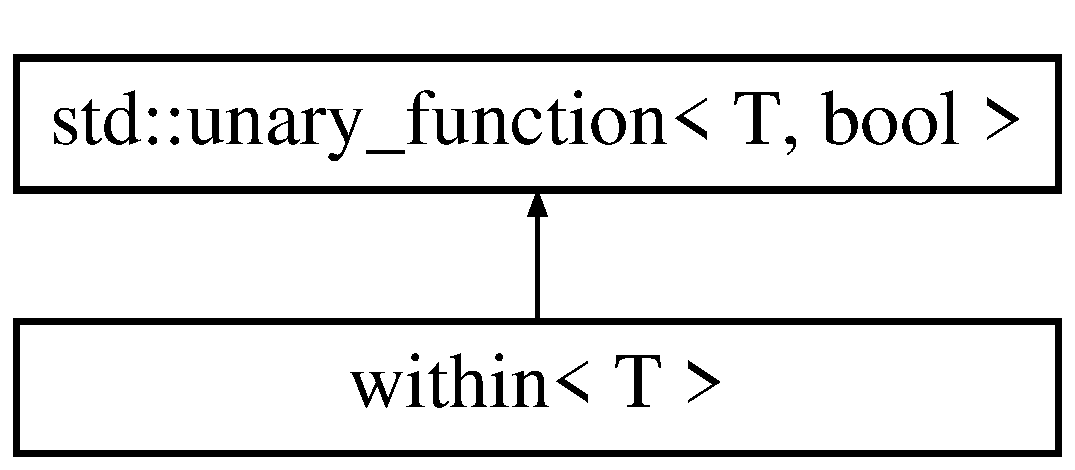
\includegraphics[height=2.000000cm]{classwithin}
\end{center}
\end{figure}
\subsection*{Public Member Functions}
\begin{DoxyCompactItemize}
\item 
\hypertarget{classwithin_ac461f80eef6cbe70a69729fd5b99f751}{{\bfseries within} (T range\+\_\+begin, T range\+\_\+end)}\label{classwithin_ac461f80eef6cbe70a69729fd5b99f751}

\item 
\hypertarget{classwithin_aaab5ecca0235613f499bc5e607d23cbd}{bool {\bfseries operator()} (T value) const }\label{classwithin_aaab5ecca0235613f499bc5e607d23cbd}

\end{DoxyCompactItemize}


The documentation for this class was generated from the following file\+:\begin{DoxyCompactItemize}
\item 
utilities.\+h\end{DoxyCompactItemize}

\chapter{Example Documentation}
\hypertarget{_2_users_2sam_2_documents_2_d_s_search_engine_project_2code_2stemming_8h-example}{\section{/\+Users/sam/\+Documents/\+D\+S\+Search\+Engine\+Project/code/stemming.\+h}
}
The template argument for the stemmers are the type of std\+::basic\+\_\+string that you are trying to stem, by default std\+::wstring (Unicode strings). As long as the char type of your basic\+\_\+string is wchar\+\_\+t, then you can use any type of basic\+\_\+string. This is to say, if your basic\+\_\+string has a custom char\+\_\+traits or allocator, then just specify it in your template argument to the stemmer.

typedef std\+::basic\+\_\+string$<$wchar\+\_\+t, my\+Traits, my\+Allocator$>$ my\+String;~\newline
 my\+String word(L\char`\"{}documentation\char`\"{});~\newline
 stemming\+::english\+\_\+stem$<$my\+String$>$ Stem\+English;~\newline
 Stem\+English(word);


\begin{DoxyCodeInclude}
\end{DoxyCodeInclude}
 
%--- End generated contents ---

% Index
\newpage
\phantomsection
\addcontentsline{toc}{chapter}{Index}
\printindex

\end{document}
